% LaTex Template

\documentclass[12pt]{article}
\usepackage{natbib}
\usepackage[letterpaper, margin=1.1in]{geometry}
\usepackage{graphicx}
\usepackage{wrapfig}
\usepackage{enumitem}
\setlist[enumerate]{itemsep=0mm}
\usepackage{multirow}
\usepackage{lscape}
\usepackage{caption}
\usepackage{subcaption}

\begin{document}
\noindent{Alexandra Pulwicki \\ \today}

\begin{center}
\Large \textbf{Field Methods and Report \\ May 2016}
\end{center}


\section*{Overview}

A winter snow survey was conducted on three glaciers in the Donjek Range of the St. Elias Mountains in May 2016. This report documents the field design and planning, how the planned work was implemented in the field, and a summary of each day. 

***Still needed: close up photo of swe tube, snowpit cut outs?

***Transects = Linear and curvilinear transects

***cite snow school for measuring with probe technique?

\tableofcontents
\pagebreak

%%%%
\section{Field Design}
%%%%

\subsection{Sampling Scheme and Naming System}

Three glaciers within the Donjek Range were chosen as study sites and can be seen in Figure \ref{studysites}. Glaciers in the Donjek Range are unnamed but working names have been employed by \cite{Crompton2016} and are adopted for this work. Glacier 4, Glacier 2, and Glacier 13 were selected. These glaciers were chosen because these glaciers are spread throughout the Donjek Range and are located increasingly further from the large-scale topographic divide (located at the head of the Kaskawalsh Glacier \citep{Taylor1969}). The three glaciers are also located on different sides of the range-scale topographic divides, which run roughly from west to east in the southern area and from south to north in the eastern area and form an `L' shape. Glacier 4 is located on the southern side of the first arm, Glacier 2 is located on the northern side of the first arm and the western side of the second arm, and Glacier 13 is located on the eastern side of the second arm. The selected glaciers also have similar orientations and one central glacier-filled valley (similar shape). Within the Donjek Range, these glaciers have good SPOT5 DEM coverage, which provides the highest resolution DEM available for this area. Additionally, the majority of the three glaciers is accessible on foot and the total area is small enough (see Table \ref{glacierstats}) to allow for reasonable coverage using point measurements.

\begin{table}[b!]
\centering
\caption{Area, length, and elevation descriptors of three chosen glaciers.}
\label{glacierstats}
\begin{tabular}{|l|c|c|ccc|}
\hline
\multicolumn{1}{|c|}{} & \multirow{2}{*}{\textbf{Area (km$^2$)}} & \multirow{2}{*}{\textbf{Length (km)}} & \multicolumn{3}{c|}{\textbf{Elevation (m)}}         \\
\multicolumn{1}{|c|}{} &                                         &                                       & \textbf{Minimum} & \textbf{Maximum} & \textbf{Mean} \\ \hline
Glacier 4              & 5.26                                    & 6.2                                   & 1573             & 2854             & 2321          \\
Glacier 2              & 6.91                                    & 7.4                                   & 1906             & 3098             & 2472          \\
Glacier 13             & 12.33                                   & 9.5                                   & 1775             & 3037             & 2434          \\ \hline
\end{tabular}
\end{table} 

The sampling scheme for each glacier was chosen to be similar so that comparison between glaciers could be done more readily. Each glacier was divided into the accumulation area, upper ablation area, and lower ablation area. In the accumulation area, a central snowpit location was chosen. Additionally, a series of approximately ten snow coring locations was chosen throughout the accumulation area. Steep sections and glacier margins were avoided. In both the upper and lower ablation area, an `hourglass and circle' (Parr, C., 2016 personal communication) as well as a transverse (below the hourglass) and midline transect were mapped out. The length and width of each shape was adjusted to span the full dimension of its corresponding area. Snowpit locations in the ablation area were chosen to be at the centre of each hourglass. An overview of the sampling design can be seen in Figure \ref{transect_planned}.

The full ablation area was also divided into seven zones of approximately equal elevation intervals. Three locations within each zone were then randomly selected for zigzag \citep{Shea2010} measurements (Figure \ref{zigzag_planned}) and the three locations were randomly labelled as different priorities. The goal was to complete one zigzag in each zone. If possible, the measurement would be completed at the `Priority A' location but if it was not possible due to dangerous conditions then the `Priority B' or `Priority C' locations would be chosen. This allowed for random locations to be used but with the flexibility to adjust locations in the field. SWE measurements would be taken within each zigzag, and at snowpit locations with the ablation area.  

The location of each snow depth and density measurement is imported into hand-held GPS devices (Garmin GPSMAP 64s) as a waypoint with a unique name. Points that are part of a transect have a name with the glacier number, the transect and area that the point belongs to, and a three-digit sequential number. The code for the transect area and type includes two letters. The first letter is either `A' for `accumulation area', `U' for `upper ablation area', or `L' for `lower ablation area'. The second letter indicates the transect type, with `H' for `hourglass', `T' for `transverse transect', `C' for `circle', and `M' for `midline'. For example, the name G04\_UM023 is the 23rd point on the Midline transect in the Upper ablation area of Glacier 4, and G13\_LC134 is the 134th point on the circle in the lower ablation area of Glacier 13. Other points that are not part of a transect also follow a similar naming convention. The snowpit locations use the code `SP' (e.g. G04\_LSP is the snowpit located in the lower ablation zone of Glacier 4) and the firn coring locations have the code `FC' and a two digit number (e.g. G02\_AFC04 is the fourth firn core location in the accumulation area of Glacier 2).

The zigzag points have a name with the glacier number, the zone that they were located in, the zigzag priority, and the vertex number. The zone and priority (A, B, C) are indicated by a `Z', then the zone number, and then an `A', `B', or `C'. The vertex number is indicated by a `ZZ' and then a sequential number. For example, the vertex labelled G02\_Z2C\_ZZ04 is on Glacier 2 in zone 2 and the fourth point of a priority C zigzag. The vertex labelled G13\_Z7A\_ZZ08 is on Glacier 13 in zone 7 and the eighth point of a priority A zigzag. An example of a zigzag sampling scheme can be seen in Figure \ref{zigzag_vertex}.

\begin{landscape}
\begin{figure}
	\centering
	\fbox{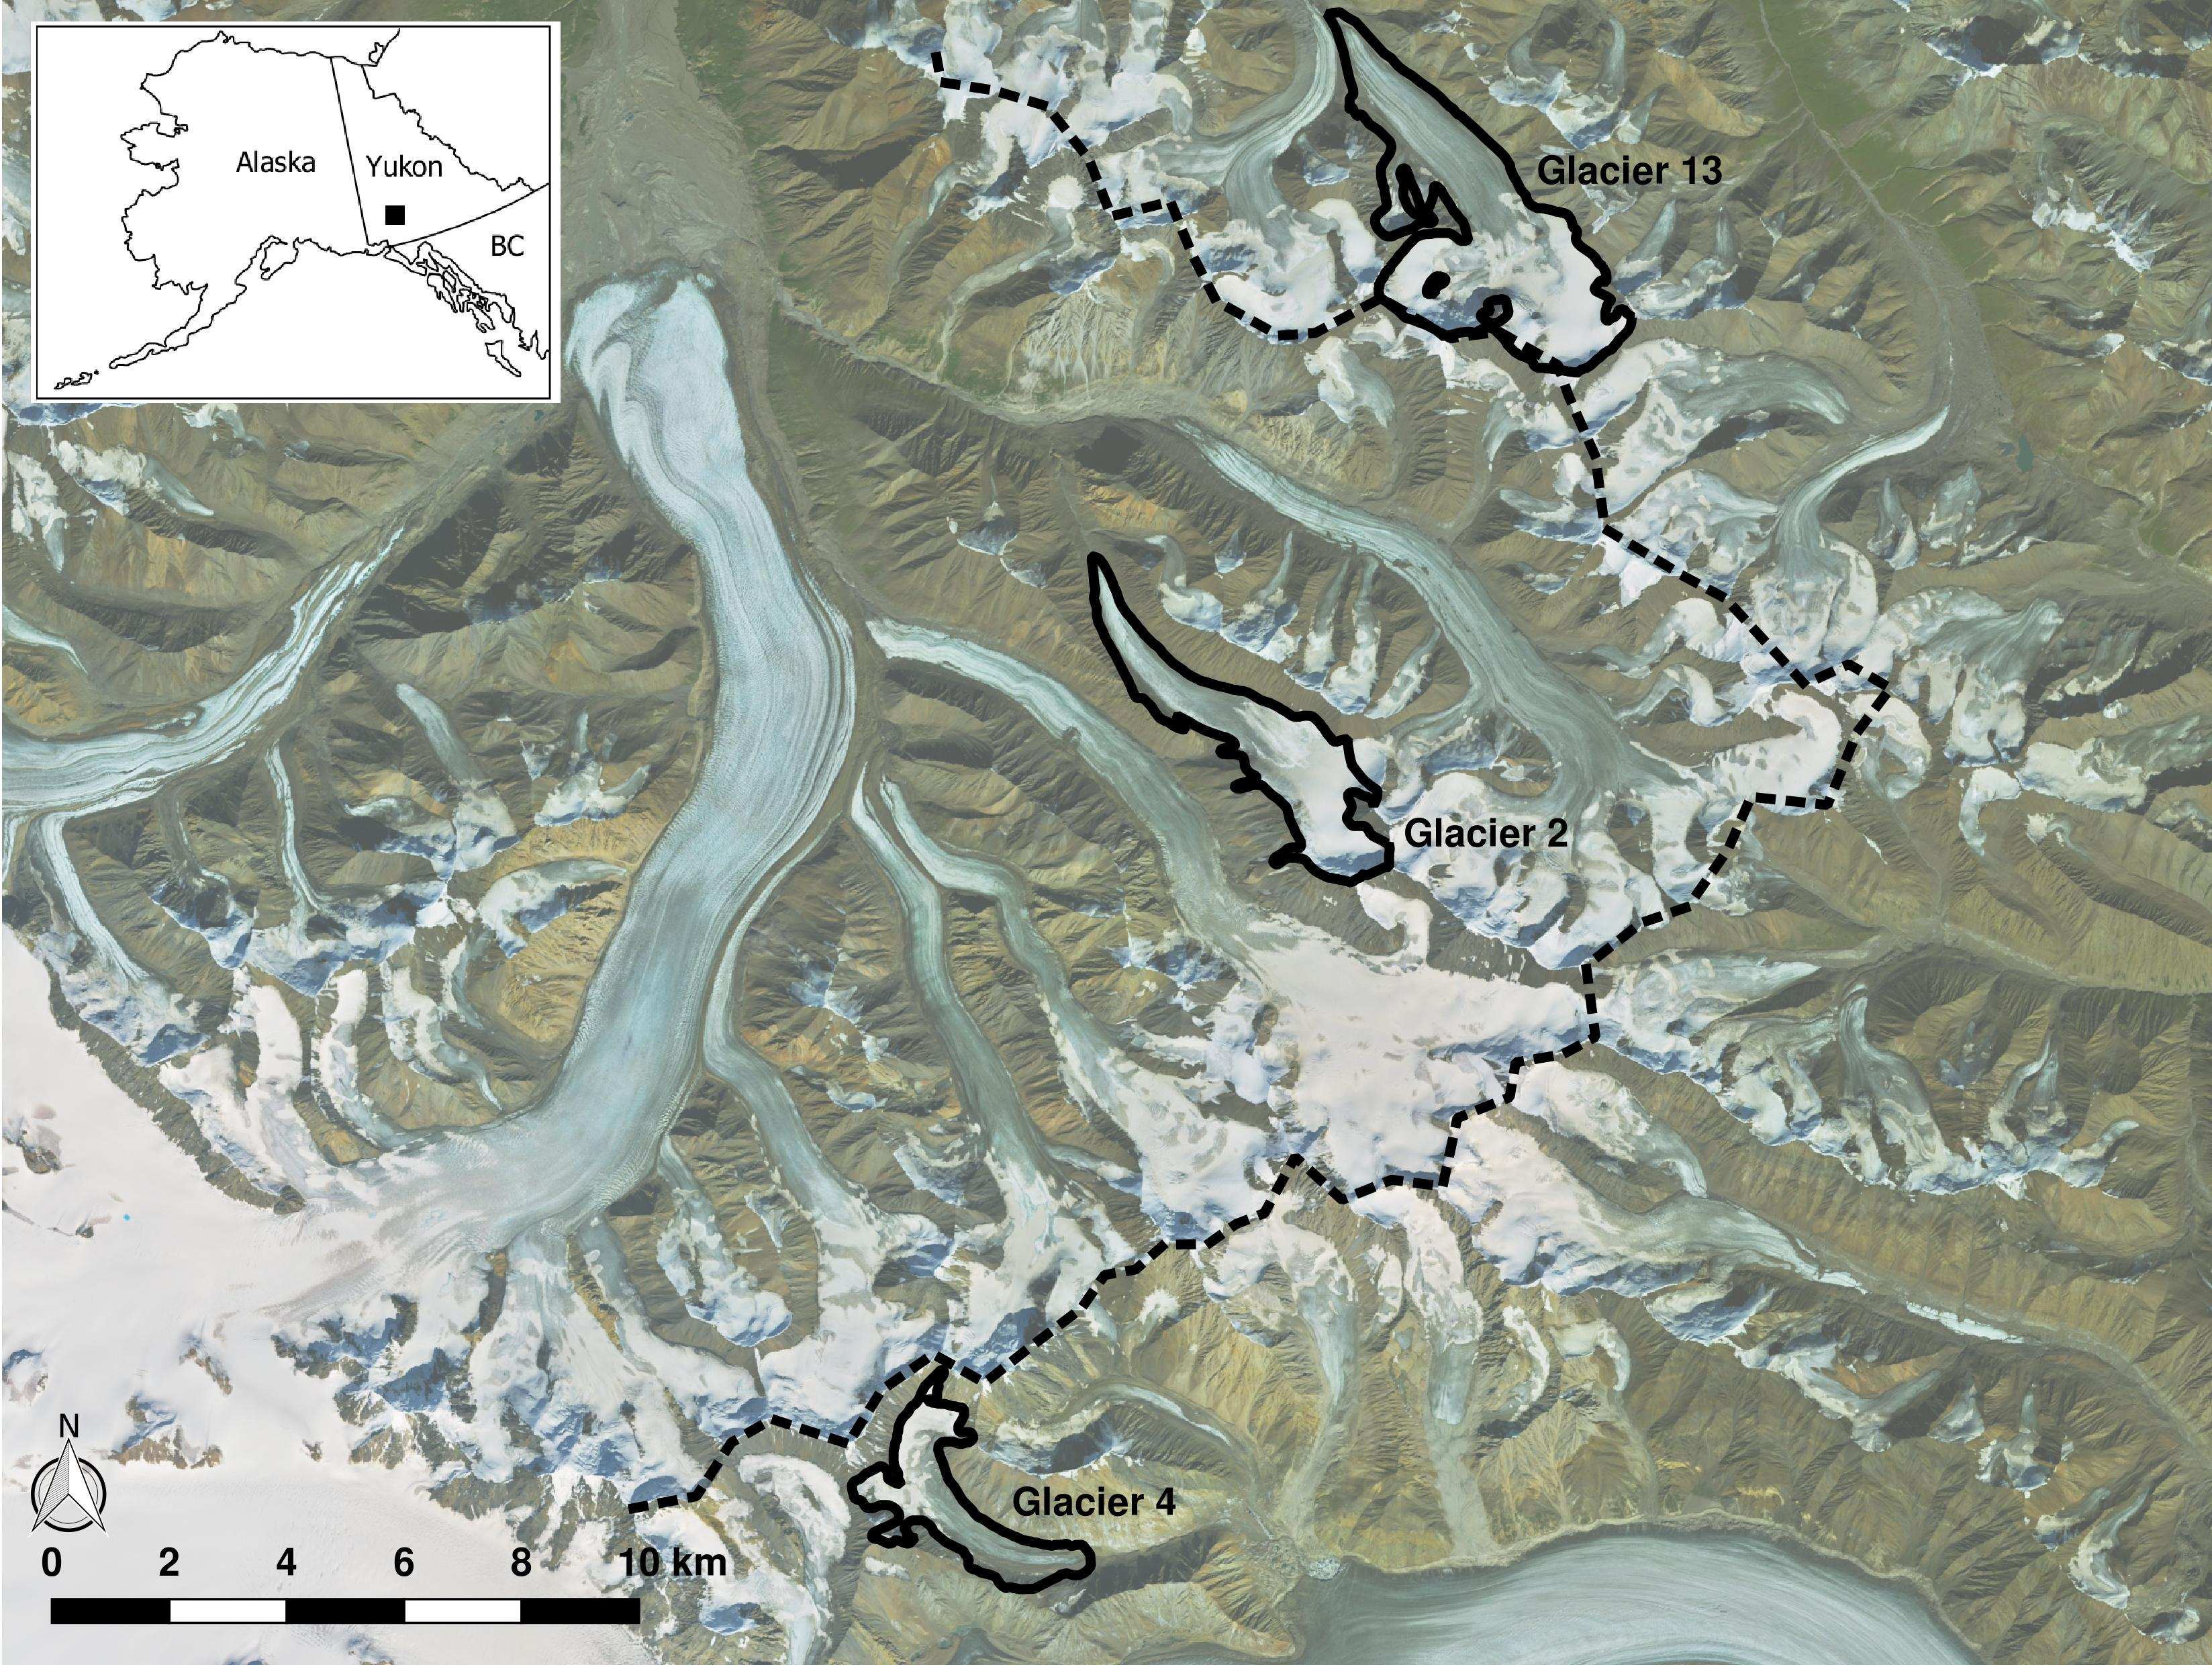
\includegraphics[height = 0.95\textwidth]{chosenglaciers.jpeg}}\\
	\caption{Study glaciers in the Donjek Range, Yukon (see inset). The topographic divide is shown as a dashed line.}
	\label{studysites}
\end{figure}

\begin{figure}
	\centering
	\fbox{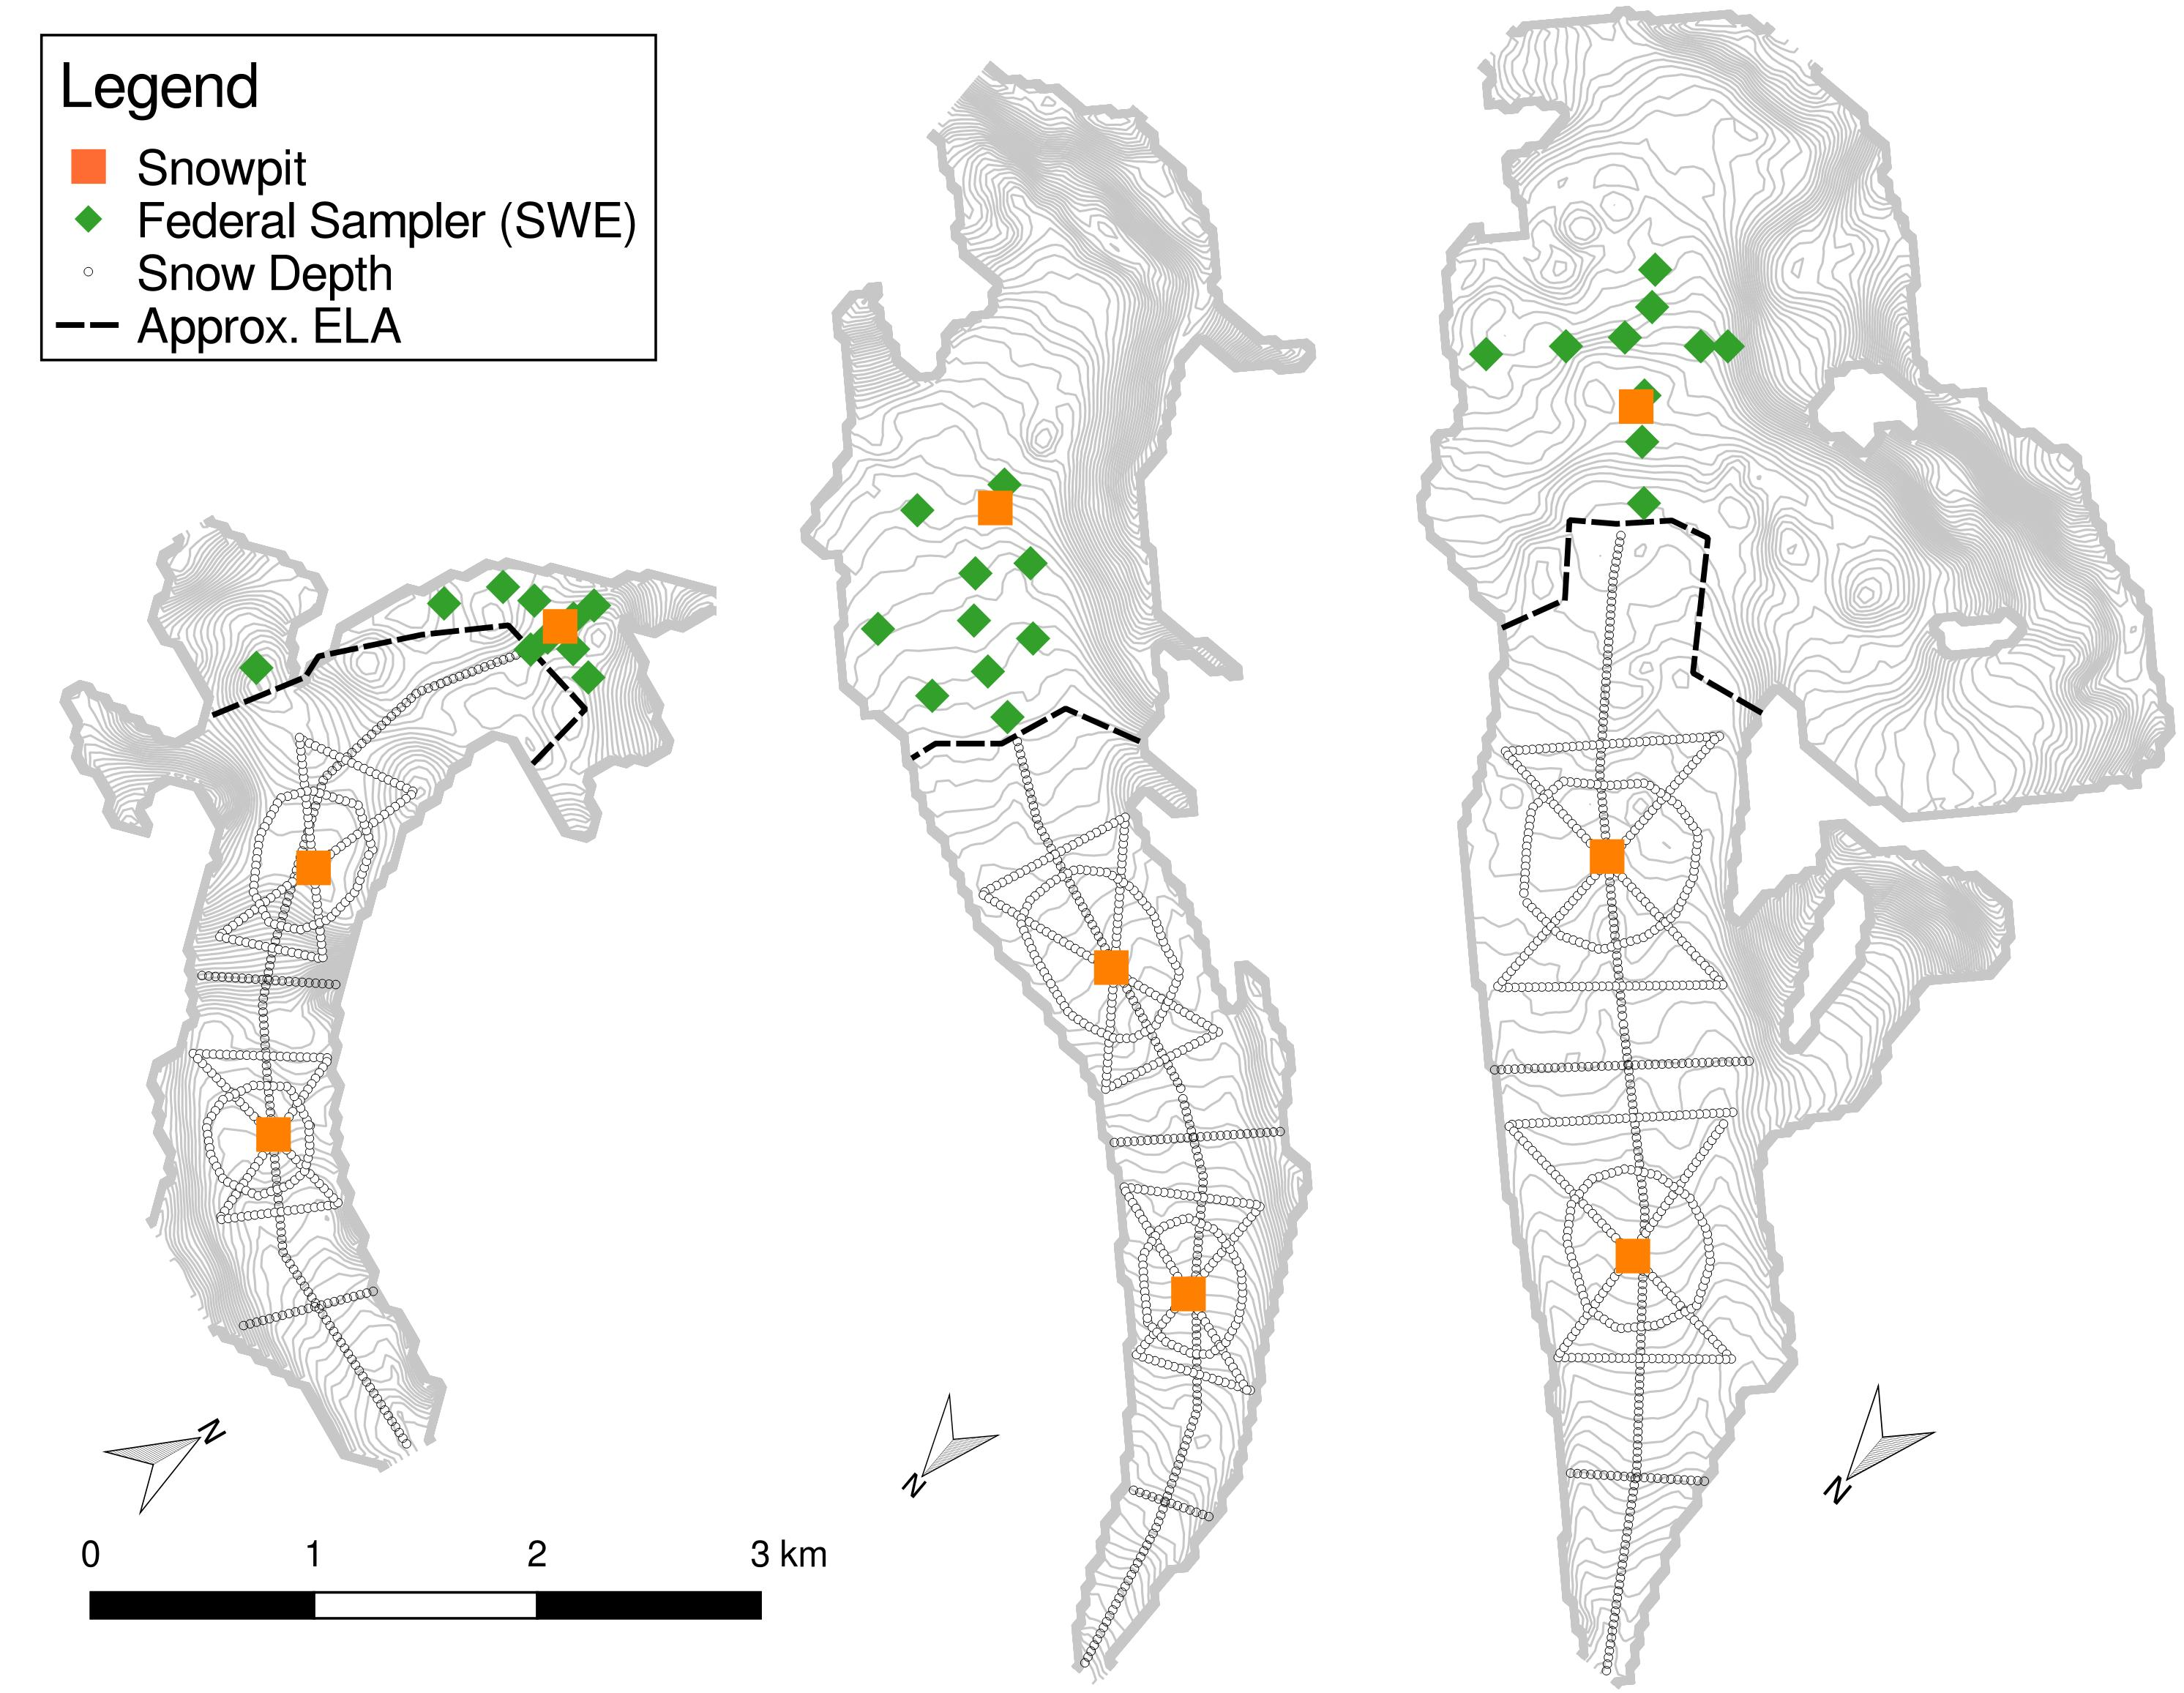
\includegraphics[height = 0.95\textwidth]{Transects_planned.jpeg}}\\
	\caption{Target waypoints for snow depth transects, snow pits, and SWE measurements on three study glaciers.}
	\label{transect_planned}
	\end{figure}

\begin{figure}
	\centering
	\fbox{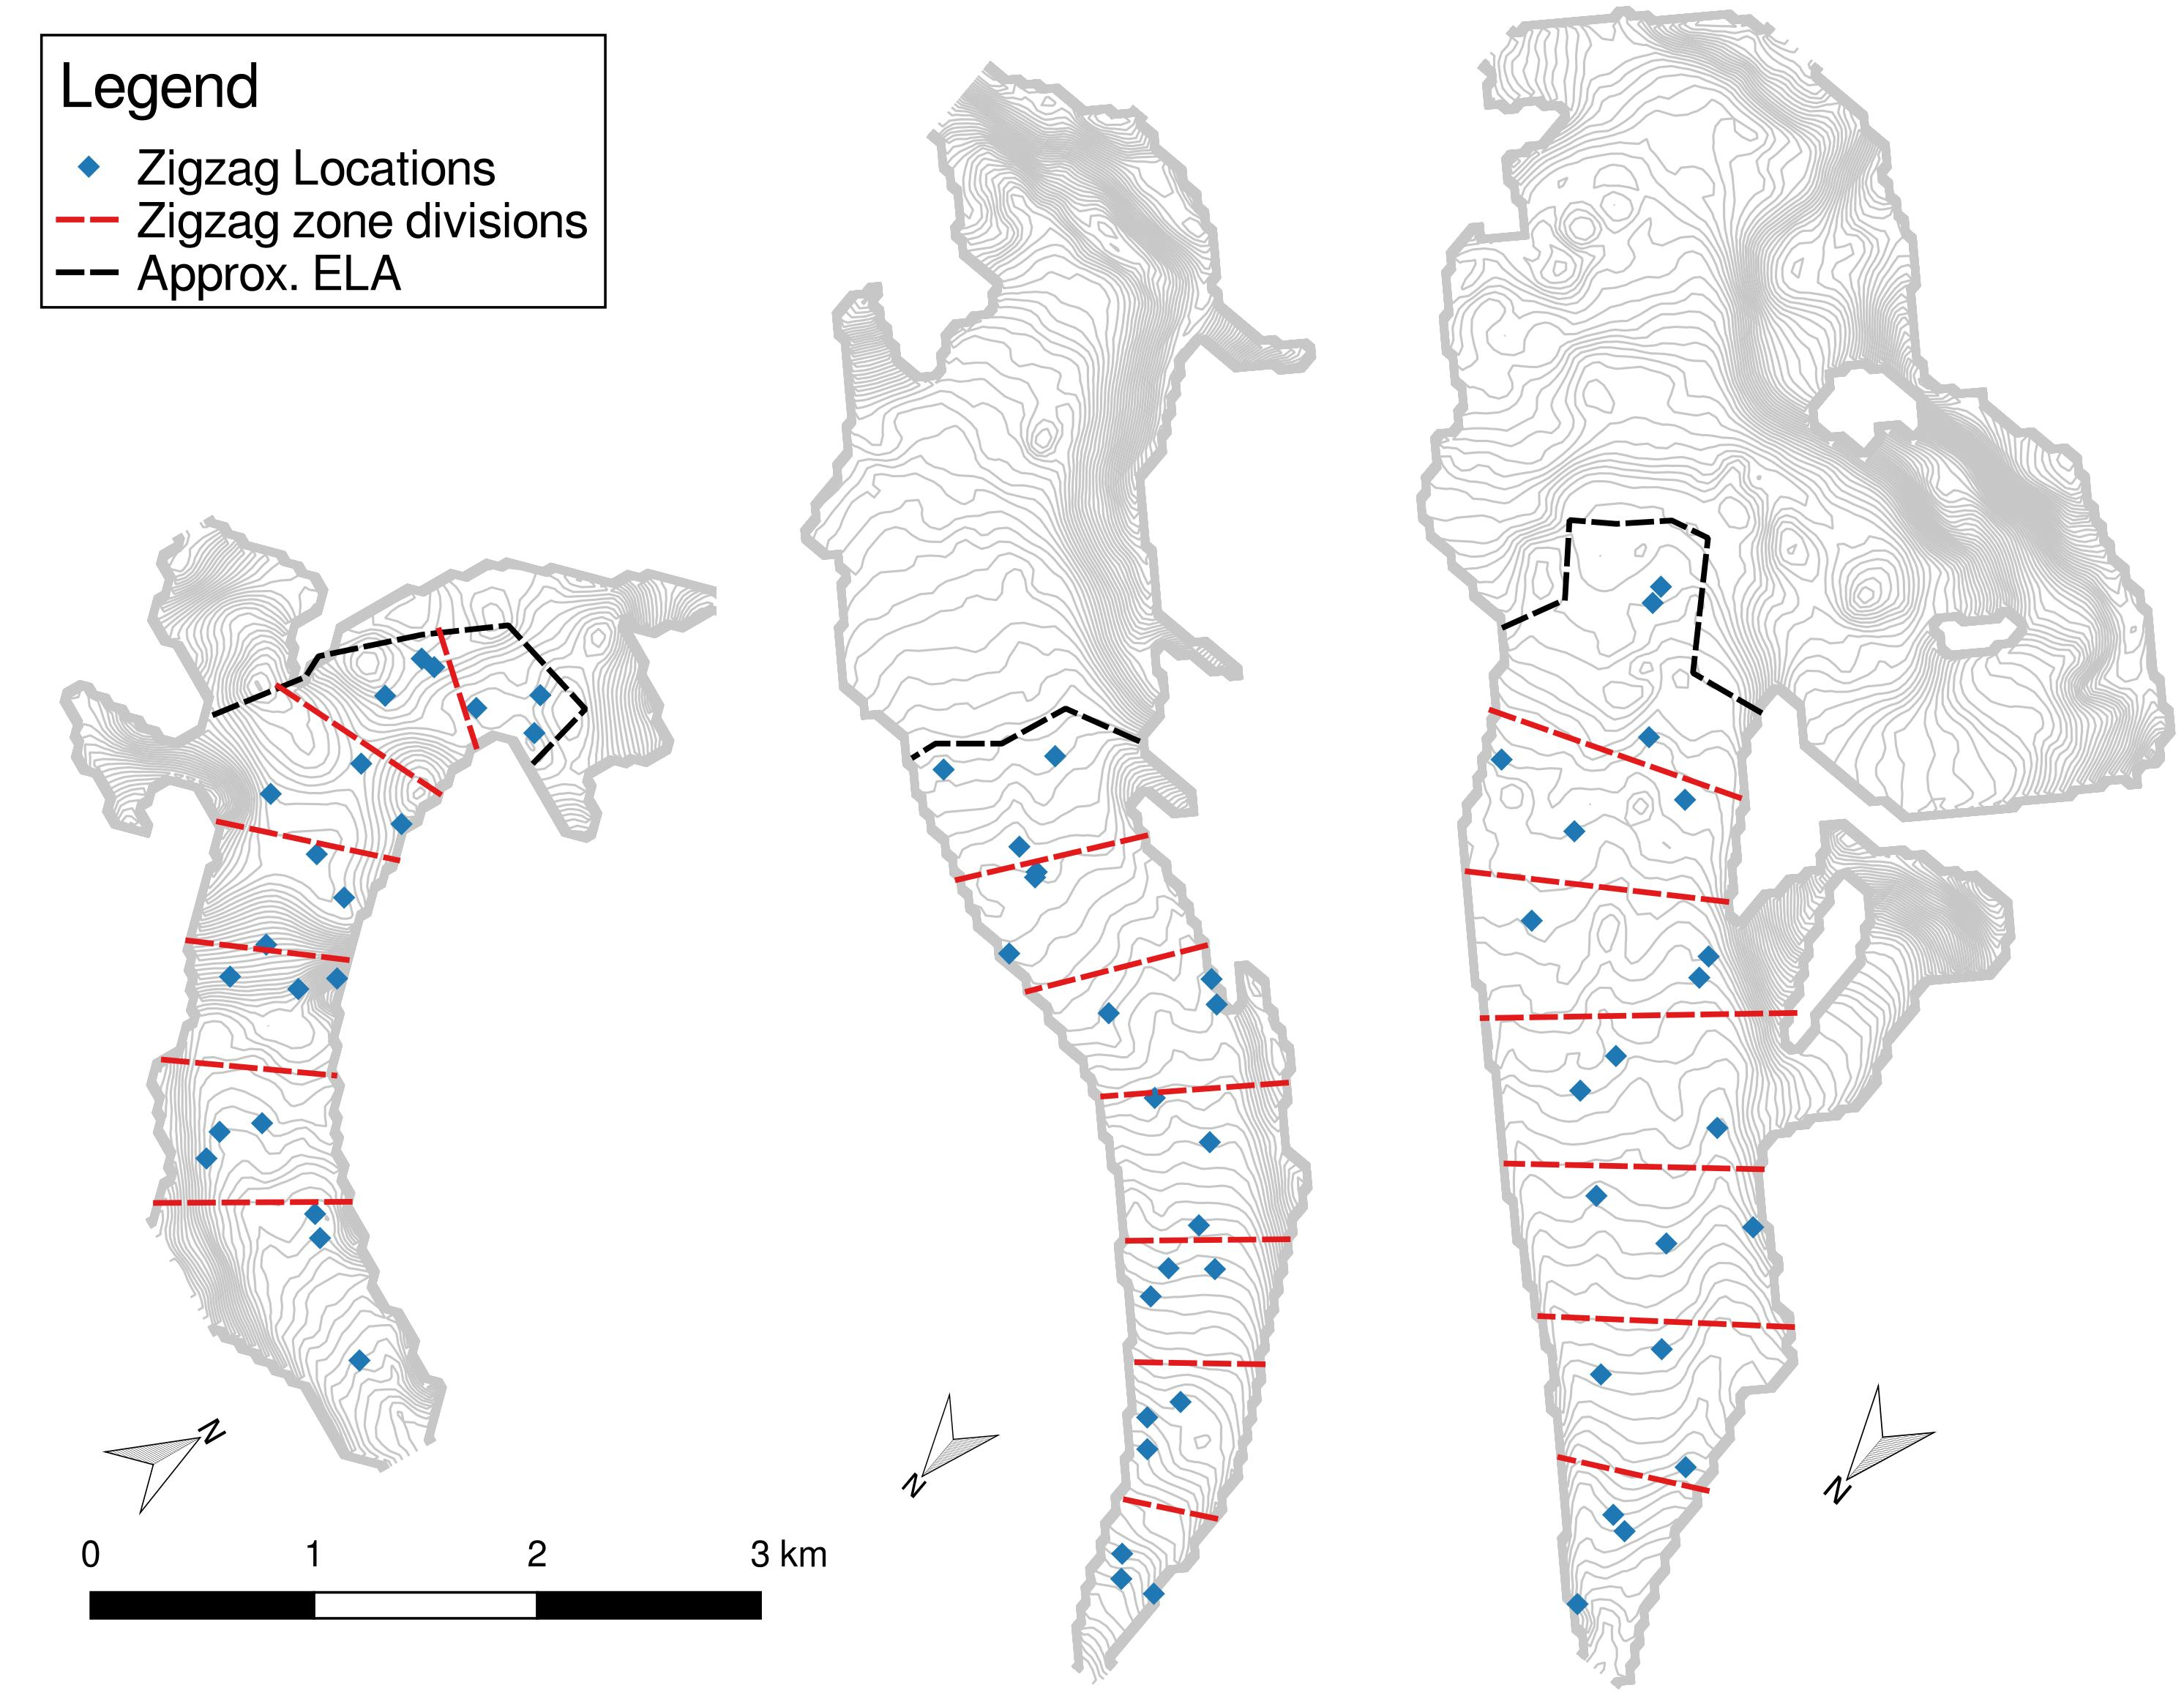
\includegraphics[height = 0.95\textwidth]{Zigzag_planned.jpeg}}\\
	\caption{Randomly assigned locations for zigzag measurements in the ablation area (divided into seven zones).}
	\label{zigzag_planned}
\end{figure}
\end{landscape}

\begin{figure}
	\centering
	\fbox{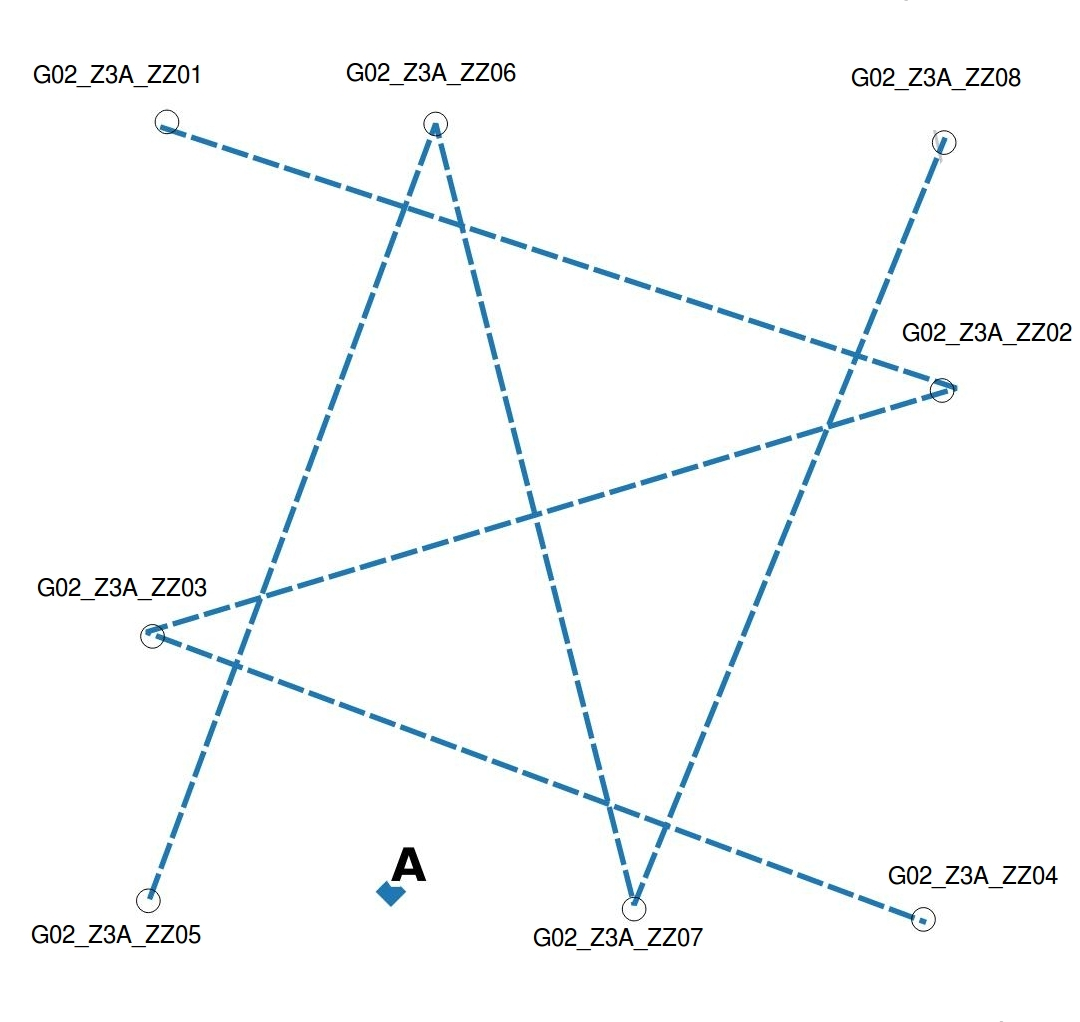
\includegraphics[height = 0.95\textwidth]{ZZ_vertex.jpeg}}\\
	\caption{Example of zigzag. Vertices are labelled and measurements are taken at random intervals along the dashed lines between vertices. The randomly chosen location of the SWE measurement is shown as a diamond.}
	\label{zigzag_vertex}
\end{figure}


\subsection{Waypoint Creation and Upload to GPS Device}

To create the desired \textbf{transect} waypoints and enter them into the handheld GPS devices (Garmin GPSMAP 64s) the following steps were taken:
\begin{enumerate}
\item In QGIS, the outline of the glacier was selected from the Randolph Glacier Inventory (RGI 5.0) \citep{Pfeffer2014} and a recent, end-of-summer Landsat image was downloaded (LC80620172013248LGN00 image courtesy of the U.S. Geological Survey). 
\item The ELA was estimated by tracing out the snow line from the Landsat image.
\item The desired transects were traced out in QGIS within the intended area. The tool `QChainage' was then used to divide the line into points that were spaced every 30 m. Note that the shape file of the transect lines was projected into UTM coordinates to space points using units of metres. 
\item The new point file was then saved as a comma-separated value file (`.csv') and opened in Excel. Note that the projection of the file was WGS84 so that the exported file had latitude and longitude values, which were needed for the GPS software.
\item The points were then named according to their location, area, transect, and point order. A column was made for `Glacier' and `Transect' and filled in for each point (using the drag function in Excel). This required identifying the range of points in QGIS (which were numbered) that corresponded to each transect and relating them to the numbered points in the Excel file (this was a bit cumbersome). The two columns were then combined and a sequential number added to the end. This column requires the header 'name' to be correctly identified as the name of the point in the GPS software.
\item The file with the point names was then imported into to the Garmin software \textit{BaseCamp} and the waypoints were transferred to the GPS devices using this software. 
\end{enumerate}

To create the desired \textbf{zigzag} waypoints and enter them into the GPS devices the following steps were taken:
\begin{enumerate}
\item As described above, the outline of the glacier was selected from the RGI and a recent, end-of-summer Landsat image was downloaded. The ELA was estimated by tracing out the snow line from the Landsat image.
\item The ablation area was then divided into 7 zones that had approximately equal area (estimated by eye) and a polygon was traced out for each zone (within one shape file). 
\item In QGIS, the tool `Random Points' was then used to choose three random locations in each polygon. This was the location of the SWE measurements A, B, and C in each zone. 
\item The file with the SWE measurement locations was saved as a `.csv'. The points were then named in Excel and exported to the GPS device as described above.
\item A new shape file was then created for the vertices of the zigzag. The vertices were created (in sequential order) so that they fit along the edges of one cell of the SPOT5 DEM. This was done by actually looking at one cell and placing the points along the edges at the intended locations. As a result, the SWE measurement location within the zigzag was not the same between zigzags. 
\item Once all the zigzag point groups were created, the file was saved as a `.csv', points named accordingly, and then exported to the GPS device as described above. 
\end{enumerate}

The locations of snowpits and snow cores were chosen by hand in a separate shape file. This file was then saved as a `.csv', the points named, and the file exported to the GPS devices as described above. 

The files that had the names of the points were then imported back into QGIS so that the maps with point labels could be created.  Since the order of completing measurements was determined in the field, these maps helped to quickly decide on the most efficient plan because they aided in determining the relative location of zigzags and transects.

%%%%
\section{Implementation}
%%%%

\subsection{Transects}
\label{sec:transects}

The transects, which include the hourglass, circle, transverse transect, and midline, were all executed in a similar way. Along each transect, waypoints were marked every 30 m. To sample these locations, a team of four people was used in the configuration shown in Figure \ref{photo_probing} and schematically in Figure \ref{probing}. The four people were roped together so that during typical glacier travel there was approximately 10 m separating each person (likely ranged between 9.5 and 11 m). The front person was responsible for navigation and waypoint marking and would follow these steps for each measurement location:
\begin{enumerate}
\item Use the GPS device to locate each intended waypoint
\item Navigate to that location using the GPS device
\item Stop and inform the team when they had arrived at the location
\item Mark a new waypoint on the GPS device as the real location of the measurement (allow for auto labelling of waypoint, which was a three digit number that increased by one with subsequent waypoints). When needed, call out the waypoint label to the team.
\item In one line of a field book, write the labels `Intended' for the waypoint that was being navigated to (code created during planning stage), `Real' for the name of the newly created waypoint on the GPS device (three digit number), as well as the easting, northing, and elevation for that location. This served as the backup for locating measurement points in the event of GPS device failure. 
\end{enumerate}

The remaining three people took snow depth measurement using a graduated 3.2 m avalanche probe. Upon arriving at the waypoint they would follow these steps:
\begin{enumerate}
\item Insert the probe into the snow until the snow/ice interface was reached. Read the depth of the snow pack on the probe to 0.5 cm. Repeat two (or three) more times (total of three (or four) measurements) within a 1 m$^2$ area of the first measurement and in a way that the three (or four) measurements are approximately equidistant. 
\item In one line of a field book, record the `Real' waypoint label (three digit number), as well as the three (or four) depth measurements. 
\end{enumerate}
Note that the snow/ice interface could often be differentiated from an ice lens. Typically, glacier ice felt hard, had a thin, low density (empty feeling) layer above, and created a bright `ping' sound in the probe. Ice lenses felt sticky and the probe would make a dull `thud' sound. In some locations this differentiation was obvious while in other locations it was difficult to be determine what was at the end of the probe. Often, layers in the snowpack could be felt with the probe. For example, the probe would move easily through low density layers such as depth hoar and would `stick' to hard layers or ice lenses. Increasing the force applied to the probe would usually allow the probe to penetrate through hard layers. In cases where the `sticky' layer could not be penetrated, the observer would place a question mark next to the recorded depth or simply omit that measurement. A question mark was also placed beside measurements that were notably smaller than adjacent measurements, which suggested much deeper snow. Note that the probe was inserted vertically, which was not necessarily perpendicular to the snow surface.

It was originally planned for each observer to take four depth measurements in a square pattern. However, during the first transect the observers found time consuming and difficult to remember and record four depths. The observers found that the most efficient way to collect data was to take three depth measurements, remember the values, and then write them all down in the field book. When four measurements were taken it was too difficult to remember all the values simultaneously so the whole process would take much longer. The decision was made to decrease the number of measurements so that we could increase the number of locations measured. 

There were dedicated field books for each type of measurement rather than each observer. The first person had the `Navigation' field book, the second person had `Snow depth \#1', the third person had `Snow depth \#2', and the fourth person had `Snow depth \#3'. In this way, the location of each measured value can be inferred from its location relative to the navigation person (where the location was being recorded). For example, the `Snow depth \#3' value was located $\sim$30 m behind the waypoint location along the trajectory between the previous and current waypoint. This arrangement was preferred to having a field book for each observer because it minimized confusion and potential errors when entering and processing data.

In this arrangement, snow depth measurements could be taken every 10 m along a transect if a waypoint was marked every 30 m. For the first two transects, measurements were completed at every waypoint. However, this also proved to be too time consuming so measurements were taken at every second waypoint for subsequent transects (exceptions include the midline on Glacier 4 and the lower hourglass on Glacier 2, see Table \ref{tab:snowdepthsummary}). A schematic of this arrangement can be seen in Figure \ref{probing:mapview}. Waypoints that were too dangerous to access were omitted. Additional waypoints (not originally uploaded to GPS devices) were created in some instances when travelling from the last accessible waypoint to the next accessible waypoint. A summary of information about the completed snow depth transects can be seen in Table \ref{tab:snowdepthsummary}.

\begin{figure}
	\centering
	\fbox{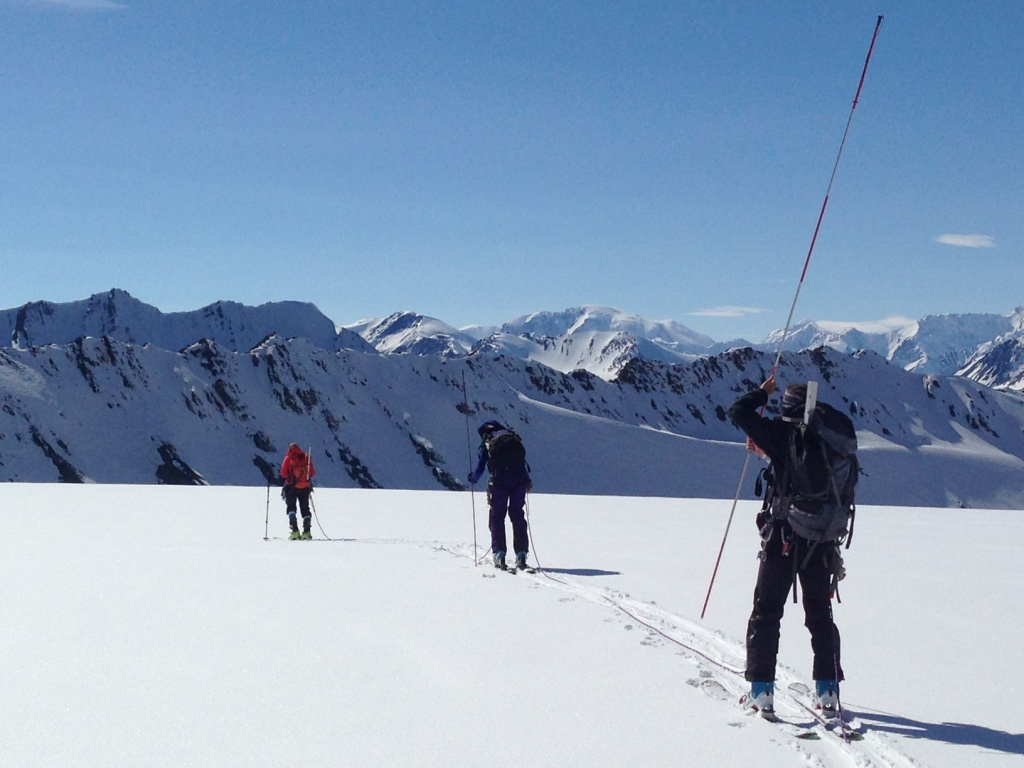
\includegraphics[width = 0.95\textwidth]{photo_probing.jpg}}\\
	\caption{Implementation of transect probing. The first person navigated to the intended waypoint using the GPS device. The second, third, and fourth (not seen) observers are probing using 3.2 m long avalanche probes. There is approximates 10 m between observers. Photo credit: G. Flowers}
	\label{photo_probing}
	\end{figure}


\begin{figure}
    \centering
    \begin{subfigure}[b]{0.8\textwidth}
        \fbox{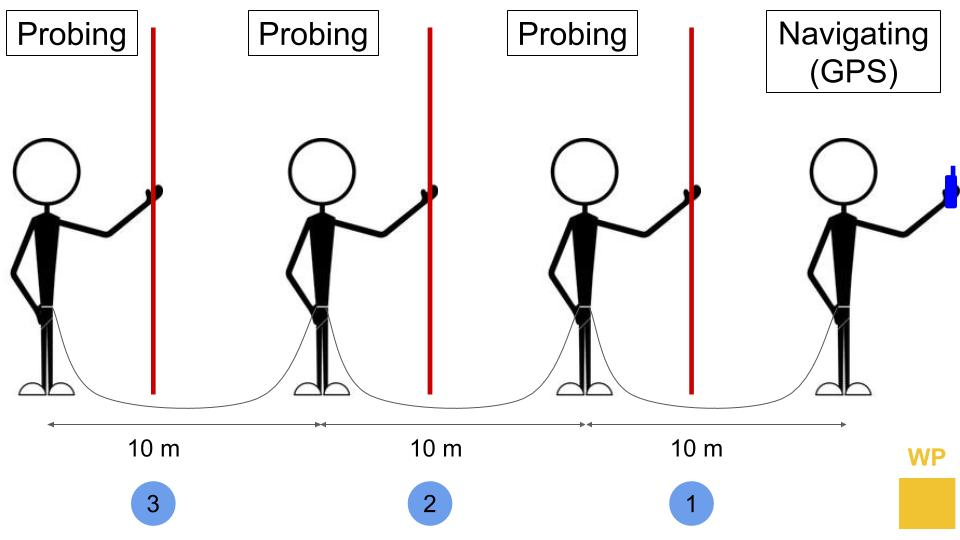
\includegraphics[width=\textwidth]{probers1.jpg}}
        \caption{Relative location of four people taking depth measurements at desired locations.}
        \label{probing:people}
    \end{subfigure}
    
    \begin{subfigure}[b]{0.8\textwidth}
        \fbox{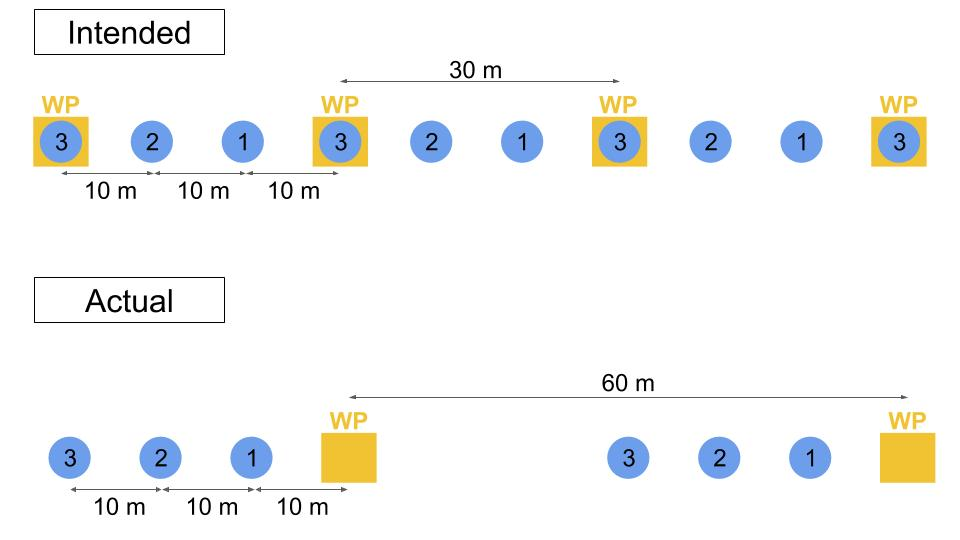
\includegraphics[width=\textwidth]{probers2.jpg}}
        \caption{Intended and actual transect depth measurement spacing. In the intended design, there was continuous measurement with 10 m sampling interval. In the actual implementation, every second waypoint was accessed so there was 60 m between subsequent measurements.}
        \label{probing:mapview}
    \end{subfigure}

    \caption{Schematic of the snow depth measurement configuration. Blue circles indicate depth measurement and orange squares indicate waypoint (WP) location.}\label{probing}
\end{figure}

\begin{landscape}

\begin{table}[]
\footnotesize
\centering
\caption{Summary information for snow depth transects. Transect shapes completed include Lower Hourglass (LH), Lower Circle (LC), Lower Midline (LM), Upper Hourglass (UH), Upper Circle (UC), Upper Midline (UM), Upper Transect (UT), and Bonus Transect (BT). The first observer was navigating to waypoints and the remaining three were taking depth measurements.}
\label{tab:snowdepthsummary}
\begin{tabular}{ccccccl}

\textbf{Glacier}                                                             & \textbf{Shape}                                               & \textbf{\begin{tabular}[c]{@{}c@{}}Measurement\\ Interval\end{tabular}}  & \textbf{Date} & \textbf{\begin{tabular}[c]{@{}c@{}}GPS \\ Waypoint\\  Labels\end{tabular}} & \textbf{\begin{tabular}[c]{@{}c@{}}Observer\\  Order\end{tabular}} & \multicolumn{1}{c}{\textbf{Comments}}                                                                                                                                                                                                            \\ \hline
\multirow{7}{*}{\begin{tabular}[c]{@{}c@{}}Glacier 4\\ (G04)\end{tabular}}   & \textbf{LH}                                                  & \begin{tabular}[c]{@{}c@{}}30 m \\ (60 m for \\ upper part)\end{tabular} & 4 May 2016    & 021 -- 070                                                                 & GF--AP--CA--AC                                                     & \begin{tabular}[c]{@{}l@{}}4 depth measurement/location \\ along upper part\end{tabular}                                                                                                                                                         \\
                                                                             & \textbf{LC}                                                  & 60 m                                                                     & 6 May 2016    & 159 -- 184                                                                 & GF--AP--CA--AC                                                     &                                                                                                                                                                                                                                                  \\
                                                                             & \textbf{LM}                                                  & 90 m                                                                     & 7 May 2016    & 185 -- 207                                                                 & AP--GF--CA--AC                                                     &                                                                                                                                                                                                                                                  \\
                                                                             & \textbf{UH}                                                  & 60 m                                                                     & 5 May 2016    & 072 -- 126                                                                 & CA--GF--AP--AC                                                     &                                                                                                                                                                                                                                                  \\
                                                                             & \textbf{UC}                                                  & 60 m                                                                     & 5 May 2016    & 127 -- 157                                                                 & CA--GF--AP--AC                                                     &                                                                                                                                                                                                                                                  \\
                                                                             & \textbf{UM}                                                  & 90 m                                                                     & 7 May 2016    & 208 -- 221                                                                 & AP--GF--CA--AC                                                     & Additional measurement at WP 158 (6 May 2016)                                                                                                                                                                                                               \\
                                                                             & \textbf{UT}                                                  & 30 m                                                                     & 4 May 2016    & 004 -- 020                                                                 & GF--AP--CA--AC                                                     & 4 depth measurement/location                                                                                                                                                                                                                     \\ \hline
\multirow{7}{*}{\begin{tabular}[c]{@{}c@{}}Glacier 2 \\ (G02)\end{tabular}}  & \textbf{\begin{tabular}[c]{@{}c@{}}LH \\ \& LC\end{tabular}} & 30 m                                                                     & 11 May 2016   & 371 -- 518                                                                 & GF--AP--CA                                                         & \begin{tabular}[c]{@{}l@{}}Only two probers. Avoided crossing main \\ channel so LH \& LC were combined and \\ done together on glacier right and then \\ glacier left of the channel. Almost all \\ measurements in the dune area.\end{tabular} \\
                                                                             & \textbf{LM}                                                  & $\sim$60 m                                                               & 10 May 2016   & 355 -- 370                                                                 & AP--GF--CA--AC                                                     & \begin{tabular}[c]{@{}l@{}}Original points along supraglacial stream \\ bed so points moved to glacier right and \\ locations were approximated\end{tabular}                                                                                     \\
                                                                             & \textbf{UH}                                                  & 60 m                                                                     & 8 May 2016    & 223 -- 275                                                                 & AC--AP--CA--GF                                                     & \begin{tabular}[c]{@{}l@{}}Many corner points avoided due to \\ crevasse danger\end{tabular}                                                                                                                                                     \\
                                                                             & \textbf{UC}                                                  & 60 m                                                                     & 8 May 2016    & 276 -- 313                                                                 & AC--AP--CA--GF                                                     &                                                                                                                                                                                                                                                  \\
                                                                             & \textbf{UM}                                                  & 60 m                                                                     & 9 May 2016    & 313 -- 343                                                                 & AC--AP--CA--GF                                                     &                                                                                                                                                                                                                                                  \\
                                                                             & \textbf{UT}                                                  & 60 m                                                                     & 11 May 2016   & 519 -- 528                                                                 & GF--AP--CA                                                         & Only two probers                                                                                                                                                                                                                                 \\
                                                                             & \textbf{BT}                                                  & $\sim$60 m                                                               & 19 May 2016   & 344 -- 354                                                                 & GF--AP--CA--AC                                                     &                                                                                                                                                                                                                                                  \\ \hline
\multirow{7}{*}{\begin{tabular}[c]{@{}c@{}}Glacier 13 \\ (G13)\end{tabular}} & \textbf{LH}                                                  & 60 m                                                                     & 15 May 2016   & 745 -- 811                                                                 & AC--AP--CA--GF                                                     &                                                                                                                                                                                                                                                  \\
                                                                             & \textbf{LC}                                                  & 60 m                                                                     & 15 May 2016   & 812 -- 847                                                                 & AC--AP--CA--GF                                                     &                                                                                                                                                                                                                                                  \\
                                                                             & \textbf{LM}                                                  & 60 m                                                                     & 14 May 2016   & 714 -- 743                                                                 & AC--AP--CA--GF                                                     &                                                                                                                                                                                                                                                  \\
                                                                             & \textbf{UH}                                                  & 60 m                                                                     & 12 May 2016   & 571 -- 650                                                                 & AC--GF--CA--AP                                                     &                                                                                                                                                                                                                                                  \\
                                                                             & \textbf{UC}                                                  & 60 m                                                                     & 12 May 2016   & 529 -- 570                                                                 & AC--GF--CA--AP                                                     &                                                                                                                                                                                                                                                  \\
                                                                             & \textbf{UM}                                                  & 60 m                                                                     & 14 May 2016   & 678 -- 713                                                                 & AC--AP--CA--GF                                                     &                                                                                                                                                                                                                                                  \\
                                                                             & \textbf{UT}                                                  & 60 m                                                                     & 14 May 2016   & 660 -- 677                                                                 & AC--AP--CA--GF                                                     &                                                                                                                                                                                                                                                 
\end{tabular}
\end{table}

\normalsize
\begin{table}[]
\centering
\caption{Summary information for zigzag measurements}
\label{tab:zigzagsummary}
\begin{tabular}{cccccl}
\textbf{Glacier} & \textbf{Zone} & \textbf{Priority} & \textbf{Date} & \textbf{Observers} & \multicolumn{1}{c}{\textbf{Comments}}                                                                          \\ \hline
G04              & 3             & A                 & 5 May 2016    & AP/CA              &                                                                                                                \\
G04              & 2             & A                 & 7 May 2016    & CA/AC              &                                                                                                                \\
G04              & 5             & B                 & 7 May 2016    & AP/GF              & \begin{tabular}[t]{@{}l@{}}Sticky layer - many points not collected\\ Snowing during measurements\end{tabular} \\ \hline
G02              & 5             & C                 & 10 May 2016   & CA/GF              & \begin{tabular}[t]{@{}l@{}}Extra line measured\\ Vertex labelling error in GPS device \end{tabular}                                                                                   \\
G02              & 7             & A                 & 10 May 2016   & CA/GF/AP/AC              & \begin{tabular}[t]{@{}l@{}}Channel present\\ Vertex labelling error in GPS device\end{tabular}                        \\
G02              & 3             & B                 & 10 May 2016   & GF/AP              & Vertex labelling error in GPS device                                                                                  \\ \hline
G13              & 7             & C                 & 14 May 2016   & AC/AP              & Vertex labelling error in GPS device                                                                                  \\
G13              & 4             & C                 & 14 May 2016   & GF/CA              & \begin{tabular}[t]{@{}l@{}}Channel present\\ Vertex labelling error in GPS device\end{tabular}                        \\
G13              & 3             & B                 & 15 May 2016   & GF/CA              & Vertex labelling error in GPS device                                                                                  \\
G13              & 5             & A                 & 15 May 2016   & AP/AC              & \begin{tabular}[t]{@{}l@{}}Mushy snow that collapses\\ Vertex labelling error in GPS device\end{tabular}             
\end{tabular}
\end{table}

 \begin{figure}
	\centering
	\fbox{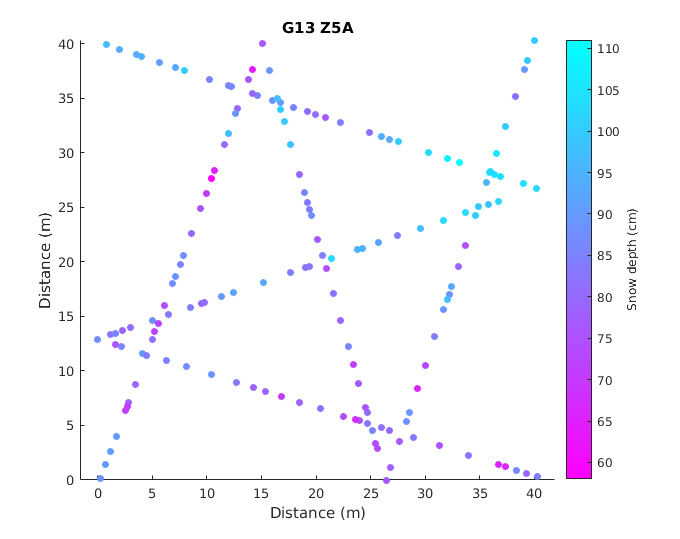
\includegraphics[height = \textwidth]{zigzag_completed.png}}\\
	\caption{Snow depth values measured along a zigzag pattern (G04\_Z3A)}
	\label{zigzag_example}
\end{figure}

\end{landscape}

\begin{table}[]
\centering
\caption{Summary information for SWE measurements with the Federal Snow Sampler}
\label{tab:SWEsummary}
\begin{tabular}{ccccccl}
\textbf{Glacier}      & \textbf{Location} & \textbf{\begin{tabular}[c]{@{}c@{}}Total\\ Values\end{tabular}} & \textbf{\begin{tabular}[c]{@{}c@{}}Number \\ of Tube \\ Lengths\end{tabular}} & \textbf{Date} & \textbf{Observers} & \multicolumn{1}{c}{\textbf{Comments}}                                        \\ \hline
\multirow{7}{*}{G04}  & Z3A               & 5                                                               & 3                                                                             & 5 May 2016    & GF/AC              &                                                                              \\
                      & USP               & 2+2+2+3                                                         & 3                                                                             & 5 May 2016    & GF/CA              &                                                                              \\
                      & Z2A               & 3                                                               & 3                                                                             & 7 May 2016    & GF/AP              &                                                                              \\
                      & LSP               & 3+2+2+2                                                         & 3                                                                             & 7 May 2016    & GF/CA              &                                                                              \\
                      & Z5B               & 3                                                               & 3                                                                             & 7 May 2016    & CA/AC              &                                                                              \\
                      & Z5A               & 3                                                               & 3                                                                             & 7 May 2016    & CA/AC              &                                                                              \\
                      & Z5C               & 3                                                               & 2                                                                             & 7 May 2016    & CA/AC              &                                                                              \\ \hline
\multirow{7}{*}{G02}  & Z5C               & 3                                                               & 2                                                                             & 10 May 2016   & AP/AC              &                                                                              \\
                      & USP               & 3+2+2+2                                                         & 2                                                                             & 10 May 2016   & AP/AC              &                                                                              \\
                      & Z7A               & 3                                                               & 3                                                                             & 10 May 2016   & CA/GF              &                                                                              \\
                      & Z7B               & 3                                                               & 3                                                                             & 10 May 2016   & CA/GF              &                                                                              \\
                      & Z7C               & 3                                                               & 2                                                                             & 10 May 2016   & AP/CA              &                                                                              \\
                      & LSP               & 2+2+2+2                                                         & 1                                                                             & 10 May 2016   & CA/AC              & \begin{tabular}[t]{@{}l@{}}Used snowpit \\ spring scale (grams)\end{tabular} \\
                      & Z3B               & 3                                                               & 1                                                                             & 10 May 2016   & CA/AC              & \begin{tabular}[t]{@{}l@{}}Used snowpit \\ spring scale (grams)\end{tabular} \\ \hline
\multirow{19}{*}{G13} & ASP               & 2+2+2+2                                                         & 3                                                                             & 13 May 2016   & AP/AC              &                                                                              \\
                      & AFC05             & 3                                                               & 3                                                                             & 13 May 2016   & AP/CA              & \begin{tabular}[t]{@{}l@{}}Probe depth \\ $\neq$ tube depth\end{tabular}     \\
                      & WP 651            & 3                                                               & 3                                                                             & 13 May 2016   & AP/CA/GF           &                                                                              \\
                      & WP 652            & 4                                                               & 3                                                                             & 13 May 2016   & AP/CA/GF           &                                                                              \\
                      & WP 653            & 3                                                               & 3                                                                             & 13 May 2016   & AP/CA/GF           &                                                                              \\
                      & WP 654            & 3                                                               & 3                                                                             & 13 May 2016   & AP/CA/GF           &                                                                              \\
                      & WP 655            & 3                                                               & 3                                                                             & 13 May 2016   & AP/CA/GF           &                                                                              \\
                      & WP 656            & 3                                                               & 3                                                                             & 13 May 2016   & AP/CA/GF           &                                                                              \\
                      & WP 657            & 3                                                               & 3                                                                             & 13 May 2016   & AP/CA/GF           &                                                                              \\
                      & WP 658            & 3                                                               & 3                                                                             & 13 May 2016   & AP/CA/GF           &                                                                              \\
                      & WP 659            & 3                                                               & 3                                                                             & 13 May 2016   & AP/CA/GF           &                                                                              \\
                      & Z7C               & 3                                                               & 2                                                                             & 13 May 2016   & CA/GF              &                                                                              \\
                      & USP               & 2+2+2+2                                                         & 2                                                                             & 14 May 2016   & AP/AC              & \begin{tabular}[t]{@{}l@{}}Ice layer near \\ bottom\end{tabular}             \\
                      & Z4C               & 3                                                               & 3                                                                             & 14 May 2016   & AP                 & In stream channel                                                            \\
                      & WP 744            & 3                                                               & 2                                                                             & 14 May 2016   & AP                 & In Z4C zigzag                                                                \\
                      & Z3B               & 3                                                               & 2                                                                             & 15 May 2016   & AP/AC              &                                                                              \\
                      & Z4B               & 3                                                               & 2                                                                             & 15 May 2016   & AP/AC              &                                                                              \\
                      & Z5C               & 3                                                               & 2                                                                             & 15 May 2016   & CA/GF              &                                                                              \\
                      & Z5B               & 3                                                               & 2                                                                             & 15 May 2016   & CA/AC              &                                                                             
\end{tabular}
\end{table}



\subsection{Zigzag}

The zigzag sampling pattern was used to obtain many measurements within a 40 x 40 m area.  The pattern consisted of two intersecting `Z' shaped transects. Snow depth was measured with random spacing between 0.3 m and 3.0 m. 

Two teams of two people were used to complete each zigzag. The first team would navigate to the vertices of the zigzag using the GPS device and place wands at each vertex. Often the tracks would not be straight between two vertices so the second team would use the wands to travel between vertices in as straight a line as possible. The first person would use the avalanche probe to measure out the distance to the next measurement spot and then probe at that point (Sturm, M., 2016 personal communication). Probing protocol was exactly the same as for transect measurements (see Section \ref{sec:transects}). The first person would call out the depth to the second person, who was responsible for recording the distance between measurements and the depth at the measurement point. A field book was dedicated to zigzag measurements and each page would have the name of the vertex where measurements started, the distance from the previous measurement point and the depth at that point. The second person also had a sheet with random numbers from a uniform distribution between 0.3 and 3.0 m (generated used Matlab) and would call out these numbers in order as the distance between measurement points. While the second team was measuring snow depth, the first team took three SWE measurements with a $\sim$1 m area around the predetermined location within the zigzag area (see Section \ref{sec:SWE} for protocol). An example of a completed zigzag pattern can be seen in Figure \ref{zigzag_example} and a summary of information about completed zigzags can be seen in Table \ref{tab:zigzagsummary}.


 \subsection{Federal Snow Sampler}
\label{sec:SWE}
 
\begin{figure}
    \centering
    \begin{subfigure}[b]{0.38\textwidth}
        \fbox{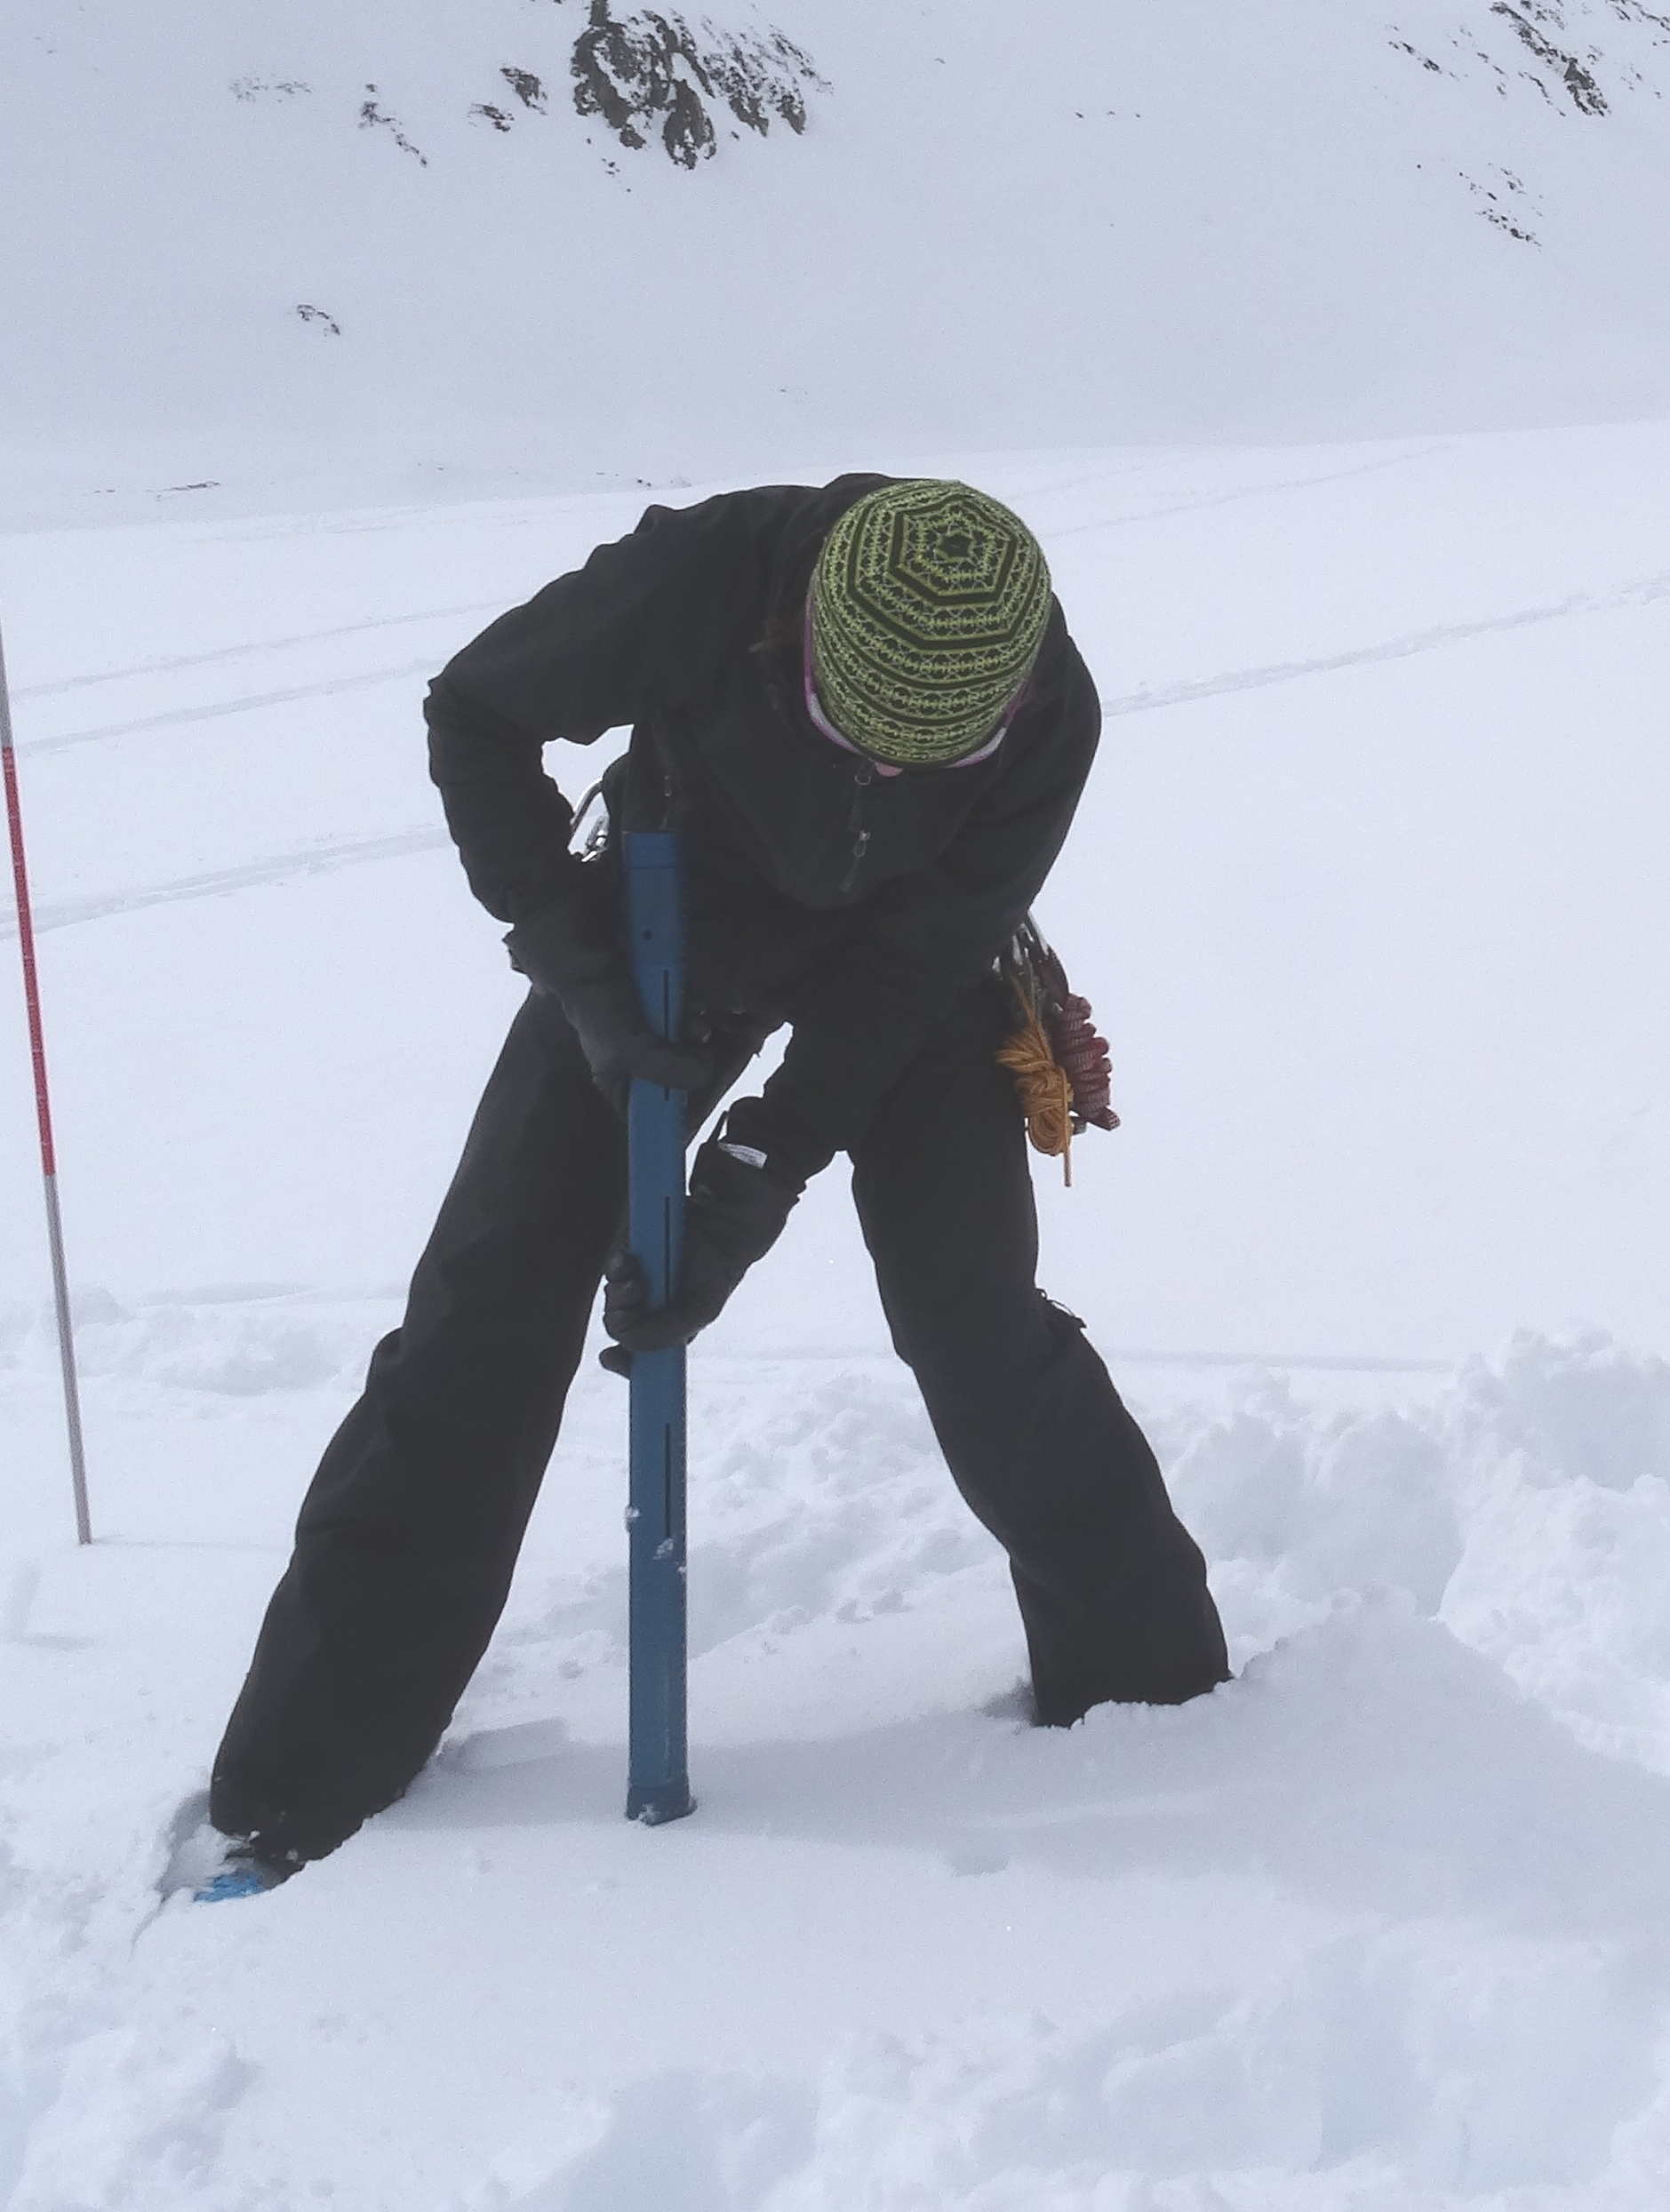
\includegraphics[width=\textwidth]{photo_swe1.JPG}}
        \caption{Inserting the Federal Sampler into the snow. Photo credit: C. Ariagno}
        \label{photo_swe1}
    \end{subfigure}
    ~
    \begin{subfigure}[b]{0.56\textwidth}
        \fbox{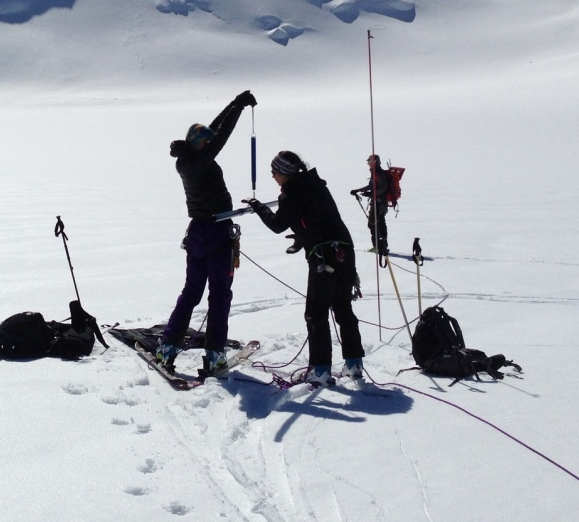
\includegraphics[width=\textwidth]{photo_swe2.jpg}}
        \caption{Weighing the Federal Sampler with snow core on the spring scale (units of cm SWE).Photo credit: G. Flowers}
        \label{photo_swe2}
    \end{subfigure}

    \caption{Using the Federal Sampler to measure SWE}
    \label{photo_swe}
\end{figure}
 
A metric Federal Snow Sampler from Geo Scientific Ltd. was used to measure snow depth and snow water equivalent (SWE). At the predetermined locations, three measurements (within 50 cm of each other) were made using the sampler. At the snowpit locations, a total of eight measurements were made, with two measurements on each side of the snowpit. Density calculated from these values will be compared with density determined from sampling within the snow pit (see Section \ref{sec:snowpit}). 

The Federal Snow Sampler consists of four 0.83 m sections that could be screwed together. One end of the sampler has cutter teeth and the other end has a removable thread protector that can be screwed onto the top section of the tube. The sampler has graduations in units of 1 cm and slits along the side of the tube allow the observer to determine the length of the core when it is in the tube. The spring scale that comes with the Federal Sampler is in units of cm SWE.  

To take a measurement with the Federal Sampler the following steps were taken:
\begin{enumerate}
\item Three depth measurements (within $\sim$50 cm of each other) were made using an avalanche probe and the depths were recorded.
\item The weight (in cm SWE) of the assembled empty tube was measured using the spring scale and then recorded (tare).
\item The tube was placed vertically into the snow and then pushed and twisted clockwise so that the cutters at the end of the tube would penetrate the snow pack. If this proved to be too difficult, the T-handle was added onto the tube to aid in pushing the tube further into the snow. 
\item When the bottom of the snow pack was reached, the observer would measure the snow depth by using the graduation on the outside of the tube.
\item The tube was then gently pulled out of the snow (so as not to lose any snow from the bottom). The length of the snow core inside the tube was then measured by using the side slits to see the top of the core and lining it up with the graduation on the outside of the tube. This value was then recorded. If the length of the snow core was much less than the snow depth (typically a result of lost snow), the sample measurement was redone.
\item The snow and tube were weighed together using the spring scale and the value was recorded.
\item The tube was then emptied and wiped using a soft cloth on a pole to remove any moisture. 
\end{enumerate}

When the T-handle was used, the tube segments often became difficult to take apart. The small handles provided in the kit aided in disassembling the Federal Sampler. However, if a significant force was applied to the T-handle during sampling and the tube segments seized then longer handles (accomplished by attaching snow shovel handles to provided tools) helped in disassembling the sampler. Anti-seizing compound was included in the kit and was applied when needed. A summary of information about completed SWE measurements can be seen in Table \ref{tab:SWEsummary}.

\subsection{Firn Corer}

The firn corer was intended to be used in the accumulation area to extract a snow/firn core. The coring device would be beneficial in the accumulation area because the core can be extracted and used to determine the location of the snow/firn transition. From that, the snow depth and the mass of the snow core, which included only the past year of accumulation, could be determined. The Federal Sampler was thought to be ineffective in the accumulation area because the snow/firn transition may not have been felt and the core cannot be examined to establish where the transition occurs.

When the corer was used in the field however, a number of problems were encountered that prevented the collection of accurate measurements. The first was that the snow core would get stuck inside the core barrel. Warm temperatures meant that the barrel would get wet from snow melt and when it was inserted into the snow pack, the snow would freeze onto the side of the barrel. This meant that the core was destroyed in the extraction process. The second problem (which was connected to the first problem) was that the coring chips in the hole could not be discriminated from the core itself. Coring chips are loose snow crystals that fall to the bottom of the drilling hole when the barrel is taken out. When the barrel is reinserted for the second (or third) core, the snow in the subsequent core will contain these coring chips, which are not part of the intended core. The mass of the core will be incorrect (overestimate) because of this additional snow. This problem is typically avoided by extracting the in-tact core and identifying and removing the coring chips. However, since the core could not be extracted as one piece, this step was not possible and the masses of the cores were incorrect. 

In a few locations, sections of the core could be exacted without breaking them apart. In these areas the snow/firn transition could be identified. This means that in principal, the firn corer could be used to determine the depth of this transition. The main challenge is therefore being able to identify chips. In firn core trials that occurred after this field work, it was found that the the cores could be pulled out easily if the barrel was not totally full. However, in these less compacted cores the chips were difficult to identify so the problem persists. 

As a result of these complications, many accumulation area measurements on Glacier 4 and Glacier 2 were abandoned. On Glacier 13, the Federal Sampler was successfully used to take SWE measurements. The snow/firn transition could be felt with the Federal Sampler because of the large density change, which made it almost impossible to further insert the tube into the snow pack.  

\subsection{Snowpit}
\label{sec:snowpit}


Three snowpits were excavated on each glacier and snow density sampled every 10 cm using a wedge cutter (Snow Metrics RIP 2 Cutter (250 cc)). The snow temperature was also measured at 10 cm intervals. The snowpit was oriented so that the sampling face was in the shade (typically south edge of snowpit), which reduces melt. 

The measurement procedure in the snowpit was as follows:
\begin{enumerate}
\item The face of the wall that was chosen for sampling was smoothed and a ruler was placed against the wall with the 0 cm mark at the bottom of the snowpit. The ruler was used to measure sampling heights within the snow pack. The snow surface directly above this wall was undisturbed during the digging process so that the true snow depth could be determined. 
\item Air and snow surface temperature were measured by placing the thermometer (dial-stem thermometer ($\pm$0.5$^\circ$)) in the shade of a shovel or ski. 
\item A snow density sample was taken in 10 cm intervals through the full depth of the snow pack. Samples were offset horizontally from each other so that the snow was not affected by previous measurements. 
	\begin{enumerate}
	\item The wedge cutter was inserted into the snow vertically (to sample 10 cm intervals) and the top was slid onto the wedge to isolate the sample. The wedge was taken out and inspected. If the sample appeared to fill the entire wedge (no obvious voids) then the wedge was emptied into a small plastic bag. If the sample was poor then the snow was discarded and a new sample was taken at the same height in the snow pit. 
	\item A spring scale ($\pm$2.5 g) was then used to weigh the bag with the snow sample and the weight was recorded. The snow sample was then discarded. Note that the spring scale was tared with an empty bag.
	\end{enumerate}
\item Snow temperatures were also measured and recorded every 10 cm. The thermometer was inserted into the snow at the desired location and left to equilibrate for several minutes. The temperature was then recorded.
\end{enumerate}

Modifications to this procedure occurred when snow samples could not be taken because the snow was too dense. This would often occur when ice layers or lenses were present in the snow, which could not be cut by the wedge. In these cases, the measured thickness was recorded. A sample would then be taken using the wedge cutter but aligned horizontally so that a 5 cm tall sample was taken. Additionally, the sample interval closest to the ice surface (0--10 cm) would be difficult to obtain because the ice was rough and the snow above was faceted. Sometimes, this sample could not be obtained or a 5 cm sample needed to be taken. 

After the majority of snowpit measurements were completed, a spring scale with finer resolution was found. For Glacier 4 and 2 the coarse resolution (10 g) scale had been used but for Glacier 13 the fine resolution (2 g) scale was used. Future measurements should use the finer resolution spring scale when using the small wedge sampler. As a result, the snow-density uncertainty is larger for Glacier 4 and 2 than for Glacier 13. 

\begin{figure}
	\centering
	\fbox{\includegraphics[width = 0.95\textwidth]{photo_snowpit.jpg}}\\
	\caption{Taking snow denisty measurements in a snowpit. An expandable ruler is used to measure snow depth and determine sampling locations. A 250cc wedge cutter is used to extract a known volume of snow and a spring scale is used to weigh the snow. The dial-stem thermometer is used for measureing snow temperature. Note that the sampling wall is shaded, has an undistrubed snow surface above it, and has a smoothed face. Photo credit: A. Criscitiello}
	\label{photo_snowpit}
	\end{figure}
	
%%%%
\section{Daily Synopsis}
%%%%

\textbf{People}: Gwenn Flowers, Alex Pulwicki, Coline Ariagno, Ali Criscitiello

\noindent \textbf{Dates}: April 30 -- May 3 (KLRS), May 4 -- May 8 (Glacier 4), May 8 -- May 12 (Glacier 2), May 12 -- May 16 (Glacier 13)

\subsection{Pre-trip}

\textbf{SFU}

Coline prepared the food spreadsheet and Alex and Coline bought food. Alex brought most of the gear to AirNorth shipping on April 28th. All other pre-trip items tasks were accomplished. 

\noindent \textbf{KLRS}

Flew in to Whitehorse on April 30th. Picked up rental van and our shipped gear. Everything and everyone arrived safe and sound. We had a total of 3 full days at the station to complete tasks. Bonus tasks that were done included rigging the tents and updating box inventory (Coline).

\subsection{Glacier 4}

\textbf{Camp and logistics}

We had a lot of gear and the helicopter only had one ski basket so packing was challenging. Dion was able to shut down each time, which helped considerably. We did manage to squeeze in but the back of the helicopter was quite packed. Dion said that we are likely at the weight limit for the helicopter at that altitude. Overall, flight in was good.

Camp was set up with four tents in a square formation and a megamid to the south. Moraine was windy so exposed rocks were present. The snow was not quite deep enough to properly dig out the inside of the megamid. Next time, it would be good to probe around to find deeper snow so that the inside is more comfortable. Cooking in the megamid was great both in the morning and evening. We would collapse the tent during the day and at night. When it snowed or there was blowing snow the collapsed tent would accumulate snow and it was hard to take the snow off without damaging the shell with the shovel. We did put a number of small holes in the material. Maybe it would be good to bring a small plastic shovel next time? Also, the megamid would benefit from a snow skirt so that it would be easier to put snow along the edges. We used wooden dowels for snow stakes and it worked well --- bring more next time if possible. We sat on foamies inside the megamid and that worked well as well. Gwenn bought more snow stakes so each MEC tent had 5--6 stakes and that worked well.

\vspace{4mm}
\noindent \textbf{General Science Notes}

Accumulation seems to be strongly affected by wind. Margins have some areas with a lot of scour while other areas have very deep snow that is likely from preferential deposition/redistribution. The centre of the glacier seems to be relatively uniform and varies smoothly. 

GPS device (Garmin GPSMAP 64s, bought 2016) is working very well for navigation. All the waypoints were entered correctly and it's relatively easy to find them. We can zoom into an area with the cursor and then search closest to that to locate the intended waypoint. The paper maps with zigzag locations and transects were incredibly valuable for deciding what we wanted to and in which order as well as knowing where to look on the GPS device for an intended waypoint. Most useful pages were the zigzag one and the everything combined one although, all were used in the end. 

Terrain of Glacier 4 does not match the SPOT5 DEM (especially in the middle `steep' part, which did not exist). What does this mean for the regression with topographic parameters?

Crevasses were seen on glacier right and middle on the ramp up to the upper plateau/accumulation area and some large features in the upper plateau. One large feature had a large, steep wall facing up glacier (maybe a lake?).

It snowed a number of times during this part of the trip. It would have been good to have a snow board on the glacier (not at camp because we were in a scoured area) that we check on our way in and out of camp each day. 

\vspace{4mm}
\noindent \textbf{MAY 4 --- DAY 1}

Weather was warm, partly sunny, and variable winds. 

Arrived at Glacier 4 and made camp on a moraine on glacier left (7V 595909mE 6740682mN) . After lunch, we roped up and completed the upper transect (G04\_UT) at 30 m spacing (every waypoint) with 4 depth measurements per person. Took approximately 1.5 hours. It was a successful first try at the transect style measurements. We then decided to continue and complete the lower hourglass (G04\_LH). The upper transect was done at 30 m spacing with 4 depth measurements. The remainder was done at 60 m spacing with 3 depth measurements. It was decided that we would measure every second waypoint --- lower sampling interval but we would be able to cover more ground. We also started to take only 3 measurements per person because it was easier to remember and write in one set. This also made the measurements faster to make the total area covered more realistic.  A number of waypoints (especially the hourglass corners) were on the moraines and some were on what we believe is debris covered ice. As a result, some points were omitted. We settled on continuing the transect style measurements with 60 m spacing and 3 depth measurements at each point.

\vspace{4mm}
\noindent \textbf{MAY 5 --- DAY 2}

Weather was sunny with variable winds --- wind direction changed between up and down glacier often and it was gusty. Around 14:00, winds increased and there was blowing snow and reduced visibility. Minimal accumulation but potential redistribution of snow. 

We began the day with a zigzag (our first). Gwenn and Ali track set the zigzag by using the GPS device to navigate between vertices. They put wands at the vertices and this helped the second team to travel in straight lines between vertices. Gwenn and Ali then did the SWE measurement using the Federal Sampler. A total of five cores were taken and they were compact and fairly consistent. Coline and Alex took depth measurements along the zigzag lines at random distances (using the random number sheet). The front person would measure out the distance and take the depth measurement. The second person records distance between measurements and snow depth and calls out the random distance from the sheet. The second team would take quite a bit longer than the first team so often the first team would go off to do other measurements in the mean time. Total time was 1h 45min. Overall this system worked well and we decided to continue it for the remainder of the zigzags.  

Gwenn and Ali were done first so they travelled up to the upper snowpit location. It took about 2 hours to dig and complete measurements. Gwenn and Alex did snowpit sampling. Overall, it went well but the snow pack had ice layers that were difficult to sample. Two SWE values were taken at $\sim$ 3 down, left, up, and right glacier from the snow pit for a total of 8 measurements. 

After the snow pit, we completed the upper hourglass and upper circle. It went well and took about 3 hours for hourglass and 1.5 hours for the circle. We did 60 m spacing and 3 depth measurements per person. All the locations appeared to be on the ice. There was an ice layer at $\sim$30 cm throughout the area. Noticed slight avalanche debris (accumulation) on glacier right and deeper snow near the tributary on glacier right. There was bare ice on the high curvature slope on glacier left (upper hourglass corner) but very deep snow on glacier left in the circle part, which was not that far away. 

\vspace{4mm}
\noindent \textbf{MAY 6 --- DAY 3}

Weather was cloudy in the morning and it was on the verge of either getting worse or clearing up. It ended up getting worse with increased cloud cover, strong winds, and blowing snow. Visibly was very low and flat light became a problem --- poor navigating conditions. Weather stayed bad all morning and afternoon. It ended up clearing up in the late afternoon but the winds remained. It was snowing for most of the day but total amount was almost impossible to determine because it was heavily affected by wind (it was so windy!). 

We decided to go to the accumulation area (optimistic option). Gwenn navigated up the ramp to the upper plateau area on glacier left to avoid big features and crevasses visible from camp and that we saw on the flight in. The route was well chosen and we ended up on the glacier left portion of the firn core transect, which we followed to the snowpit.

Snowpit ($\sim$3 m) went well. The snow/firn transition was well defined with an ice layer ($\sim$5 cm thick) and large grains below and loose snow above. Coline and Gwenn sampled. Weather was pretty awful with high winds and blowing snow. It was warm though so the snow would melt and rime everything with ice. In the pit, the snow would drift in and get everywhere --- next time we need a tarp to make it less terrible in conditions like that. Also, it would be good to bring two wedge samplers for large snowpits so that sampling would go faster. 

Ali and Alex began snow coring with the Kovacs. The engine operated well, no problems with starting. Kit was well put together and the labelling of parts was helpful. Core worked well to get into the snow pack but the cores quickly became impossible to extract. The walls of the barrel got a bit of ice and it would then bind to the snow core making it immobile. Furthermore, we didn't have a good tool to push the core out so we had to break it apart to get the snow out. We were using the top of a ski pole, and avalanche probe, and kicking the top part on a ski boot in the attempts to extract the snow. We were only able to get one full core. The ice layer that marked the snow/firn transition was easy to feel and see. We tried a few other cores but they could not be removed and weather continued to deteriorate, resulting in no further cores. The system of weighing worked well though. We had a clear plastic bag for the snow from the cores and we put that in a sturdy cloth shopping bag to weigh it with a digital fish scale.  From this we learned that plunger for the core barrel would be good to make. Also, drilling in warm weather means that the snow is more likely to stick. (Note: in later uses of the firn corer that on this trip we found that the core was easy to take out when we had a plunger and when the snow inside the barrel was not as compacted. Overfilling the barrel should probably be avoided in future uses.) Another lesson was that the loaded sled was quite heavy. When going downhill, it really helped to have the person behind the sled pulling on the sled with the rope to help control it. 

After the snowpit and failed cores, we skied back to camp in terrible weather (no visibility, blowing snow, very windy). We took one set of depth measurements somewhere in the upper plateau, glacier left ($\sim$Zone 7). Made it back to camp safe and sound. After a brief regrouping session at camp we decided to do the lower circle (G04\_LC).  The weather ended up clearing up and we finished the circle within an hour. It was easy to probe in the lower portion --- few confounding layers and a well defined ice surface. 


\vspace{4mm}
\noindent \textbf{MAY 7 --- DAY 4}

Weather was warm and sunny --- clear skies in the morning and almost no wind! 

We skied down to the start of the lower midline on two twin ropes tied together. The ablation zone seemed safe so travel and work is not too stressful. We completed the lower midline (G04\_LM) at 90m spacing because we were worried about not having enough time to finish the whole thing plus all the other tasks for the day. It worked well but in retrospect we probably should have done it at 60 m spacing because it doesn't take too much longer and our sampling interval would have been smaller. 

We then travelled up to the lower snowpit and decided to do a nearby zigzag. We wanted to do Z2B but it appeared to be on a moraine feature so wasn't on the ice surface. We ended up doing Z2A, which was close to the snowpit. Coline and Ali did depth measurements. Gwenn and Alex navigated and then did three SWE measurements. The federal sampler worked very well. Moisture could be cleaned out with dog bootie on plunger. 

Alex and Gwenn then went to the snowpit site and dug out the pit ($\sim$1.9 m). Sampling done by Alex and Ali. Interesting features: lots of ice layers and lenses at $\sim$40--50 cm deep, sugar snow at the bottom of the snow pack, and isothermal snow (-5$^\circ$). Gwenn and Coline did SWE measurements all the way around.

We then travelling up to the start of the upper midline. We did upper midline (G04\_UM) at 90 m spacing. At G04\_UM039 there was a steep slope with crevasse features so we continued a little further but went off course. We stopped just at the edge of Zone 6 because of crevasse danger and a sudden change of weather (began to snow, no wind, low visibility). 

We then did the closest zigzag, which was Z5B (G04\_Z5B). Coline and Ali navigated and then did SWE measurements. Alex and Gwenn were probing. One corner of the zigzag had persistent sticky layer that was impossible to penetrate. As a result, a number of measurements were omitted and the measurements took a long time. When Coline and Ali were done they travelled to Z5C and Z5A to take more SWE measurements. Two sections of the Federal Sampler got stuck together and could not be taken apart. We also noticed that the tare weight of two sections is 2 cm SWE but tare for three is 52 cm SWE, which does not make sense and should be investigated.

We made it back to camp just as weather began to deteriorate and high winds and blowing snow began. 

\vspace{4mm}
\noindent \textbf{MAY 8 --- DAY 5}

Weather was clear and there was no wind! Beautiful morning.

Today was a transfer day so we packed up camp and were ready by 9:15 and Dion came at 10:10. Another full flight. 

\subsection{Glacier 2}

\textbf{Camp and logistics}

Travelled to Glacier 2 without any problems. Set up camp at around 2300 m on glacier right (7V 603272mE 6764277mN). Good spot! Tents were set up in a line with the megamid upslope. Megamid was awesome because the snow was deep enough to dig out the inside. We had benches and an shelves for the stoves. The plywood for the stoves was forgotten in the helicopter so we placed flat rocks that we found nearby under the stove, which worked well. 

\vspace{4mm}
\noindent \textbf{General Science Notes}

Overall, Glacier 2 had less snow than Glacier 4. The depths varied smoothly throughout the glacier. The lower part of the the ablation area was almost entirely covered by exposed dune features, which began on glacier left in the upper ablation area and then spread across the whole glacier. As a result there was bare ice and strong depth heterogeneity in the dune areas. There were two notable stream channels in the ablation area. The first is the dominant one that runs along the centre of the glacier in the lower ablation area. The second was a smaller one in the upper ablation area on glacier right. 

The ELA was likely higher then what was estimated initially. Ice was still discernible with the probe close to the ELA and in a number of lower firn coring locations in the accumulation area. As a result, we felt confident enough to improve additional (bonus) depth measurements further up from the upper hourglass. 

There was considerable snow fall overnight to May 10th and the depth and density of this layer was recorded from the snowpit from that day. 

\vspace{4mm}
\noindent \textbf{MAY 8 --- DAY 5 cont.}

Weather stayed warm, sunny, and clear all day.

After lunch we completed the upper hourglass (G02\_UH) and circle (G02\_UC) at 60 m spacing. We encountered the dune structures on glacier left in the lower portion of the hourglass. The snow there was shallow and variable so we took four depth measurements when in that area. In the upper portion the corners were avoided due to crevasses and low snow on glacier left and due to a large depression on glacier right. Overall the measurements went well and the snow was easy to probe. 

\vspace{4mm}
\noindent \textbf{MAY 9 --- DAY 6}

Weather was calm and overcast in the morning. By the afternoon the wind picked up a bit but clouds remained high and visibility was good. Around 18:00, the weather cleared and we enjoyed a lovely dinner in the sun. 

We decided to do an accumulation day and bring the firn corer in the hopes that the better weather conditions would allow for better coring. We skied up to the accumulation area and headed for the snowpit.

Coline and Gwenn dug and took measurements of the accumulation snowpit (G02\_ASP) ($\sim$160 cm). A comparison of the digital and spring scales was done and it was found that the spring scale worked very well and gave accurate weights. The digital scale was maybe not waterproof and the wedge slides on the top easily so some sort of grip should be used in the future. We decided o continue using the spring scale because it was much lighter to carry and just as easy to use. 

In the mean time, Ali and Alex were using the firn corer. The cores were somewhat successful and we were able to extract the cores and to see the dirty surface of last years snow. We took three cores in total. A major problem is that the cores get stuck and they fall apart when we extract them because we have to bash them. Additionally, when the second extension is used there are a lot of core chips in the top part of the core, which are not actually part of the intended core. We has been putting everything (core and chips) into the weighing bag so we have been oversampling the mass of the cores. We cannot tell the different between chips and the mashed up core (falls apart in the extraction process). Firn core measurements are therefore not good measurements of density. (e.g. upper snow pit density is 301 km m$^{-3}$ and firn core density is 491 kg m$^{-3}$). Despite this, we still took depth and firn cores at three other sites with this same overestimate technique. We really need to get a good plunger for the firn corer (disk of teflon or wood that is just a bit smaller than the core on a long stick works well --- ask Ali for more details) and a rigid core tray so that we can push harder when extracting the core. We should also make sure to bring a calculator to the field (this time we used Gwenn's phone, which worked pretty well). 

On the way back to camp we did the midline transect at 60 m spacing (G02\_UM). It went really well. The lower part ended up in the dune area. 

\vspace{4mm}
\noindent \textbf{MAY 10 --- DAY 7}

Overnight it snowed but was quite calm. The morning was totally still with low clouds and a blanket of fresh snow. It started to clear as we left camp and the remainder of the day was sunny, warm, and calm. It became quite warm around noon and there was no wind all day. Since the weather was so warm and sunny, the fresh snow compacted and was quite sticky by the end of the day. Beautiful, clear evening with slight down glacier cold wind (katabatic?).

We start with zigzag Z5C (G02\_Z5C), which was close to camp. The vertex naming was messed up here --- the order was correct but we had to start at vertex 08 and finish at 07 to make the correct shape (see field book for image of the vertex naming). Ali and Alex navigated for this one and did SWE measurements. Gwenn and Coline did depth measurements. They accidentally did an extra line (the one that you're just walk to start the next `Z' shape). 

Ali and Alex went to upper snow pit (G02\_USP) to dig ($\sim$120 cm) and take measurements. New snow was 9 cm and had a density of 120 kg m$^{-3}$. Some discontinuous ice lenses present but otherwise the snow was quite uniform. The ice surface was very rough. SWE measurements were also completed here (2 measures in four spots around snowpit). We were able to take apart the SWE tube by extending the grips with shovel handles. It is important to keep the SWE tube threads well greased with anti-seizing compound.

Gwenn and Coline then went to start the zigzag in zone 7 (G02\_Z7A). Vertex naming also out of order. Ali and Alex caught up and finished depth measurements while Gwenn and Coline did SWE in Z7A zigzag and then travelled to Z7B to do SWE measurements there. 

Afterwards, we did a bonus transect (G02\_BT) along the estimated ELA. The ice surface felt to be well defined there so we felt confident with our measurements. Gwenn led it and did an approximate 60 m spacing (estimated by counting steps). Depth value were quite consistent across the glacier. We then did a SWE measurement at Z7C.

We decided to go to the lower snowpit so we took off out skins and skied down the glacier (great!). Ali and Coline did the lower snow pit. It was located in the dune and snow pack was thin so they did 5 cm sampling. 

In that time, Alex and Gwenn completed the navigation and depth measurement for zigzag in zone 3 (G02\_Z3B). The vertex labels were even more out of order and we had to start with vertex 03. SWE here was done by Coline and Ali.

On the way back to camp we did the midline transect up from the lower snowpit. The intended waypoints aligned with the supra glacier stream channel so most of the points were moved over to glacier right and their locations were estimated with GPS device or by counting steps (Alex navigated). Spacing was approximately 60 m.  

\vspace{4mm}
\noindent \textbf{MAY 11 --- DAY 8}

Weather was clear and sunny in the morning with a brisk katabatic wind. The wind died down in the late morning and the rest of the day was calm and warm. The snow was sticky by the end of the day.  

Ali had a fever and cold so she stayed in camp that day. Gwenn, Coline, and Alex went to tackle the lower hourglass which was mostly in the dunes. We took ice travel equipment but did need to use it in the end. Travel through the dune area was slow because we decided to do 30 m spacing (to increase the number of measurements with one less person). Also, the dunes often had bare ice on one side so navigating around them was sometimes tricky and slippery. Gwenn was also probing a lot to find any hidden channels. We avoided crossing the main channel so we did the hourglass shape in two halves. The less dune-y side (glacier right) was done first and the second half was done after lunch. See the field book for direction of travel. We successfully measures at most points with 3 measurements per person. Points that had to be avoided (e.g. corners) were connected with bonus waypoints (locations chosen arbitrarily by Gwenn with no pace counting). Adding these bonus waypoints was a good addition to make up for areas that couldn't be measured so we decided to continue doing this for subsequent transects.  Snow depth in the dune area are variable. We think that depth may have been underestimated in a number of places due to thick ice layers in the snow (which were observed in the snowpit). 

To finish off the day we did the upper transect (G02\_UT) and a SWE measurement (by doing a small snowpit) in Z4A. Transect was done with a 60 m spacing (still two probers). The snowpit was shallow (33 cm). 

\vspace{4mm}
\noindent \textbf{MAY 12 --- DAY 9}

Weather was sunny and clear again throughout the Donjek Range. It was warm and there was almost no wind all day so the snowpack surface became soft and sticky.

Today was a transit day. We packed up camp, which took about three hours. Dion showed up early. We flew over to Glacier 13 without any problems, just great views! 

\subsection{Glacier 13}

\textbf{Camp and logistics}

We found a nice camp spot close to the upper transect on glacier left (7V 603433mE 6763814mN). We realized afterwards though that there was very little snow, which made setting up the megamid difficult. It ended up being almost on the rock surface and we had to crouch inside (over time, a puddle developed inside and made it quite difficult to be inside). We later found out that this moraine looking area that we were on was actually ice with a thin layer of debris. 

\vspace{4mm}
\noindent \textbf{General Science Notes}

General glacier 13 observations include 1) large surface stream along the centre of the glacier in the whole ablation area but most pronounced in lower ablation area, 2) mountains on glacier left (east facing) have considerably more snow whereas slopes on glacier right (west facing) and further down valley are arid and have minimal snow, and 3) high moraine on glacier right with a significant melt stream along the margin on glacier right. 

\vspace{4mm}
\noindent \textbf{MAY 12 --- DAY 9 cont.}

After setting up camp, which took about 2.5 hours, and a nice lunch we went up to the upper ablation area. Ali was feeling a bit better so we did the upper circle and hourglass (G13\_UC and G13\_UH) at 60 m sampling interval. We found that the margins in the upper ablation area have odd crevasse features that needed to be avoided (cutting off corners). Beautiful headwall on glacier left with some steep areas with lots of crevasses. The snow pack here is quite shallow with 100 cm being a common measurement. There were discontinuous ice lenses throughout. 

\vspace{4mm}
\noindent \textbf{MAY 13 --- DAY 10}

Yet another gorgeous day! Almost no wind and clear skies. The snow had a strong melt crust in the morning and became soft and sticky by the afternoon. There is a lot of melt happening! Snow stakes melt out each day and we have a mini lake below the camp ridge. 

We skied up to the accumulation area.  The route took us along a ramp on glacier right to avoid the steep slopes and big features on the left. We still had to travel over crevasses though --- we felt several `woomphs' and settling and there were navigational challenges at the crest of the ramp. Ali led and used a hiking pole for probing, which seemed to work well. Almost off the firn core and snow pit locations were in dangerous area so we made up out own points.

We brought the Federal Sampler for this accumulation area instead of the firn corer because it seemed to work more reliably, we knew the snow pack would not be too deep, and the set is much lighter.  We found that the firn was easy to discern with both the probe and Federal Sampler (confirmed a few times by digging to the interface). The tube worked well --- it was faster, obtained measurement reliably, and was lighter to carry. We did three measurements at each `firn core' location. 

First stop was the accumulation snowpit ($\sim$145 cm). The location was on glacier right on the upper plateau region. It was not in the centre of the glacier but the snow was relatively deep. Gwenn and Coline dug and measured while Ali and Alex used the SWE tube to take integrated density measurements. There was an ice layer near the bottom of the snow pack. Alex and Ali went to waypoint AFC05 with the SWE tube but found that the measurements there were not totally reliable because the probe and tube went to different depths. It was relatively close to the margin so there is potential for avalanche debris to be present although there was no evidence of it. We then travelled along the upper plateau taking three SWE measurements every $\sim$250 m. The `transect' ended close to the furthest head wall and the col to Glacier 3. We then did a fun side trip to the pass above our snowpit location, where we could see the small glacier in the valley next door and maybe even the Duke River Valley. Fun photo shoot and nice view of the glacier. We then continued SWE tube measurements. We attempted to do a perpendicular transect but it became too dangerous close to the ice fall so we just decided to head back to camp and take SWE measurements along the way. We ended up with 10 SWE locations, not bad! It was our most successful accumulation day thus far. 

Travel back to the camp was pretty dangerous. After a very warm and sunny day the snow was soft. We skied down glacier right again and all the way back to camp without skins but roped up. Beautiful accumulation area!

\vspace{4mm}
\noindent \textbf{MAY 14 --- DAY 11}

Blue sky again! The day was windy though with light to medium winds down glacier all day. Snow surface froze overnight so there was a hard surface crust. Just after noon, the snow became soft and by the end of the day it was mushy and there was a lot of subsurface radiation melting. Snowpack in the lower ablation area is now a combo of melt and accumulation. 

First task was to complete the upper transverse transect (G13\_UT), which started right by the camp. It was done at 60 m spacing and spanned the full width of the snow covered ice.

We then did the upper midline (G13\_UM), with a few points of the lower midline at the beginning where it intersected the first transect. It was done at 60 m spacing. We made it to the flatter section just before the ice fall and nunatak before turning around. We couldn't make it to all the points because of crevasse danger (crevasses were going in two directions here). 

Afterwards, we did the upper zigzag (G13\_Z7C) located at the top of the hourglass. Gwenn and Coline did SWE measurements and Alex and Ali did depth measurements. The numbering on the zigzag vertices was incorrect again. 

Gwenn and Coline then went to the upper snowpit ($\sim$1 m). The snowpit had a large but discontinuous ice layer about 10 cm from the bottom. When probing, it felt sticky. The layer was discontinuous so in some areas it was easy to probe through and in others it was not possible. 

We then skied down to the lower midline and probed along the line with 60 m spacing. Closer to the top of the midline we were close to the main channel and we crossed it eventually so that it was to the right of us. We did not measure all the points because the terminus was quite steep. The snow was totally mush and quite thin. Melt had begun and there were clear signs of subsurface radiation melting and small snow surface collapses near skiers. 

On the way up we did the lower snowpit ($\sim$20 cm). Snow was isothermal and mushy. There was a layer of hard and coarse snow (cryoconite) in the transition between snow and ice, which could not be sampled. The ice bulges seen throughout the lower ablation area had exposed cryoconite. In general, the lower ablation area has along-flow, linear bumps that often stick out of the snow.

We then dropped off Ali at camp and went out as three to do a zigzag along the upper transect (G13\_Z4C). The zigzag included the main channel. Gwenn and Coline did probing while Alex did solo SWE. The SWE location was in the channel -- it was completed but another location, with thinner and more representative snow, was chosen as well. 

\vspace{4mm}
\noindent \textbf{MAY 15 --- DAY 12}

The weather was sunny and wonderful again! Another calm morning with blue bird skies.

First task was the lower hourglass and circle (G13\_LH and G13\_LC). It was done at 60 m spacing. We tried to complete it while the snow still has a crust, which allowed for easier travel but harder probing. The margins of the glacier are steep and a bit dangerous (crevasses, moulins, and odd dirty snow patches that were hiding mini channels). In general, we were forced to omit the corners of the hourglass. The lower part had very heterogeneous snow surface and the surface micro topography may not be representative in the depth values (e.g. one side of the probe has snow 2 cm lower than the other side). Additionally, there was a lot of subsurface melt so the `surface' of the snow was hard to determine. This likely resulted in additional errors. 

We then did a zigzag in the upper part of the circle (G13\_Z3B). Snow was shallow and mushy. Coline and Gwen probed and Ali and Alex took SWE measurements. The ordering of vertices was also incorrect here. Alex carried the SWE tube in backpack, which worked well. We then travelled to G13\_Z4B to take a SWE measurement. 

Our final zigzag was in the upper ablation area (G13\_Z5A). Snow was really getting hard to move through and many circular collapses occurred in the snow. Ali and Alex probed while Coline and Gwenn did SWE measurements. The depth values were affected by this collapsing snow (underestimate depth) and the SWE values may not be representative of the maximum net accumulation due to loss from melt. We finished off with a SWE measurement at G13\_Z5C closer to camp. 

\vspace{4mm}
\noindent \textbf{MAY 16 --- DAY 13}

Weather was cloudy in the morning. We packed up camp and headed back to KLRS (it was raining there). It was a fun and successful field work expedition!

\vspace{4mm}
\noindent \textbf{COMPLETED MEASUREMENTS}

Figure \ref{transect_completed} and \ref{zigzag_completed} show all completed measurements on the three study glaciers. 


\begin{landscape}
\begin{figure}
	\centering
	\fbox{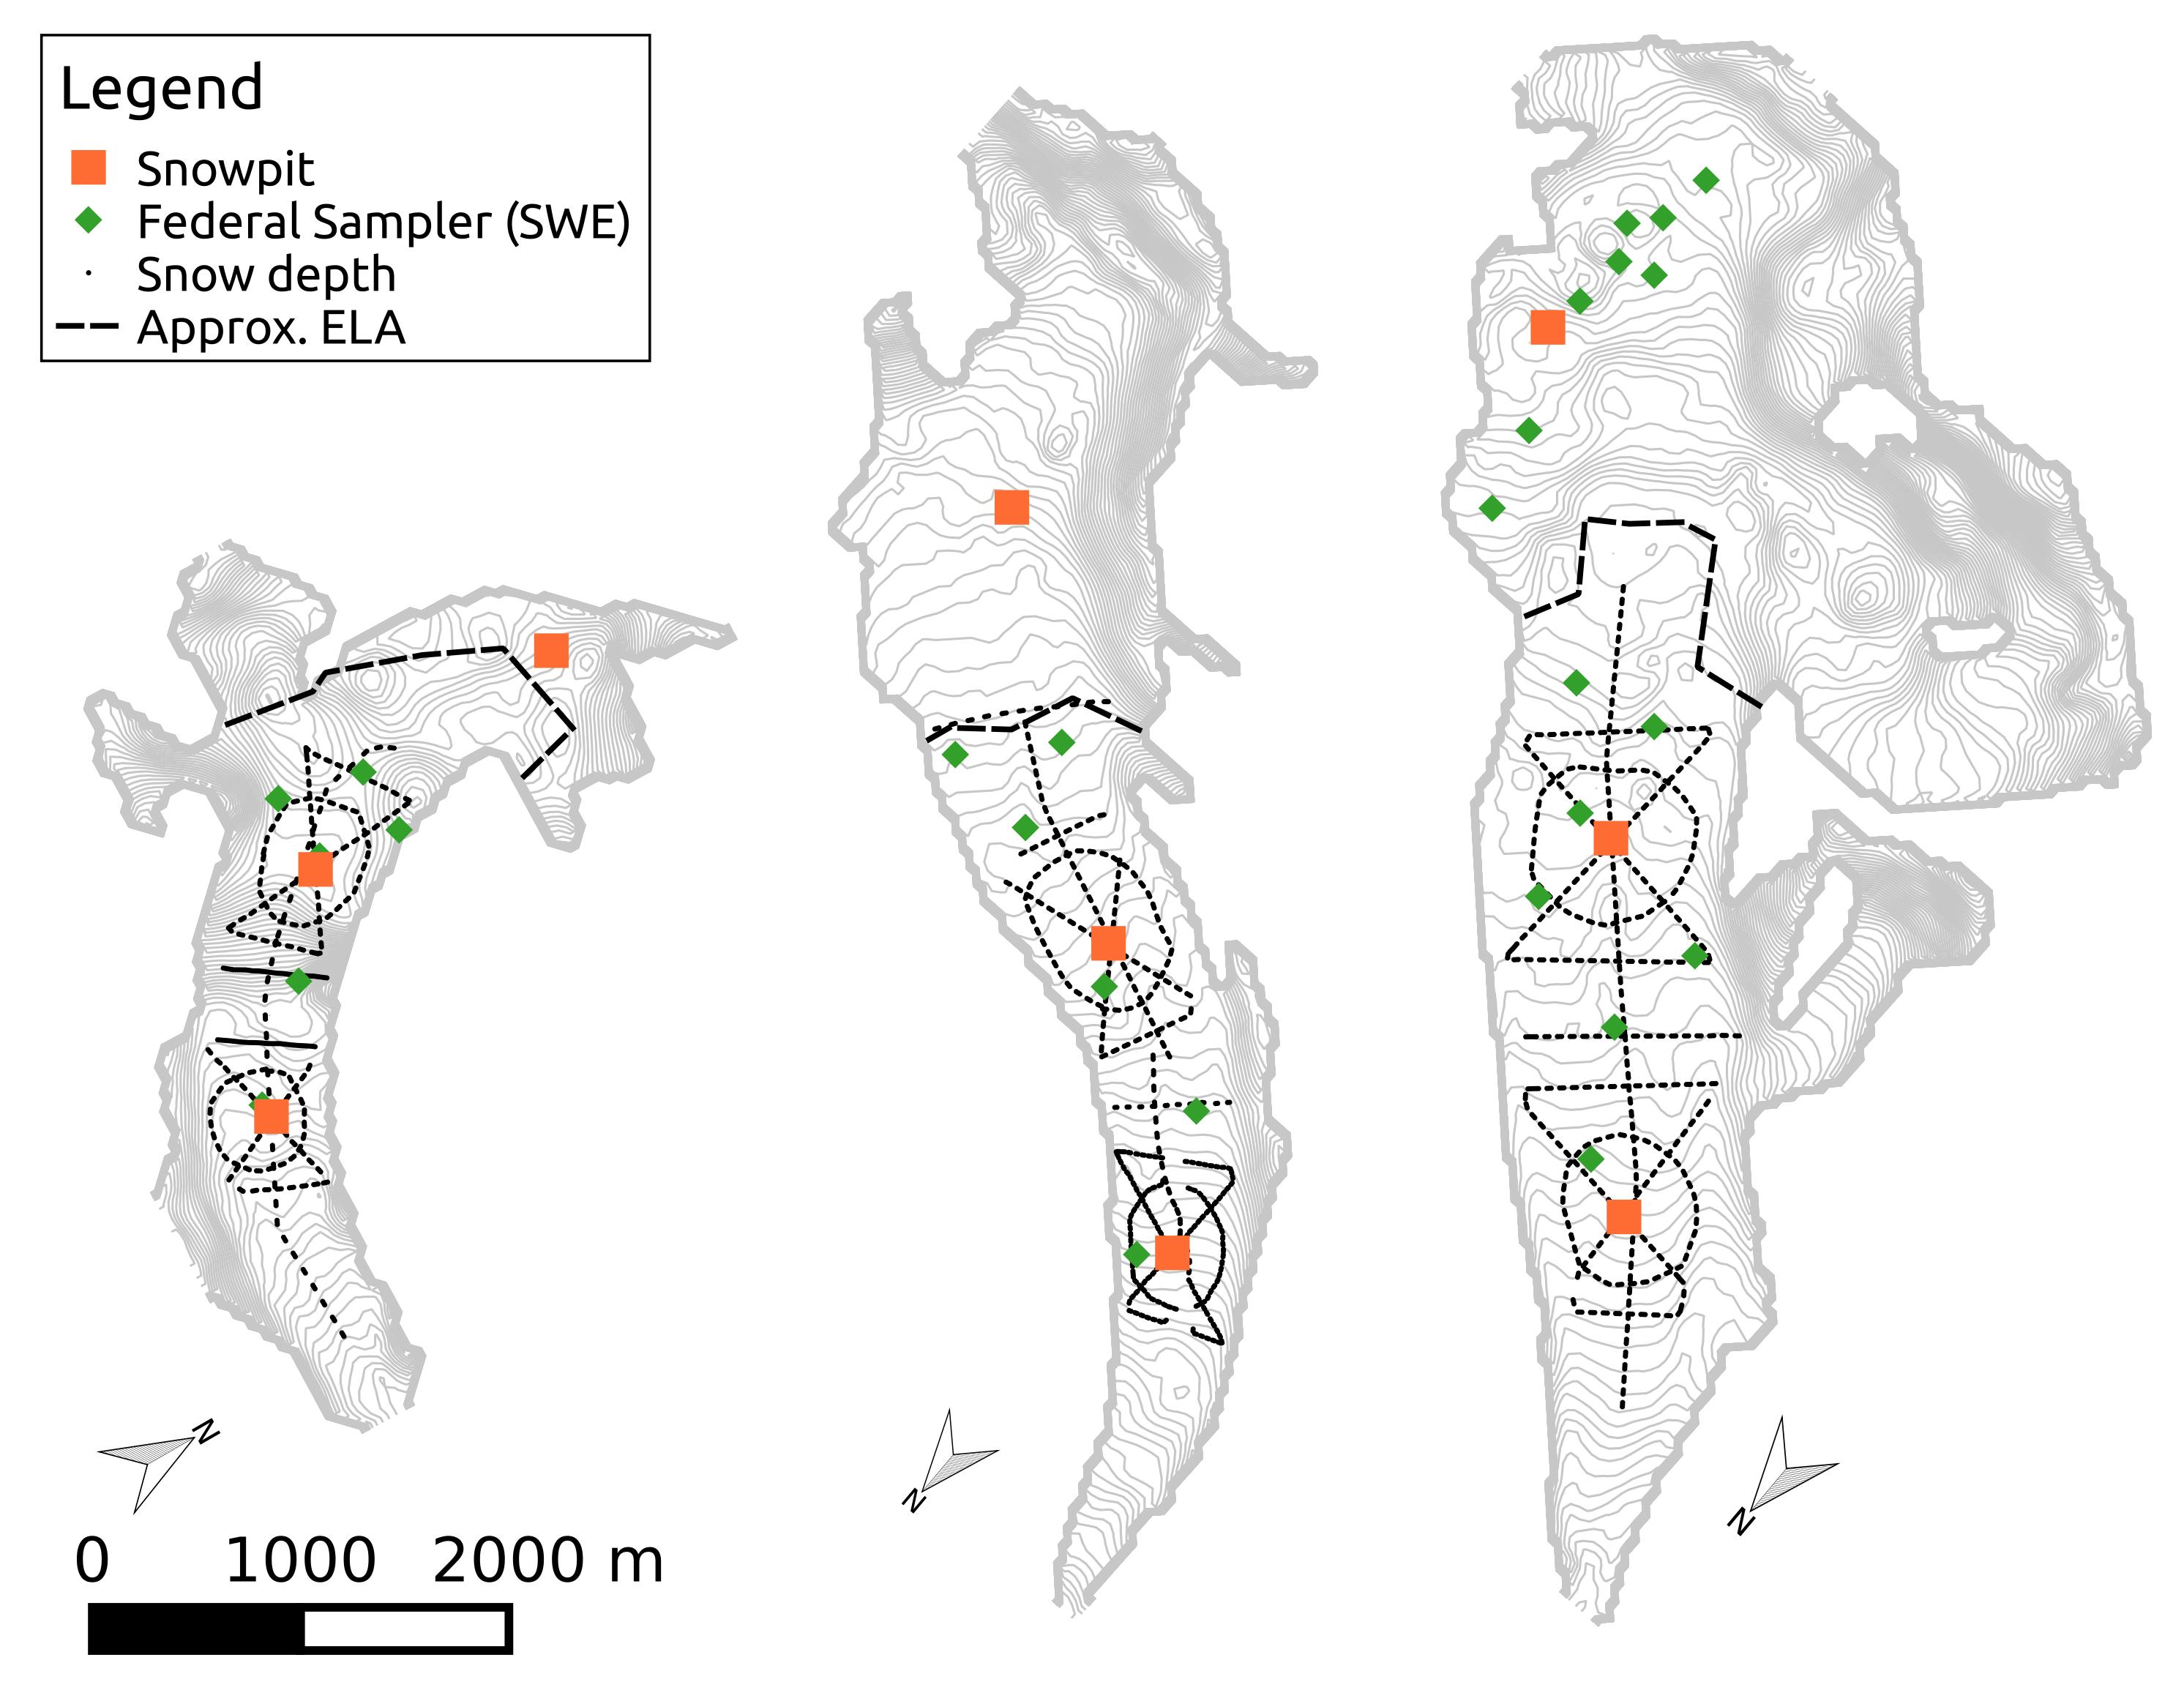
\includegraphics[height = 0.95\textwidth]{Transects_completed.jpeg}}\\
	\caption{Measurement locations for snow depth, snow pits, and SWE on three study glaciers.}
	\label{transect_completed}
\end{figure}

\begin{figure}
	\centering
	\fbox{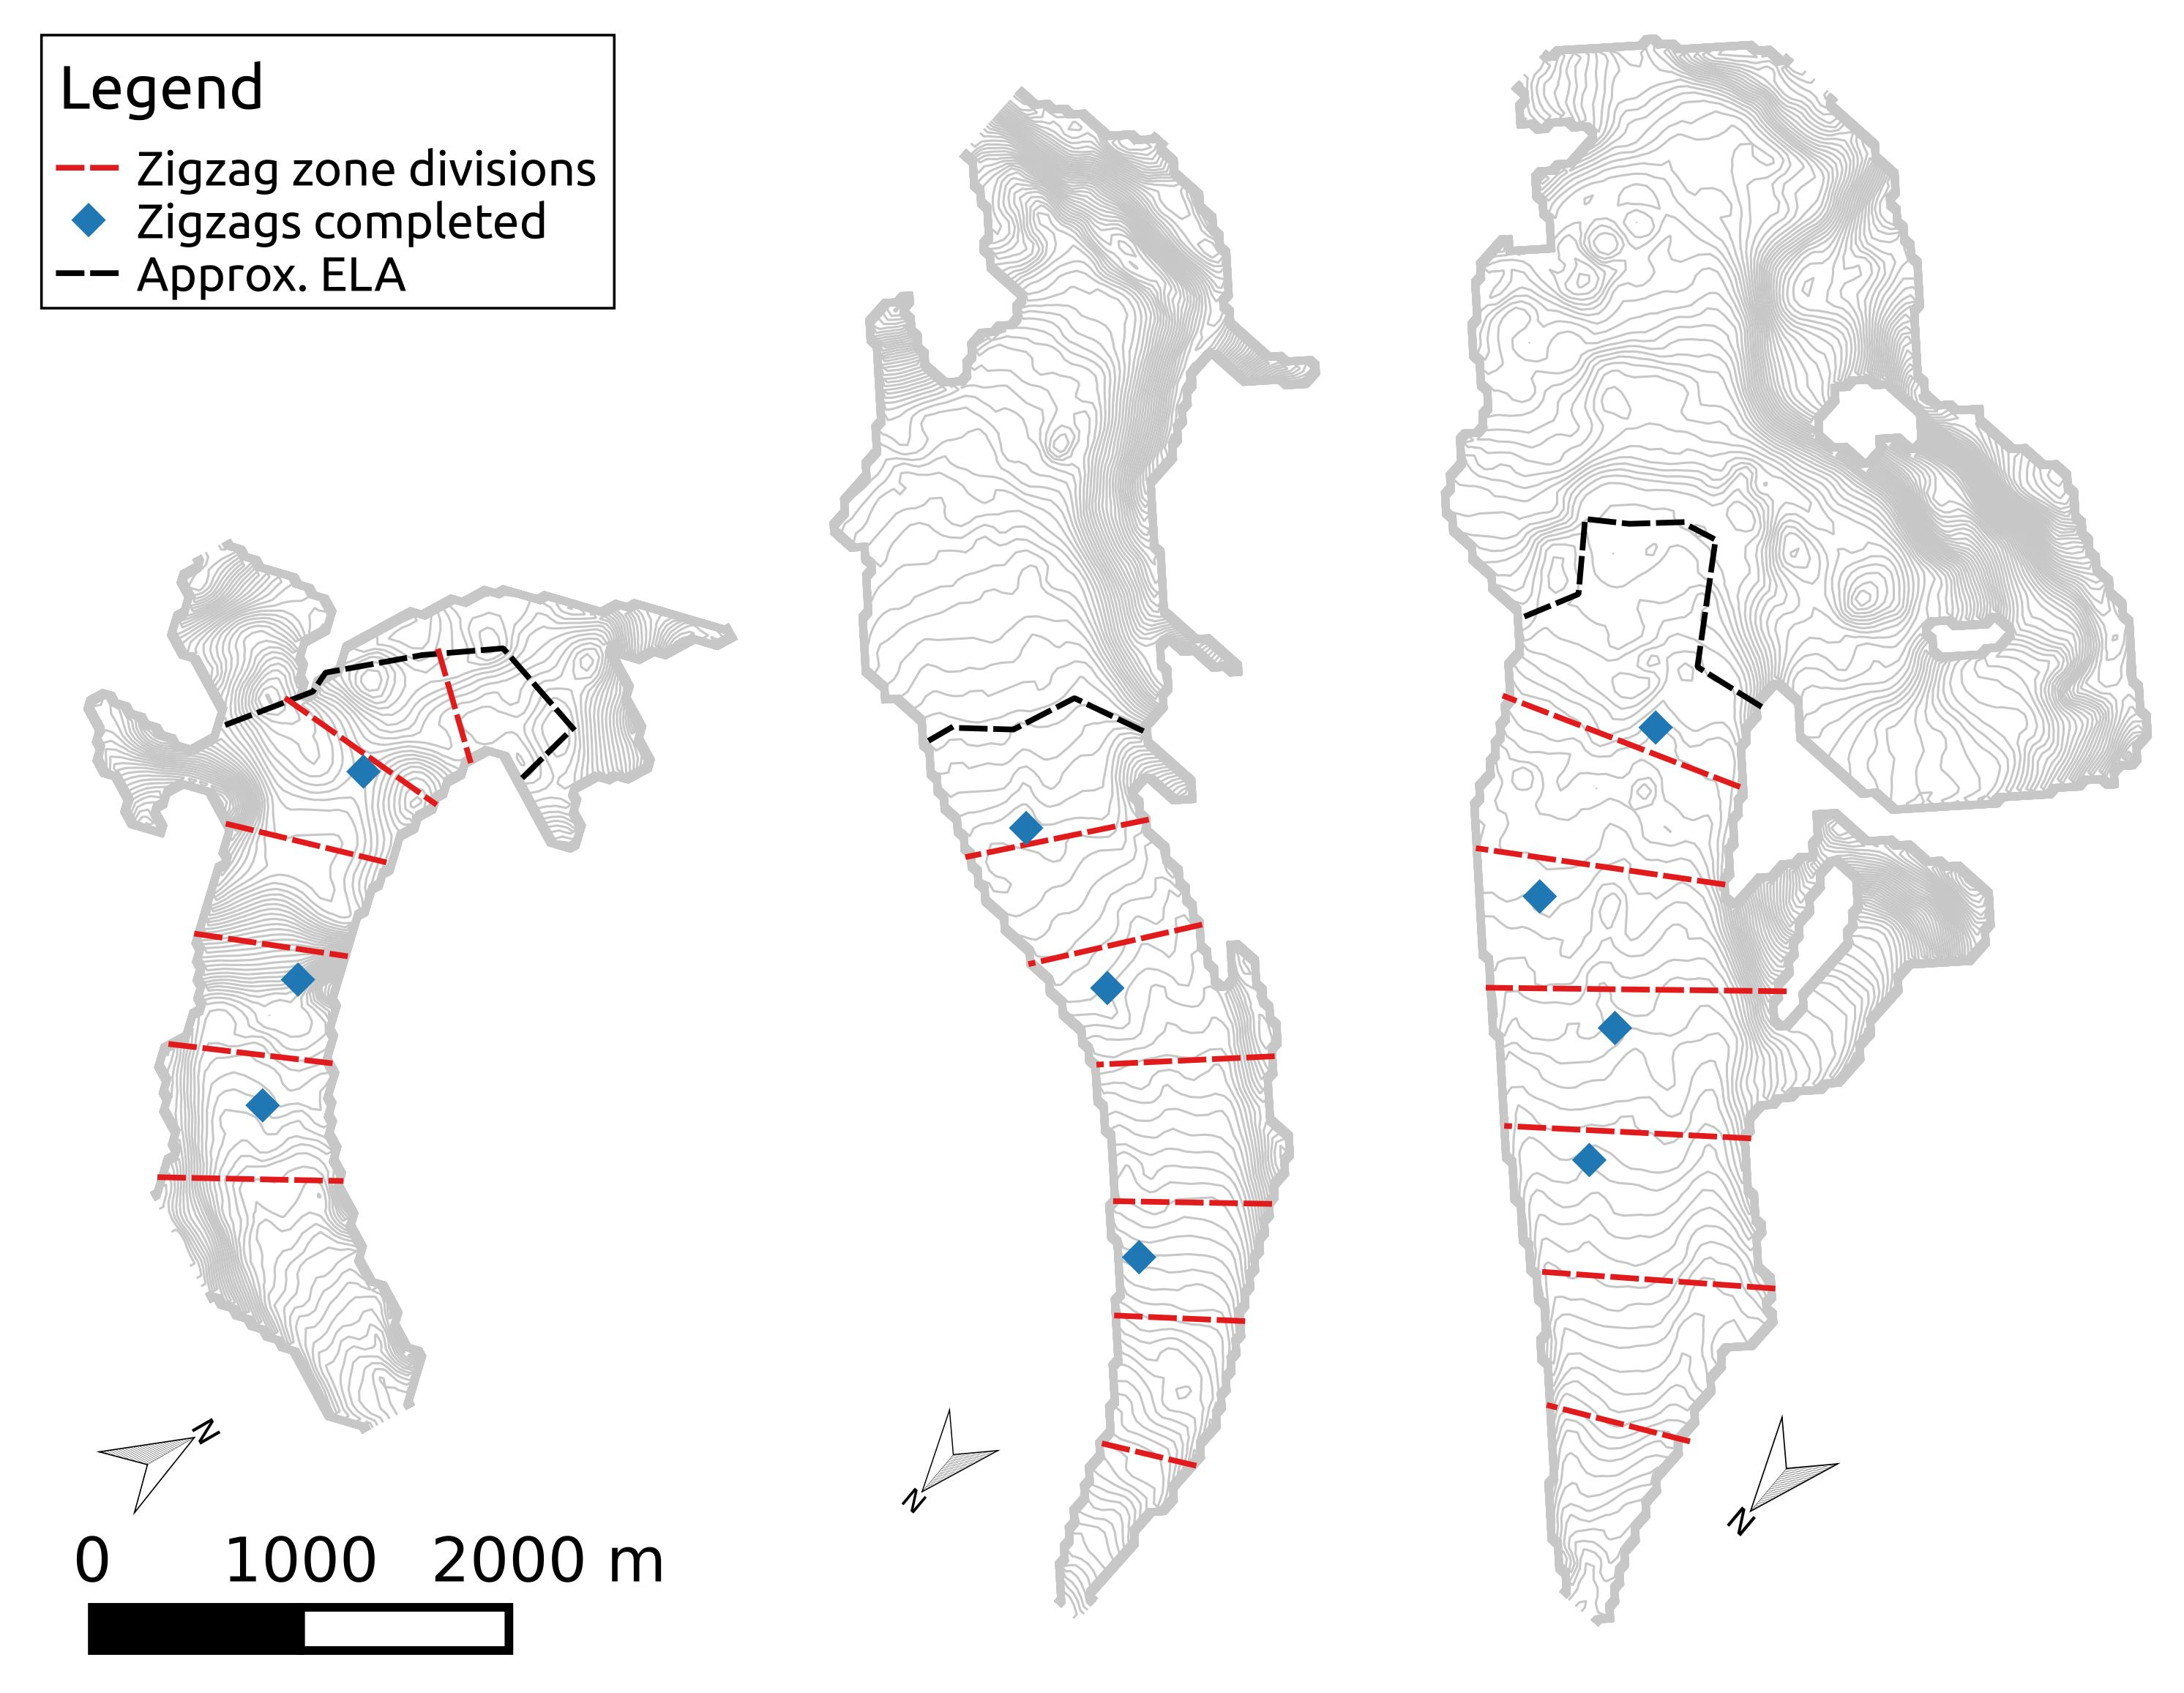
\includegraphics[height = 0.95\textwidth]{Zigzag_completed.jpeg}}\\
	\caption{Locations of completed zigzag measurements in the ablation area (divided into seven zones).}
	\label{zigzag_completed}
\end{figure}
\end{landscape}


\subsection{To Do}
\begin{itemize}
\item Sew megamid snow skirt
\item Figure out tare weight issue of SWE tube
\item Figure out why vertex naming was out of order on GPS device
\item Figure out stove situation because the whisper lite stoves were flaring and fuel was leaking
\end{itemize} 

\subsection{Next time}
\begin{itemize}
\item Dedicated thermos for starter water
\item Dedicated snow scooper
\item Get an InReach? The one borrowed from KLRS worked really well
\item More dowels for megamid?
\item Bring dull, plastic shovel for digging out megamid
\item Have dedicated snow board to determine accumulation during trip
\end{itemize}

\subsection{Thoughts on Data}

\begin{itemize}
\item Snow depth sources of error: depth probes lost tips, surface micro topography (especially in areas where melt had begun), probe not being vertical
\item Was there a systematic difference between depths measured by different observers?
\item What was the GPS device uncertainty and how will that be incorporated?
\item DEM was not reliable for areas in Glacier 4. How accurate is it? How would elevation errors affect topographic parameters calculated from the DEM?
\item How do SWE values from the Federal Sampler and snow pit compare?
\item How do we estimate SWE values at each depth measurement location (e.g. average of all density values, divided into area, weighted mean)? And how does this affect balance values and errors in SWE estimation? 
\item Is the data sensitive to distance between observers (9.5--11m)?
\end{itemize}

\bibliography{/home/glaciology1/Documents/MastersDocuments/MastersLit}
\bibliographystyle{igs}

\pagebreak
\section*{Appendix I - Field maps}

\noindent \large{\textbf{Glacier 4}}\\
\fbox{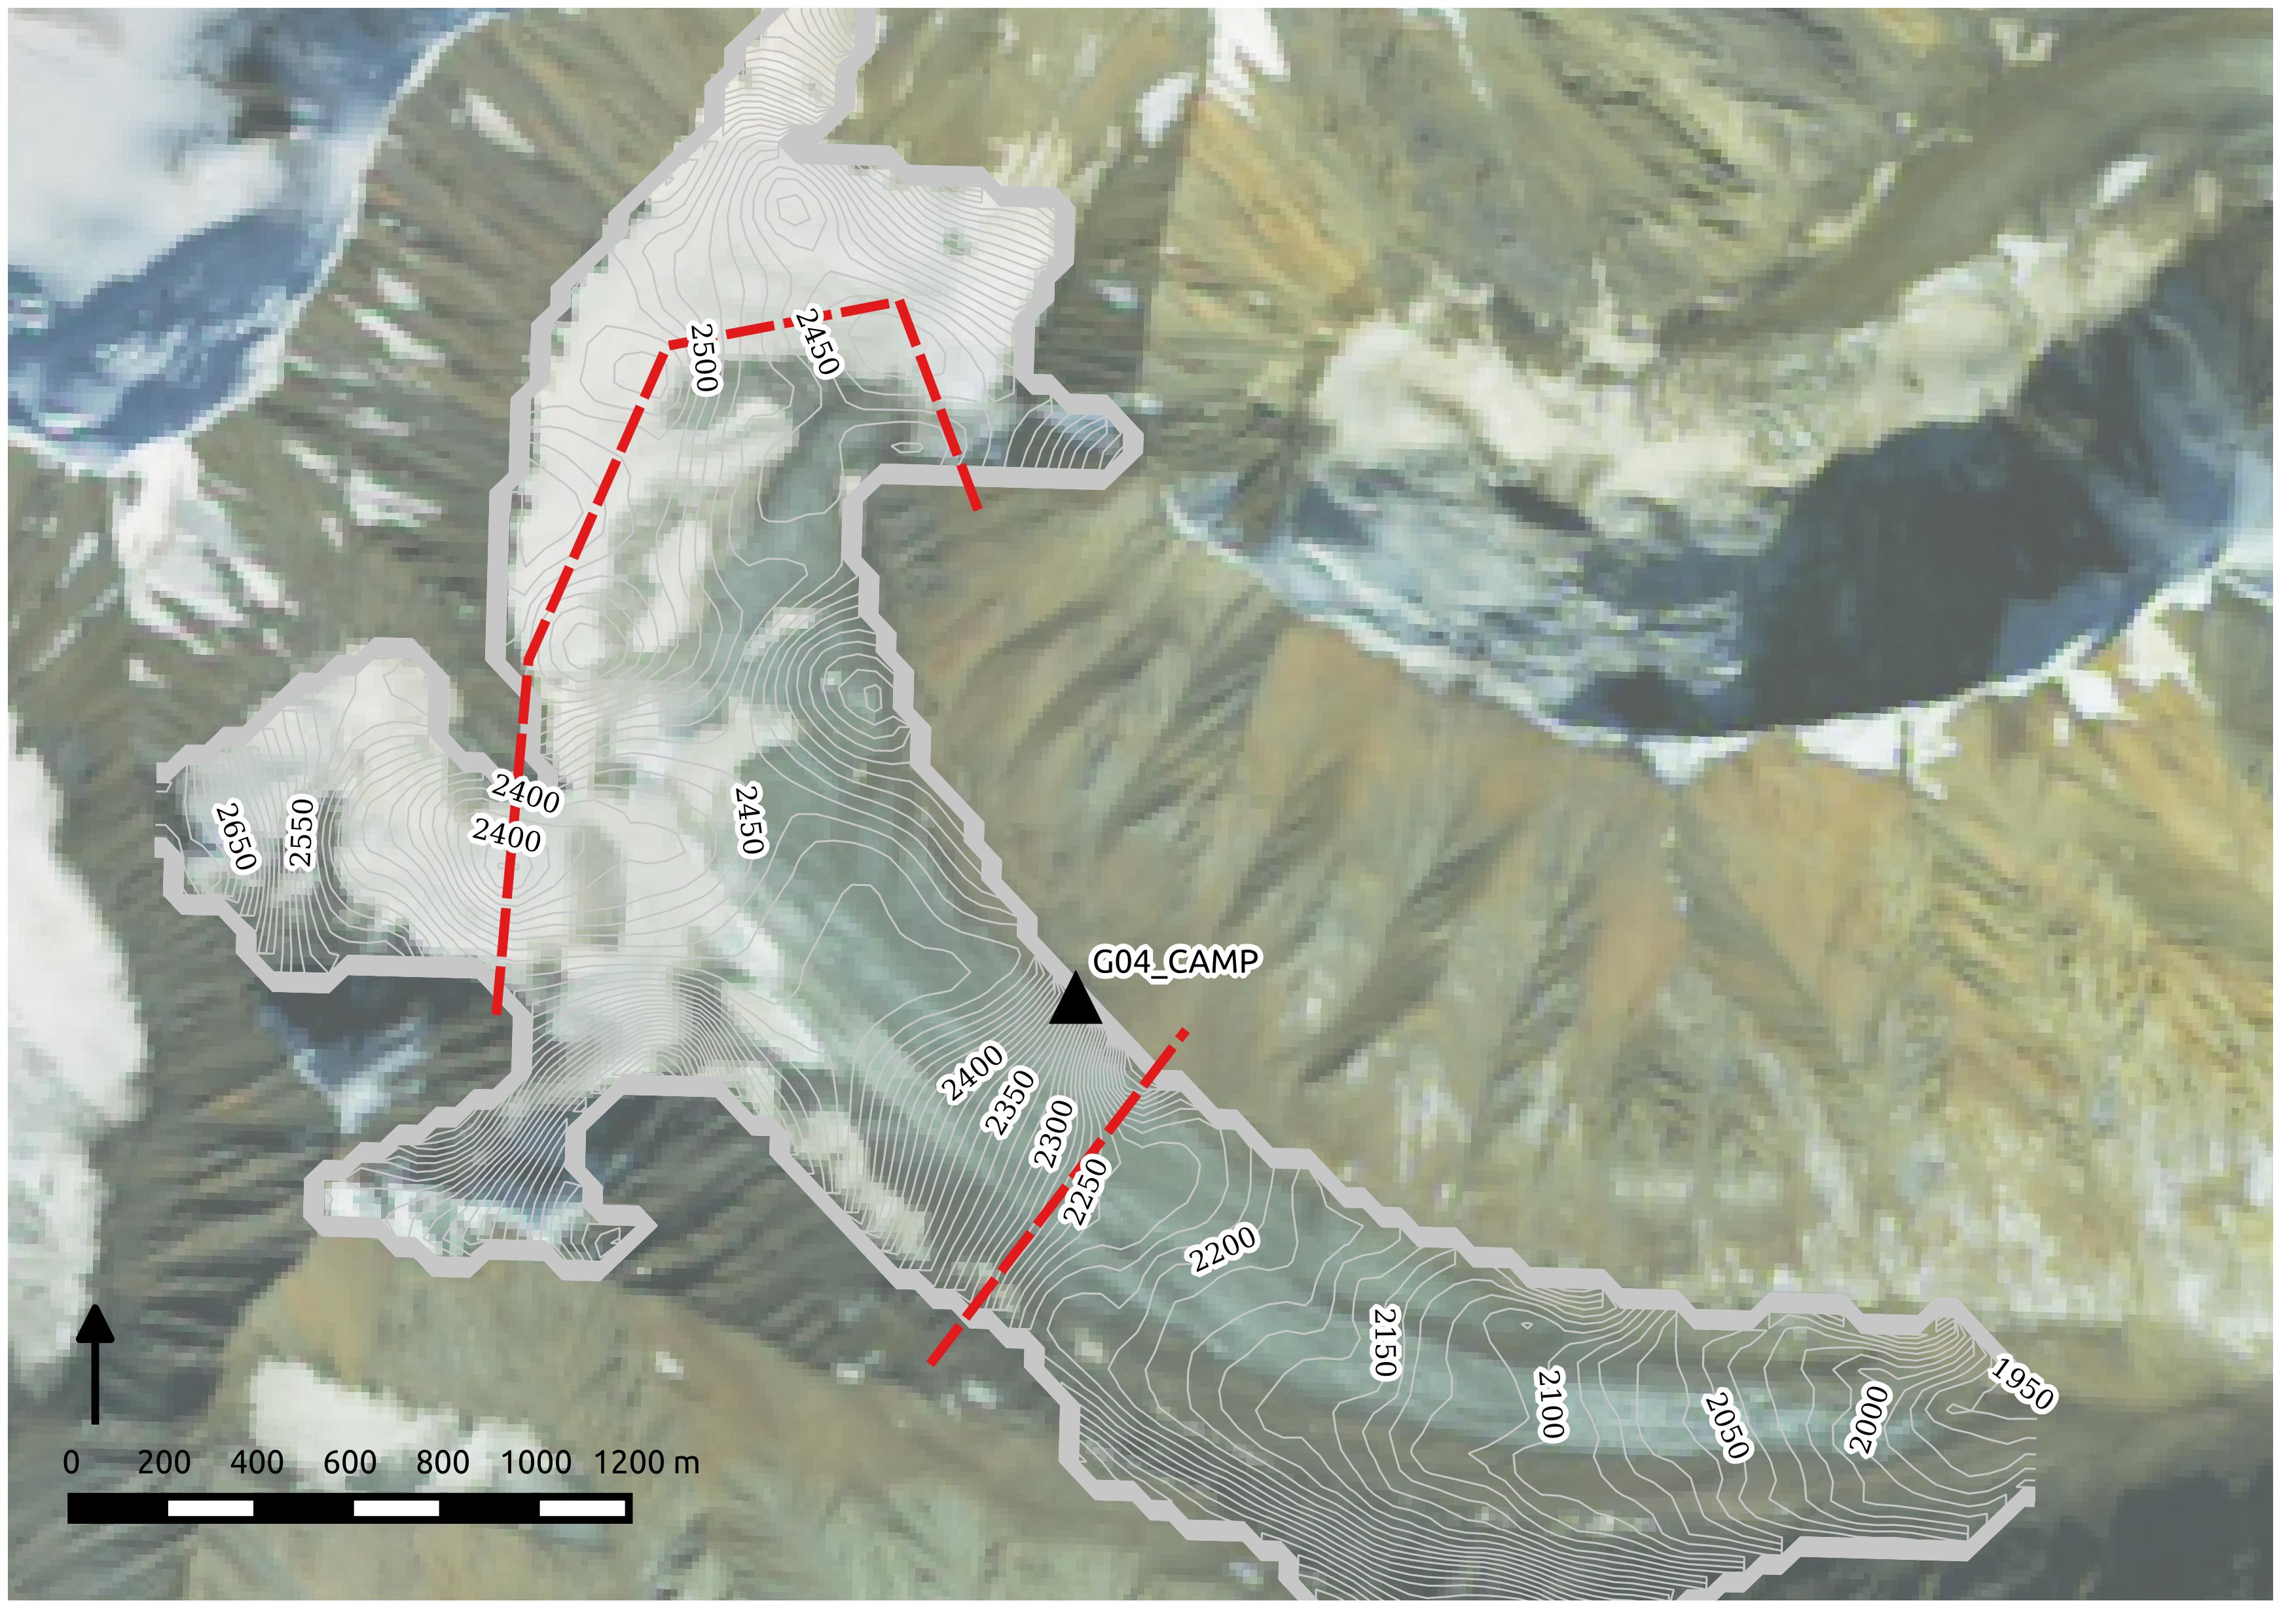
\includegraphics[height = 0.45\textheight]{G04_Topo.jpeg}}\\
\fbox{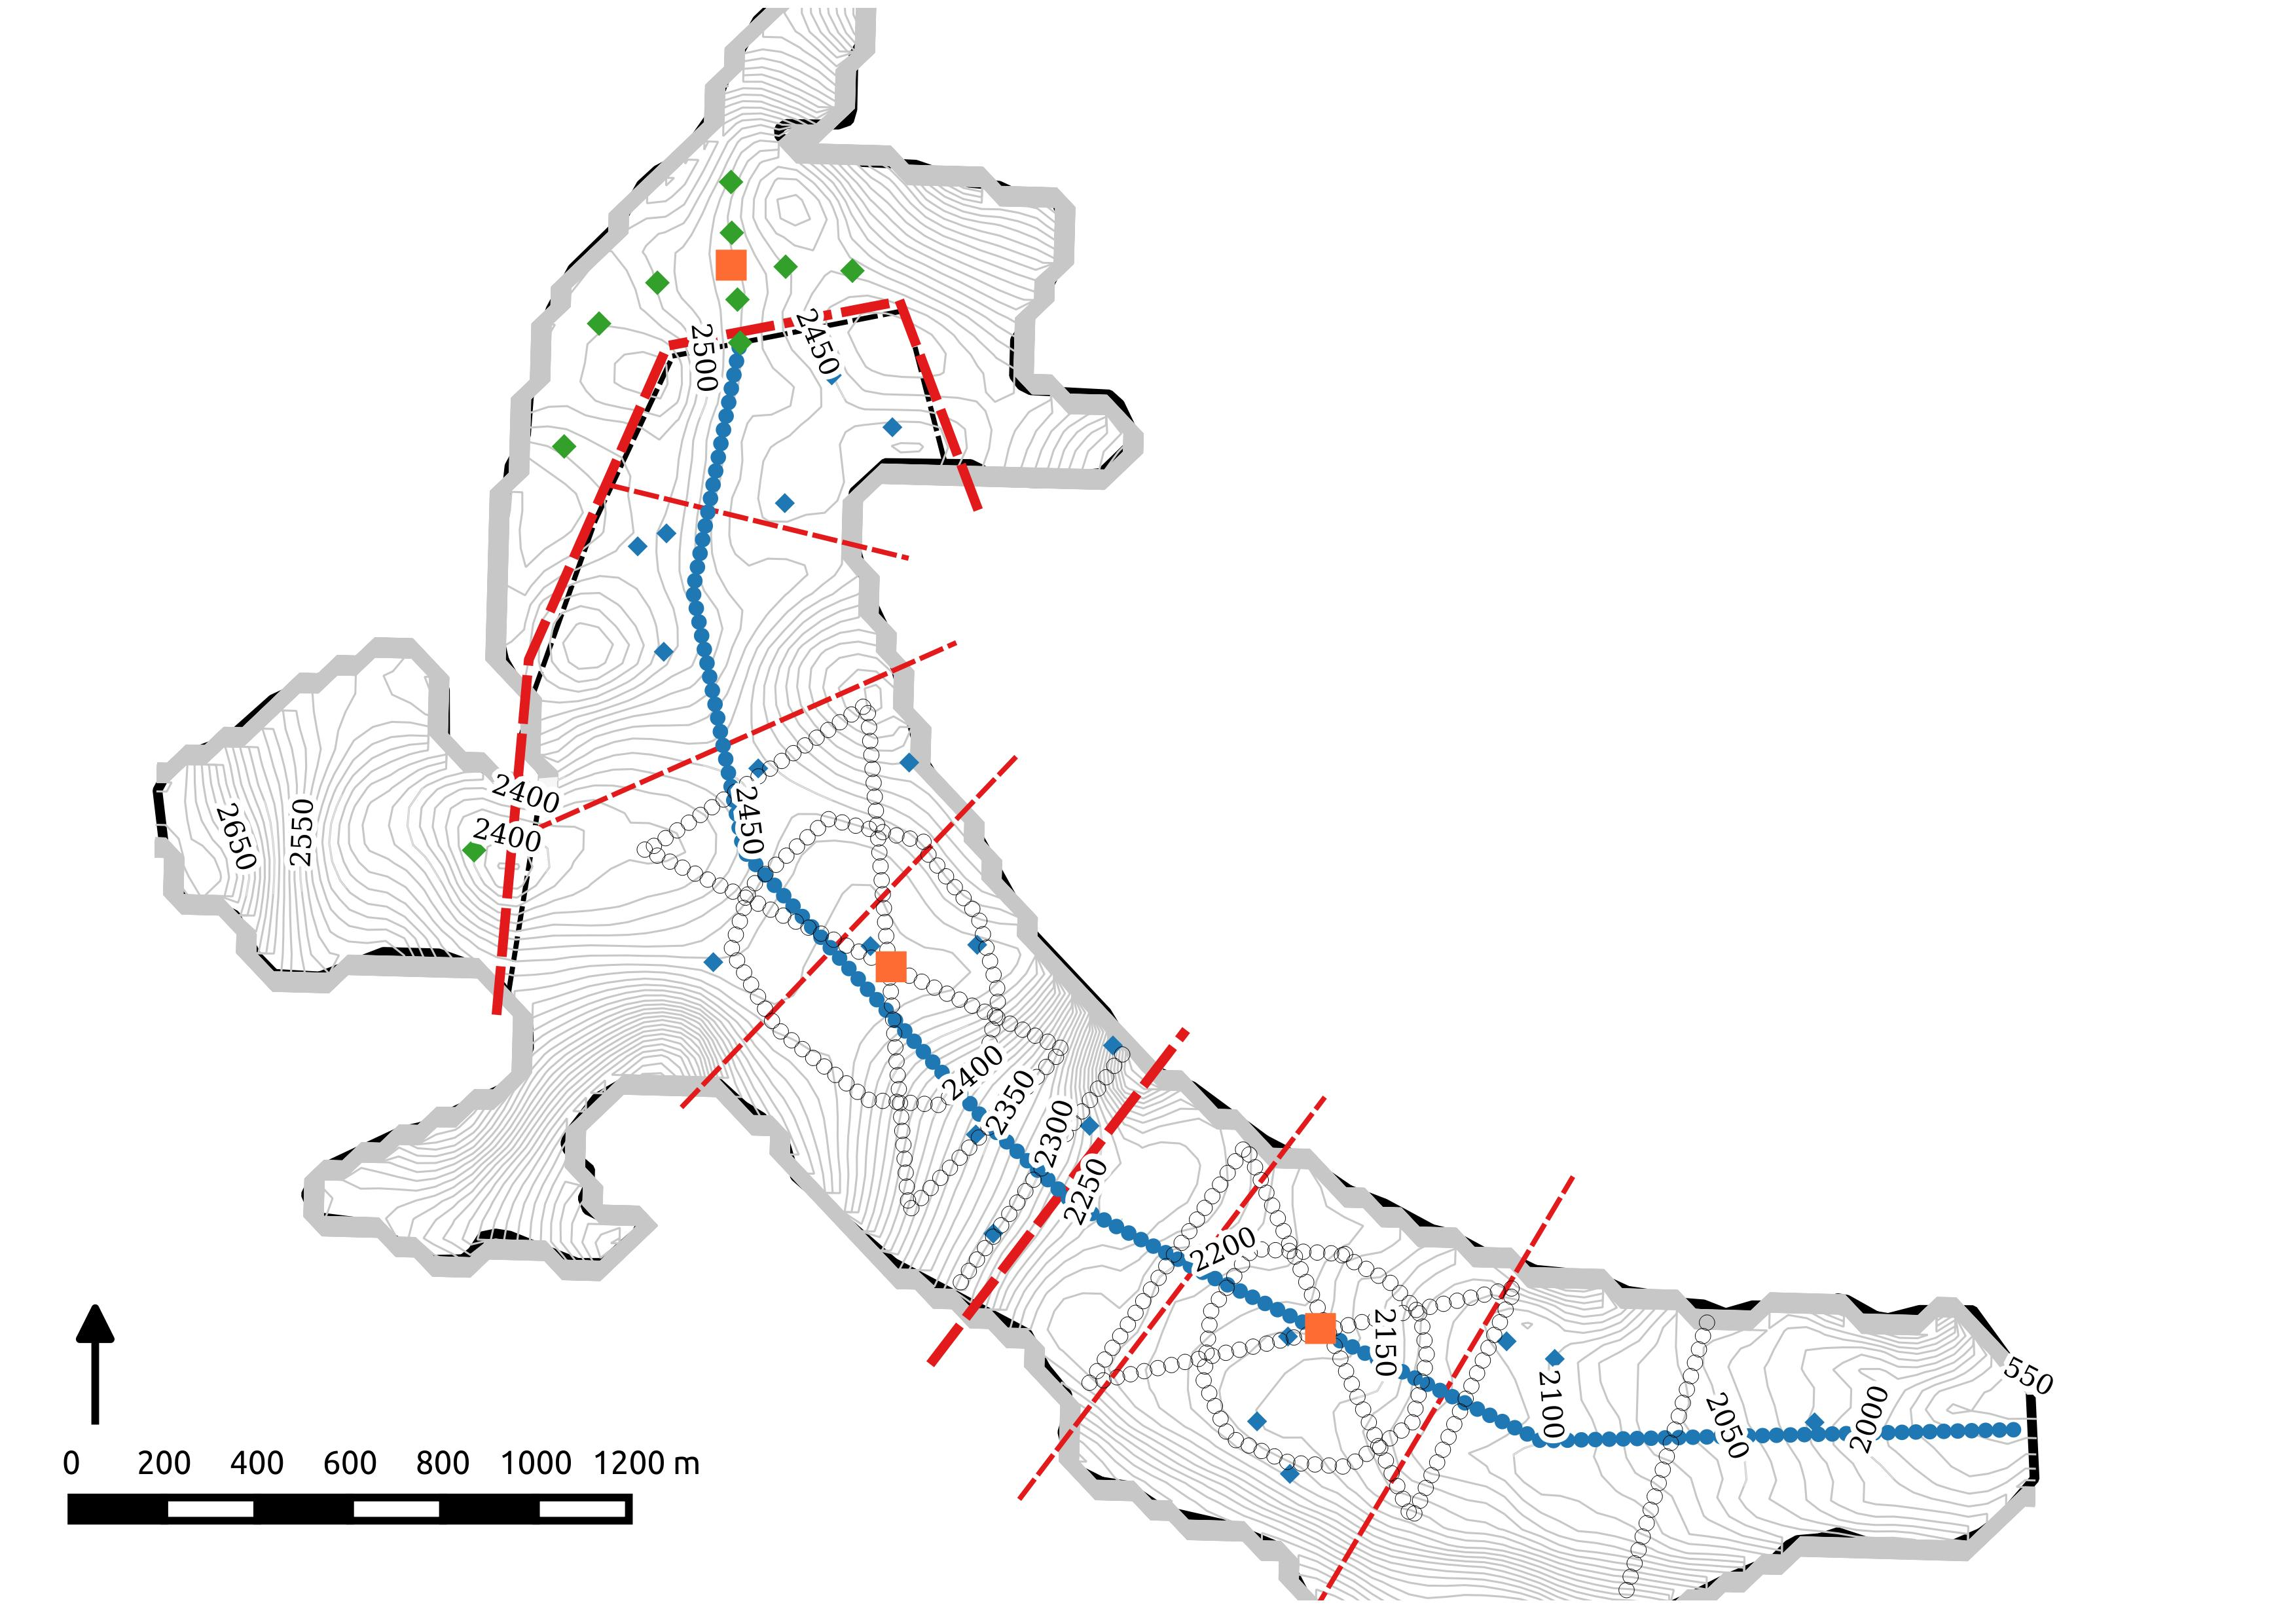
\includegraphics[height = 0.45\textheight]{G04_Overview.jpeg}}\\
\fbox{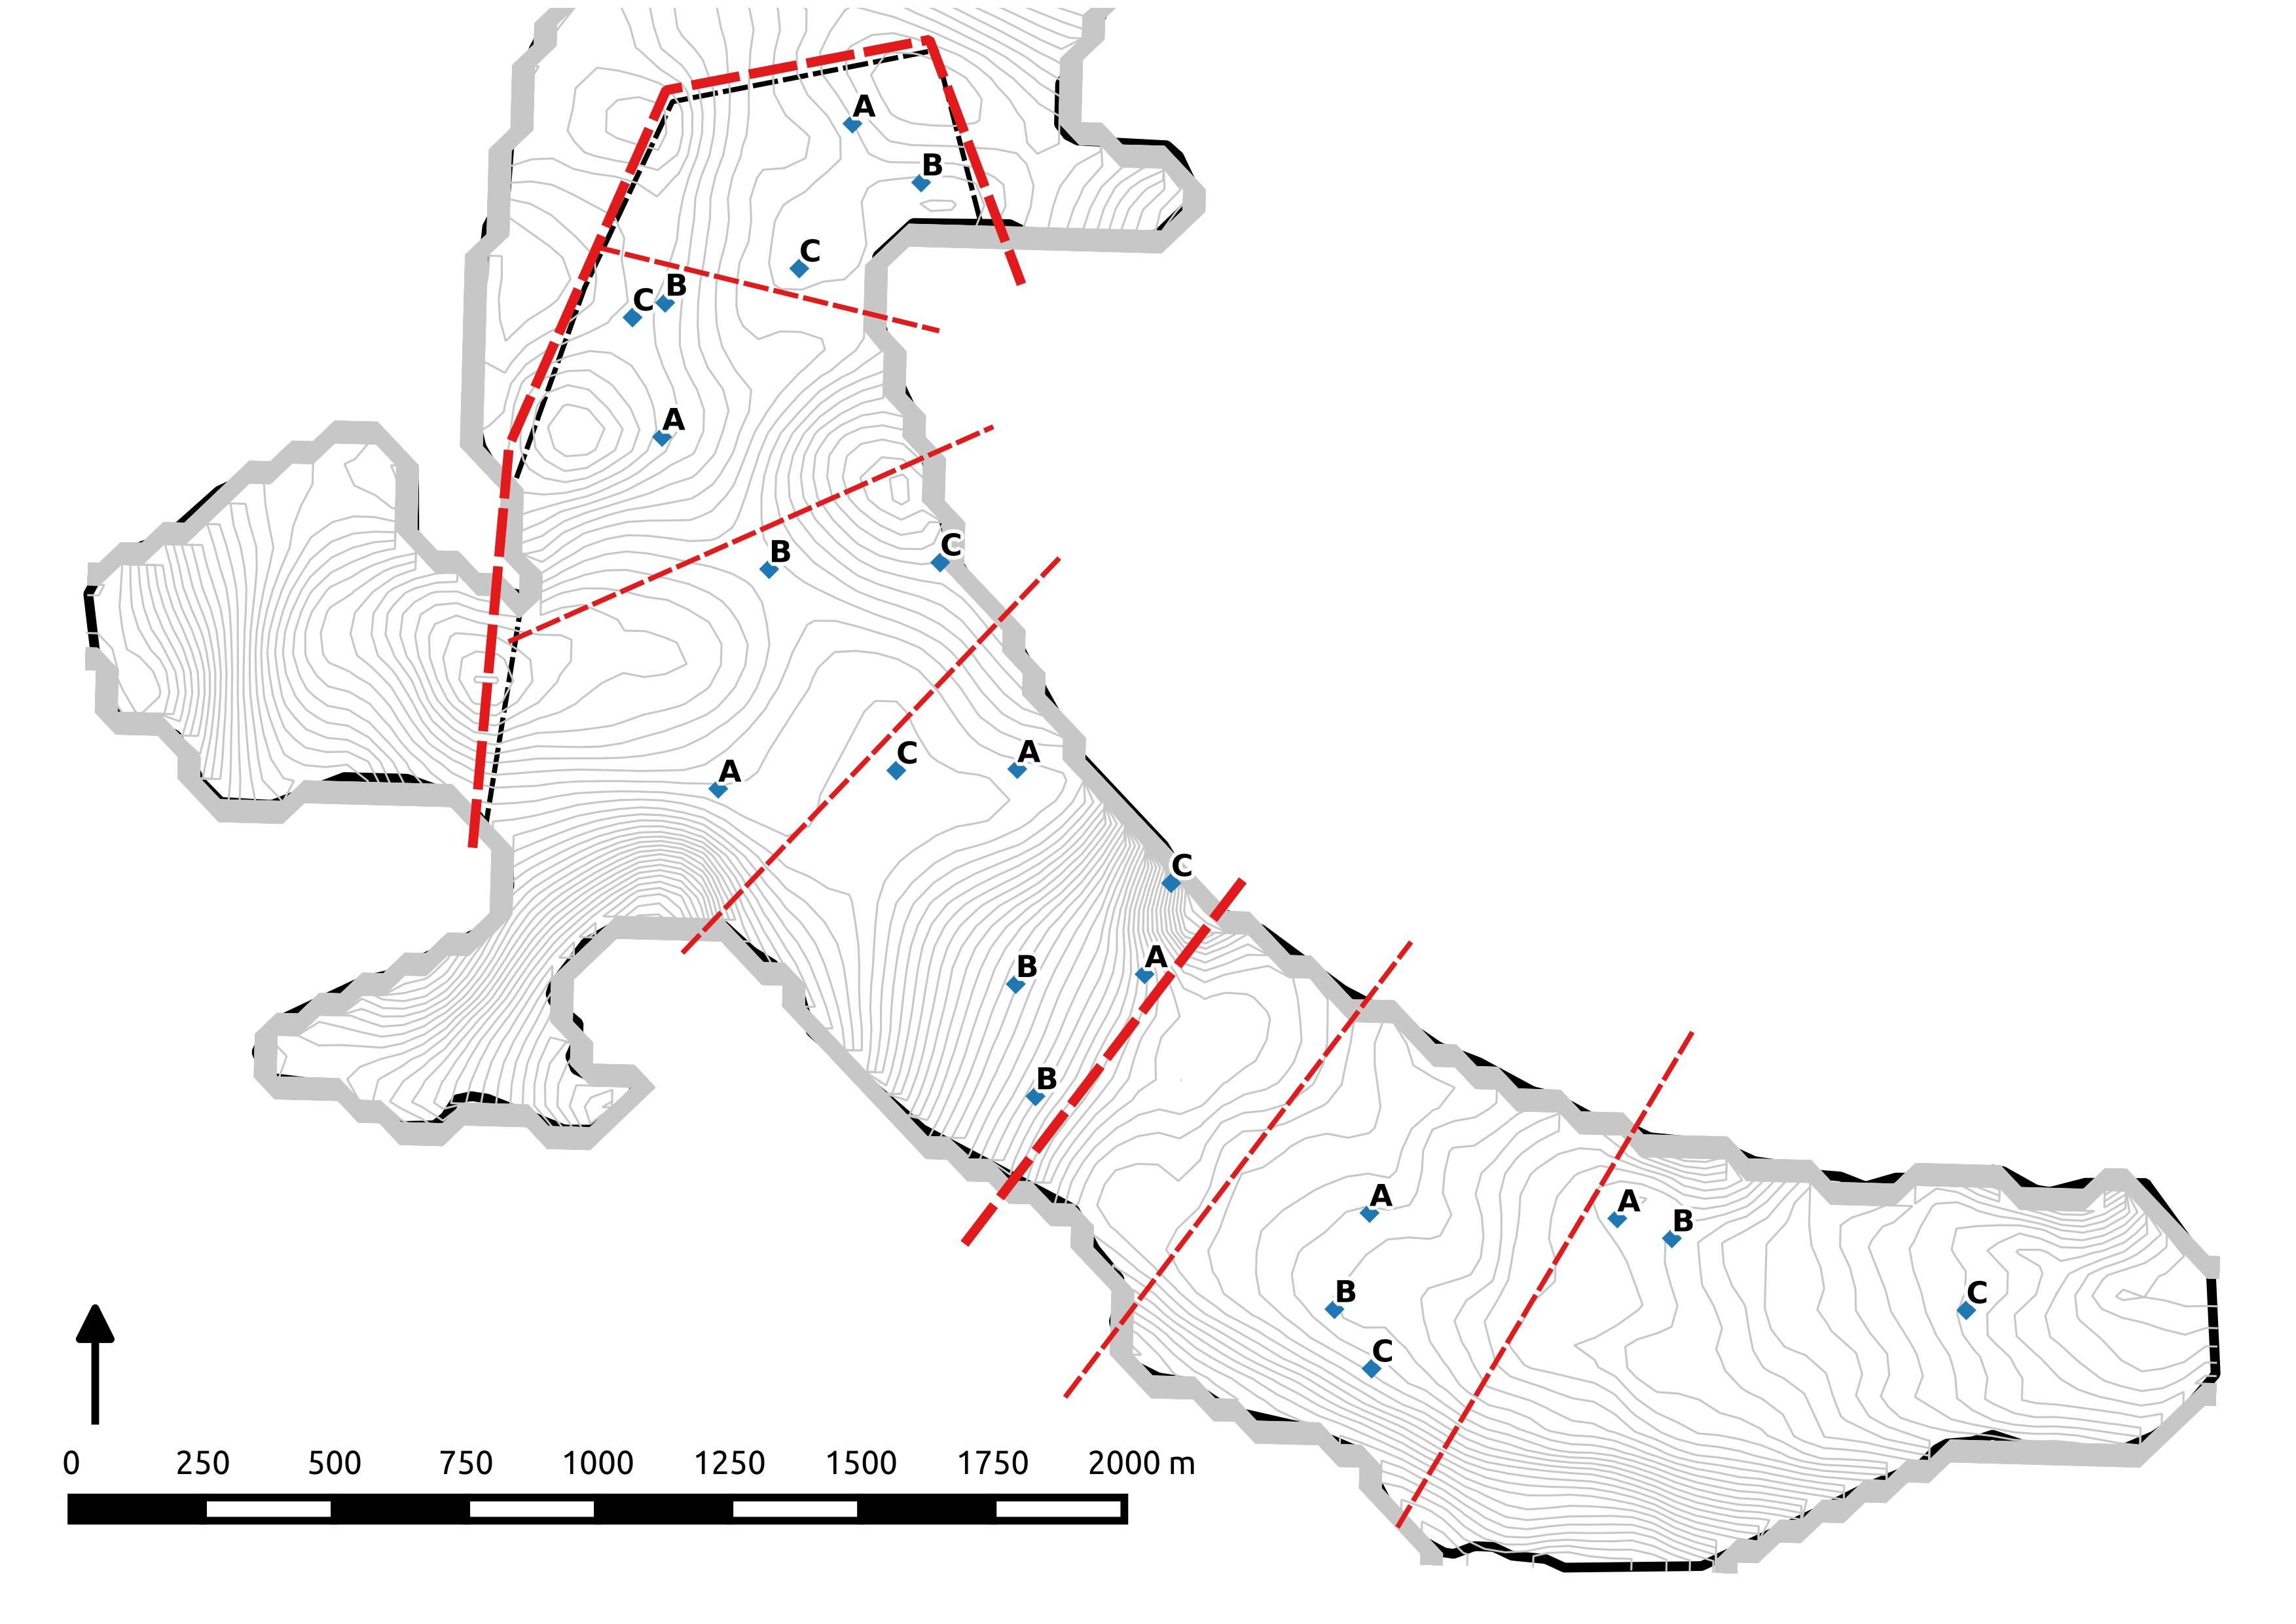
\includegraphics[height = 0.45\textheight]{G04_ZZ.jpeg}}\\
\fbox{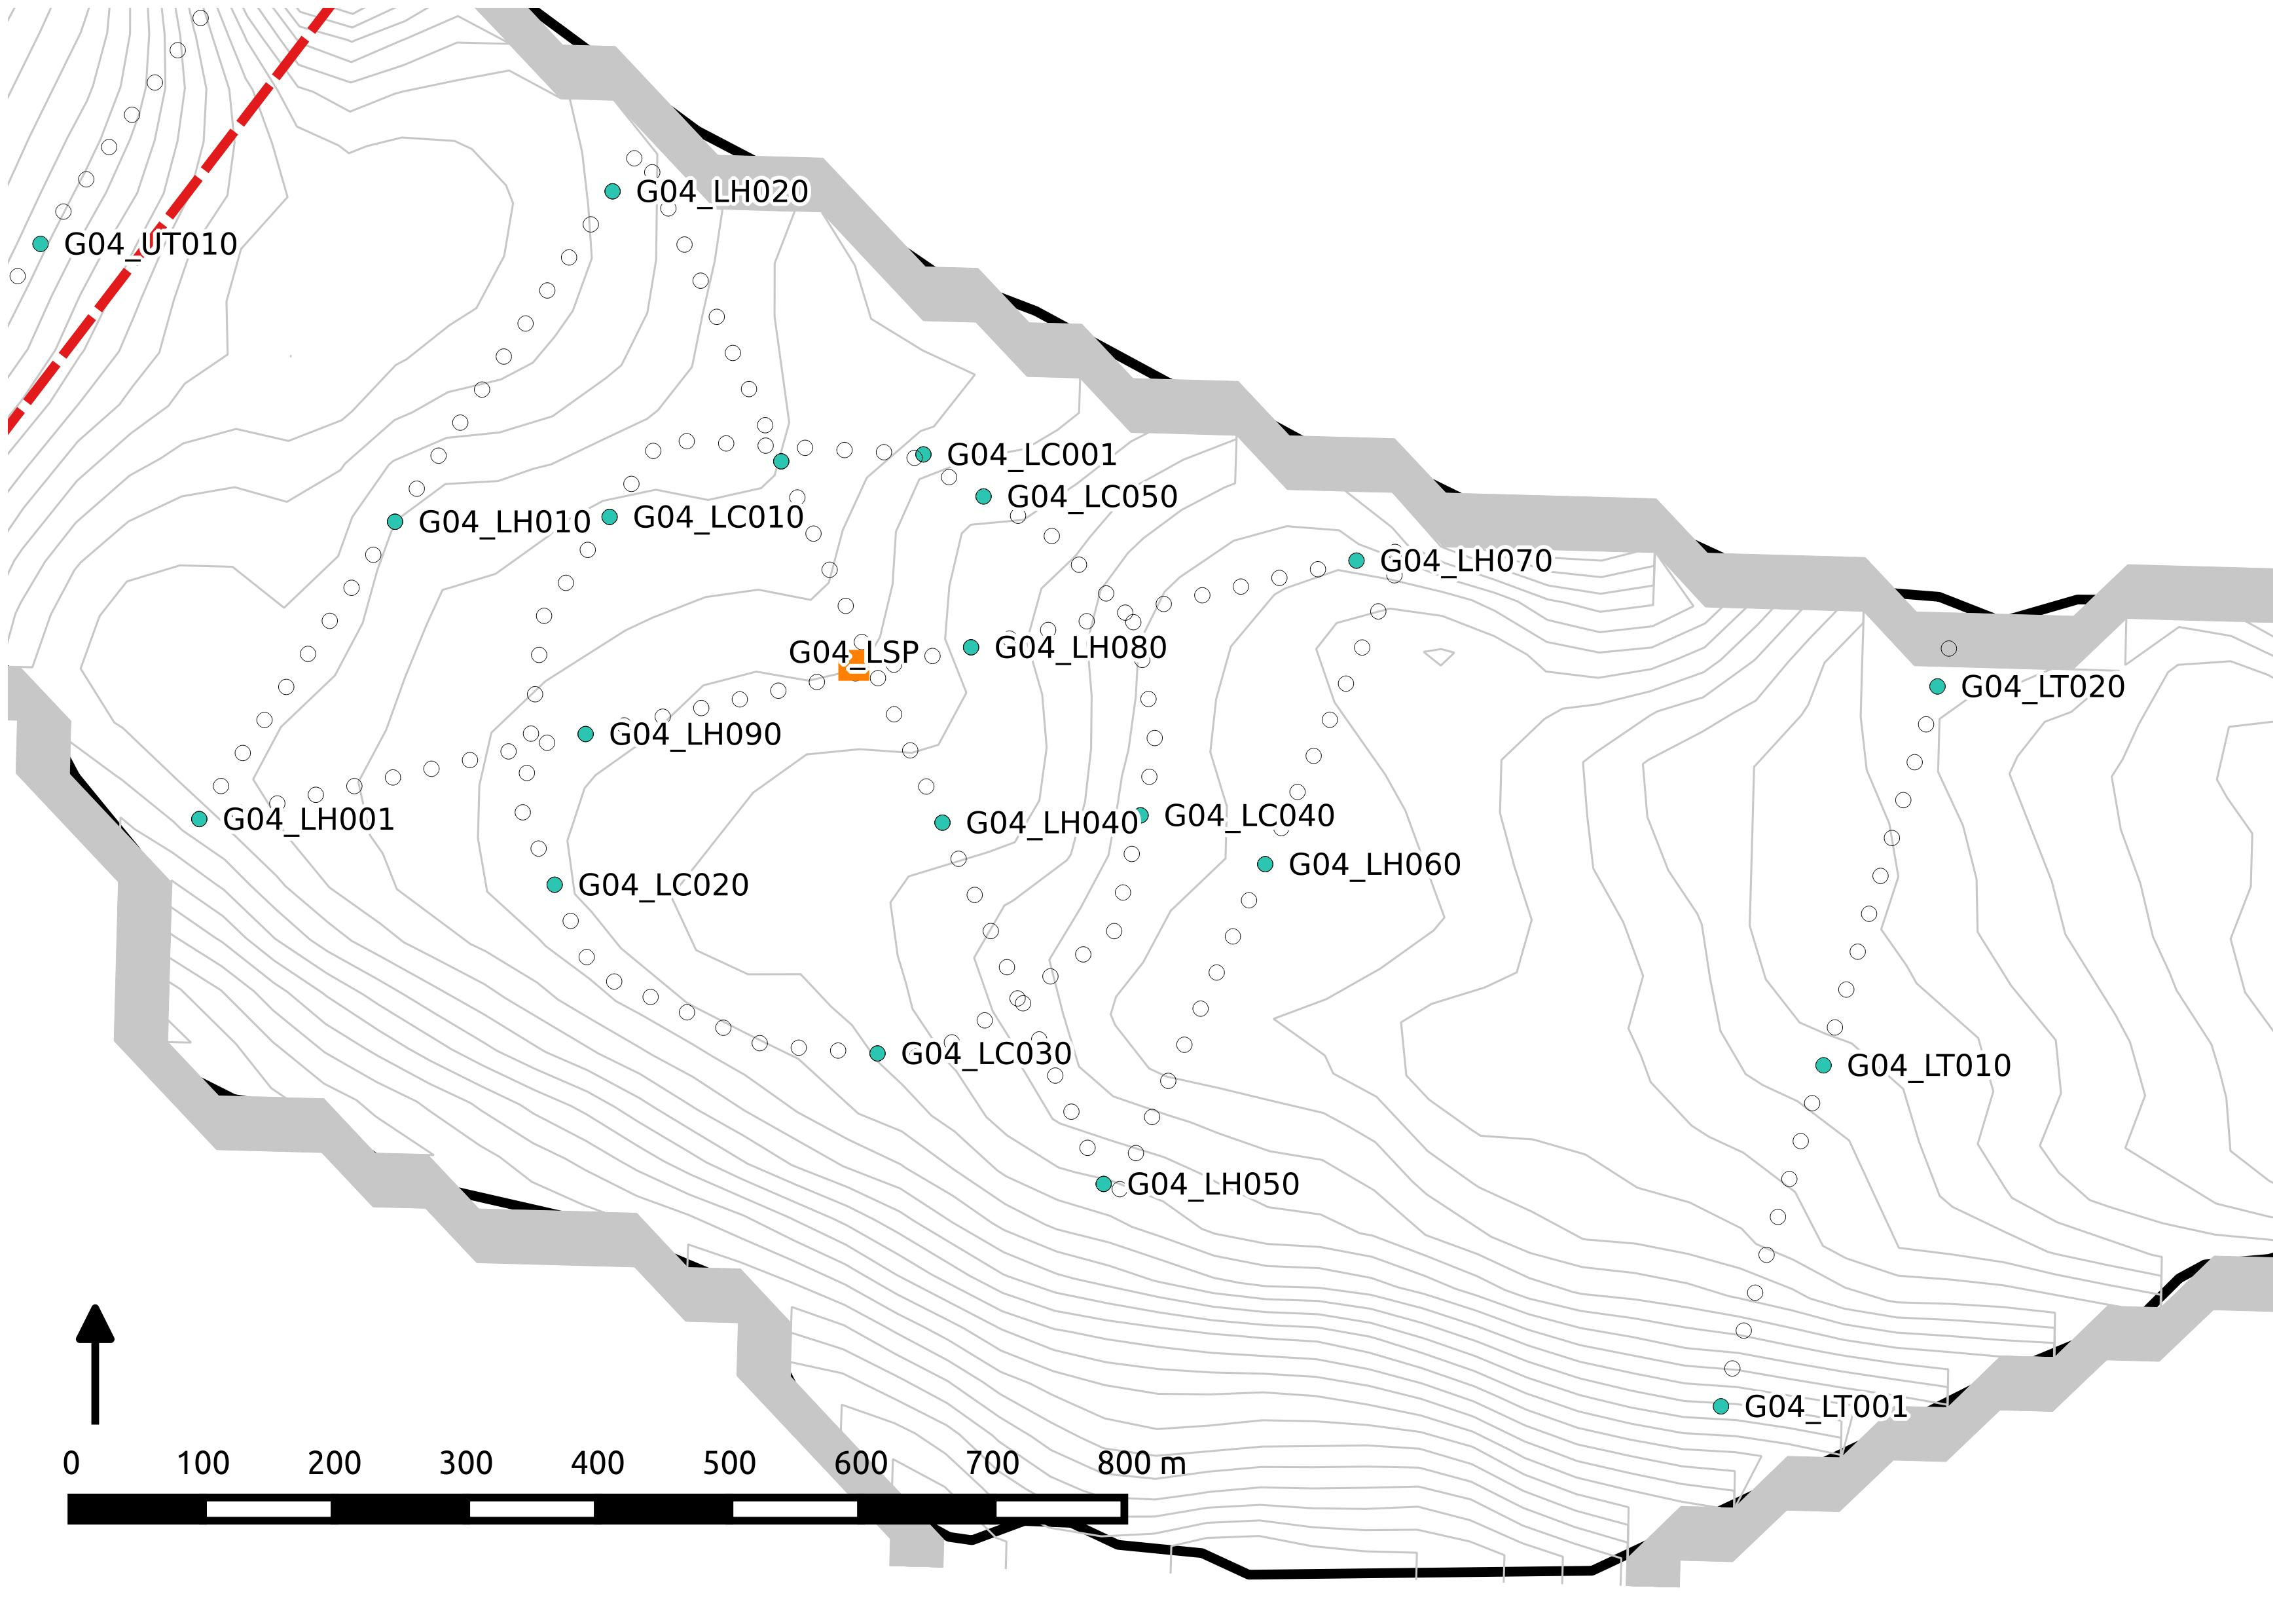
\includegraphics[height = 0.45\textheight]{G04_LH.jpeg}}\\
\fbox{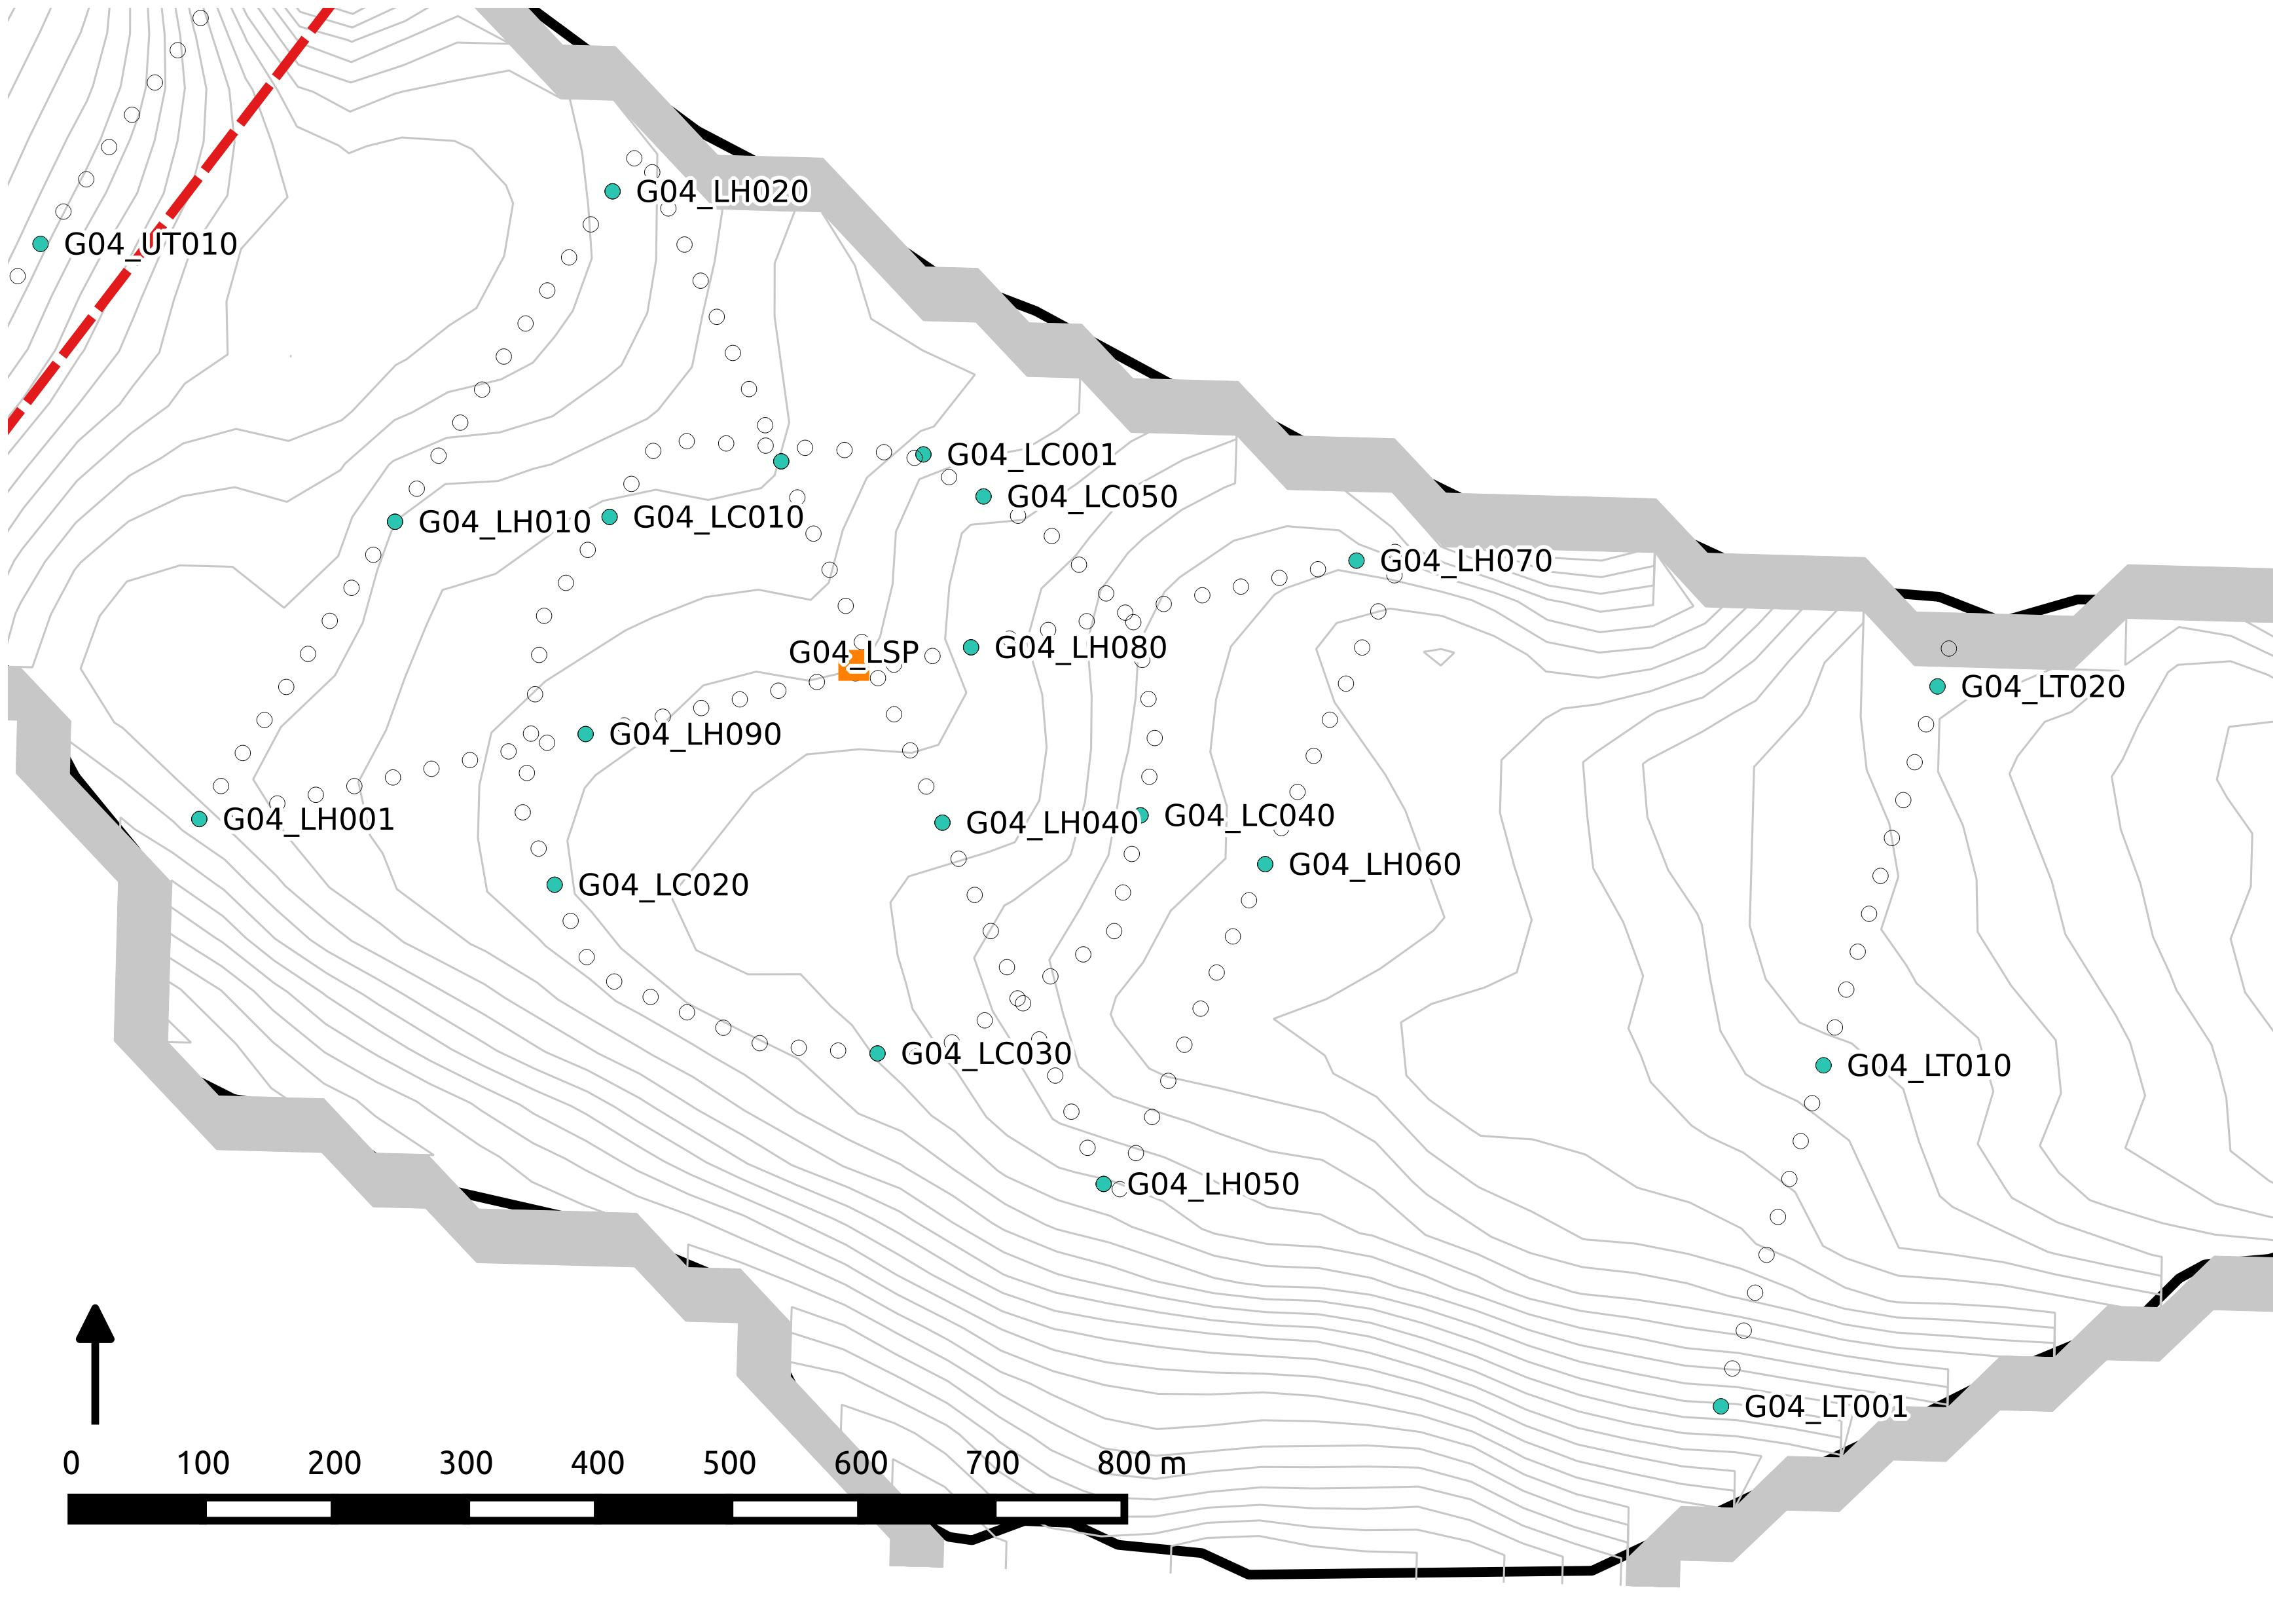
\includegraphics[height = 0.45\textheight]{G04_LH.jpeg}}\\
\fbox{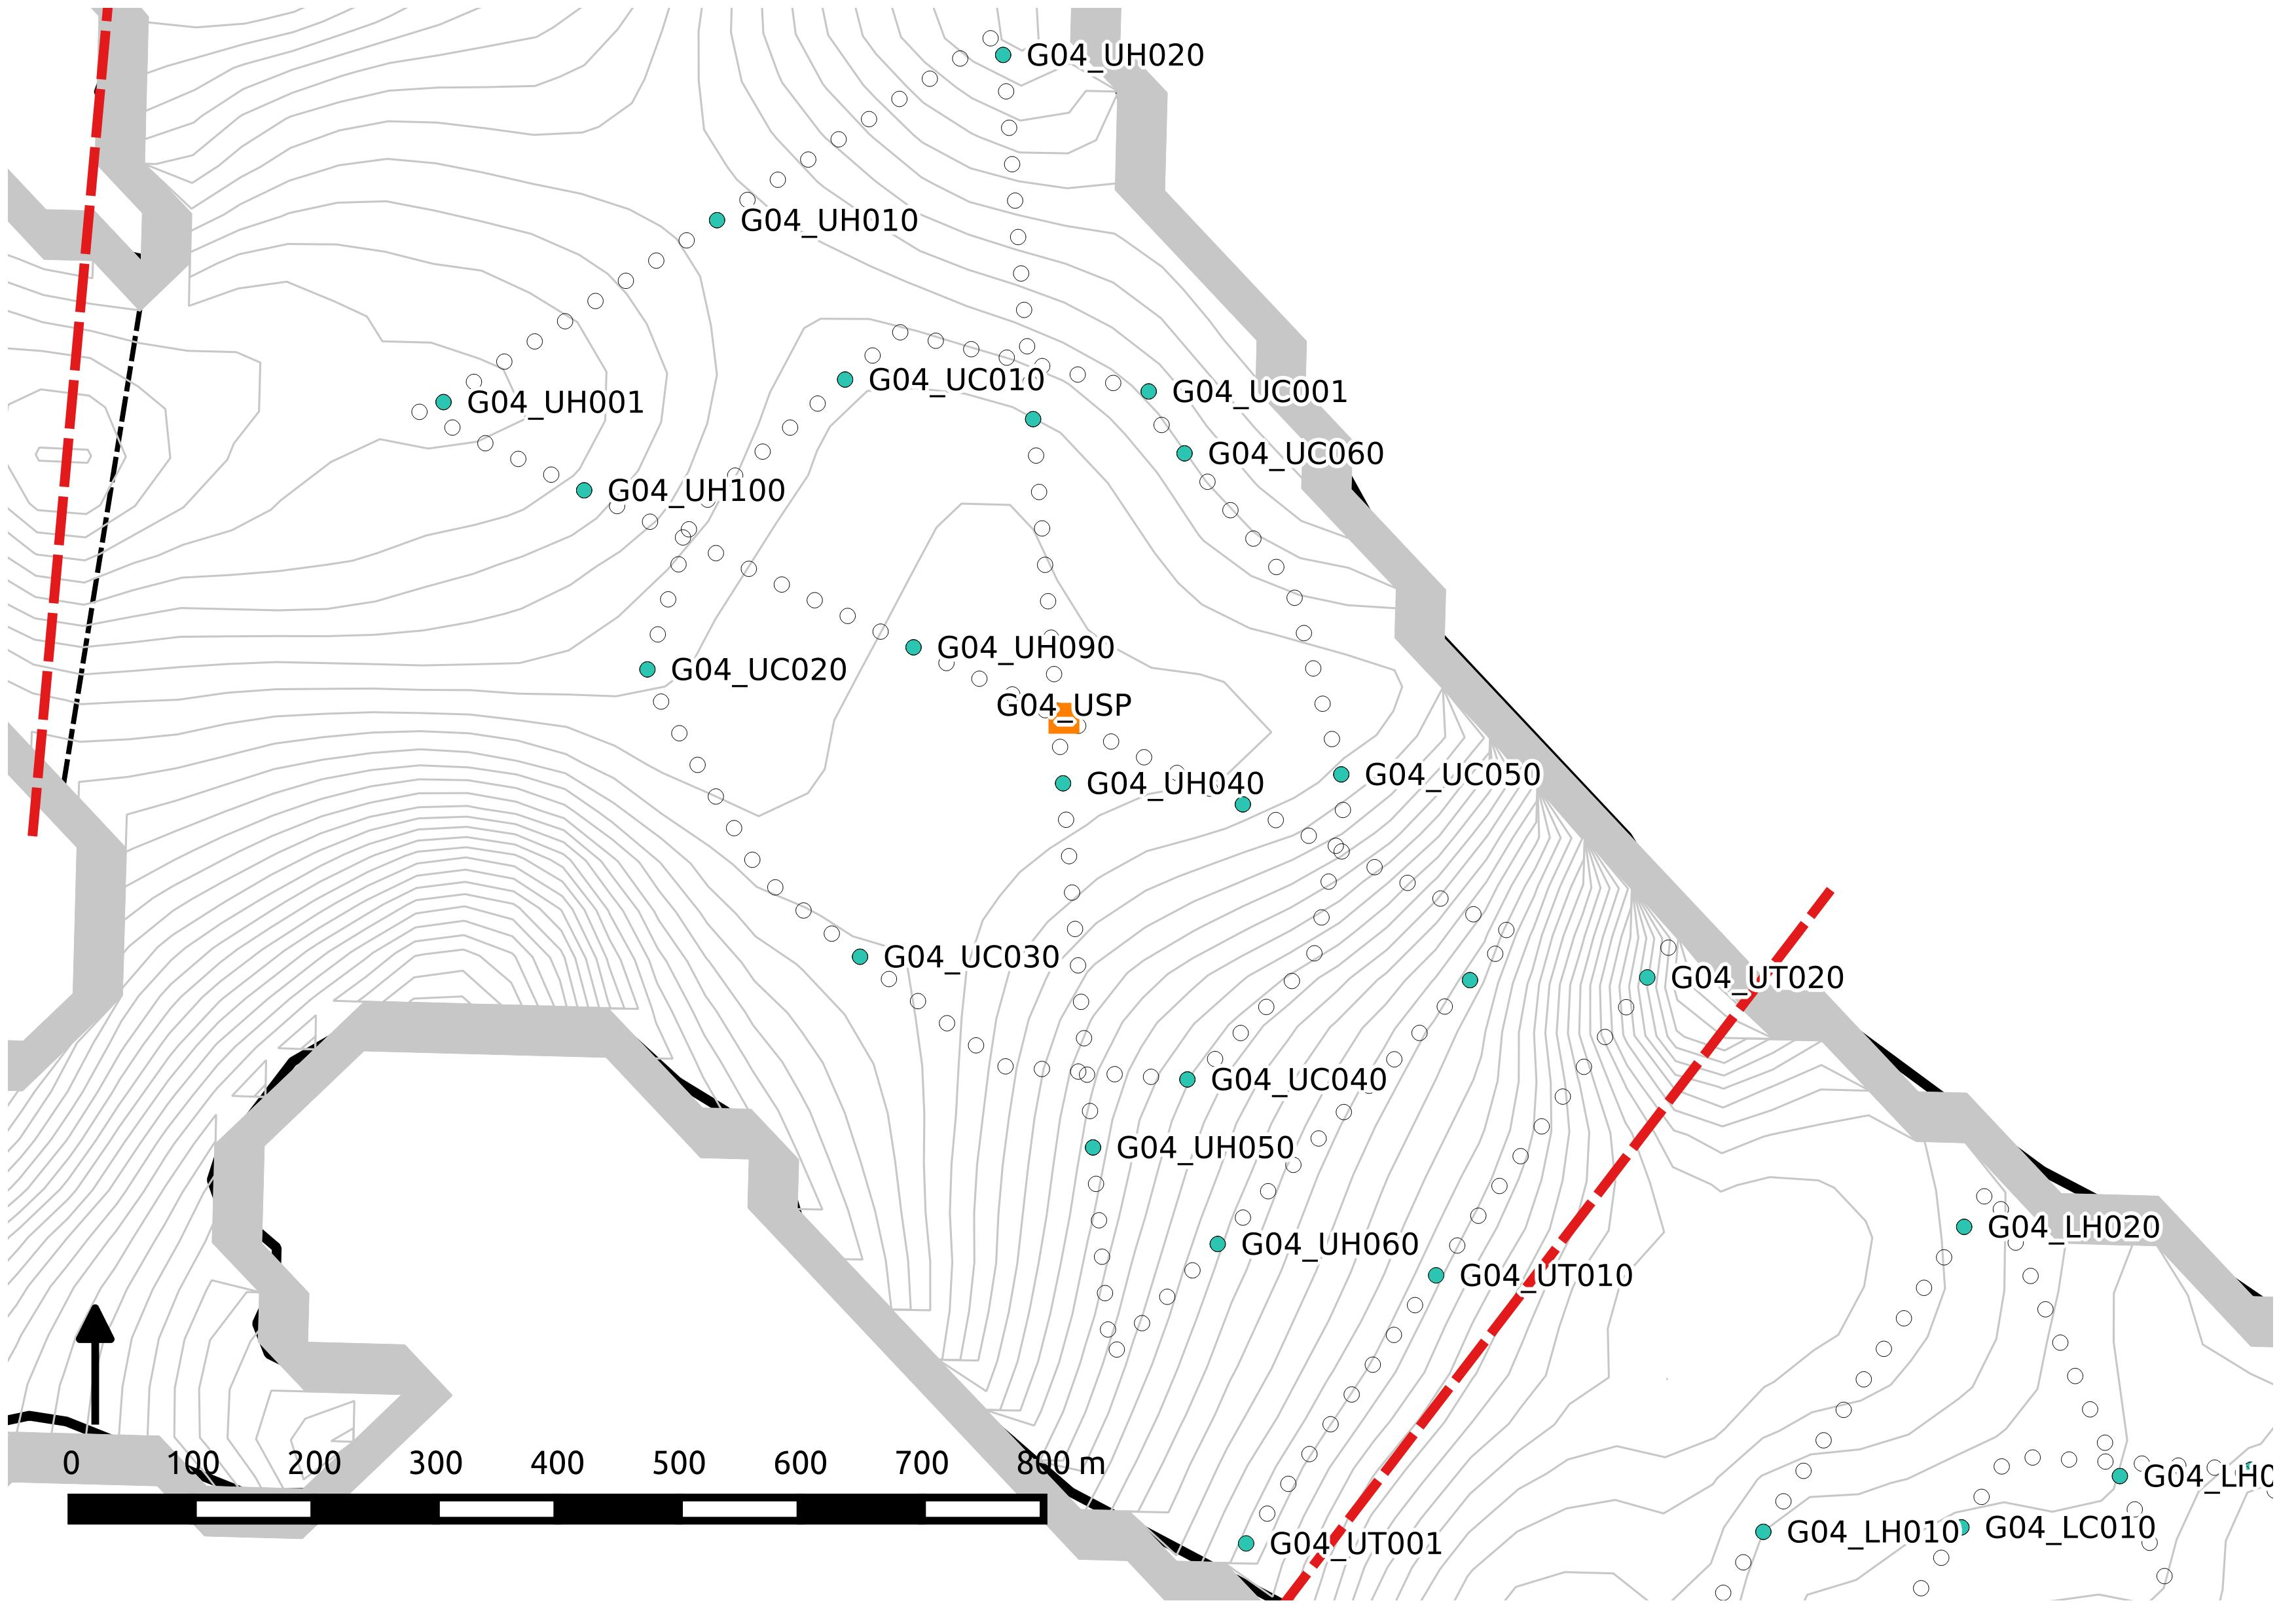
\includegraphics[height = 0.45\textheight]{G04_UH.jpeg}}\\
\fbox{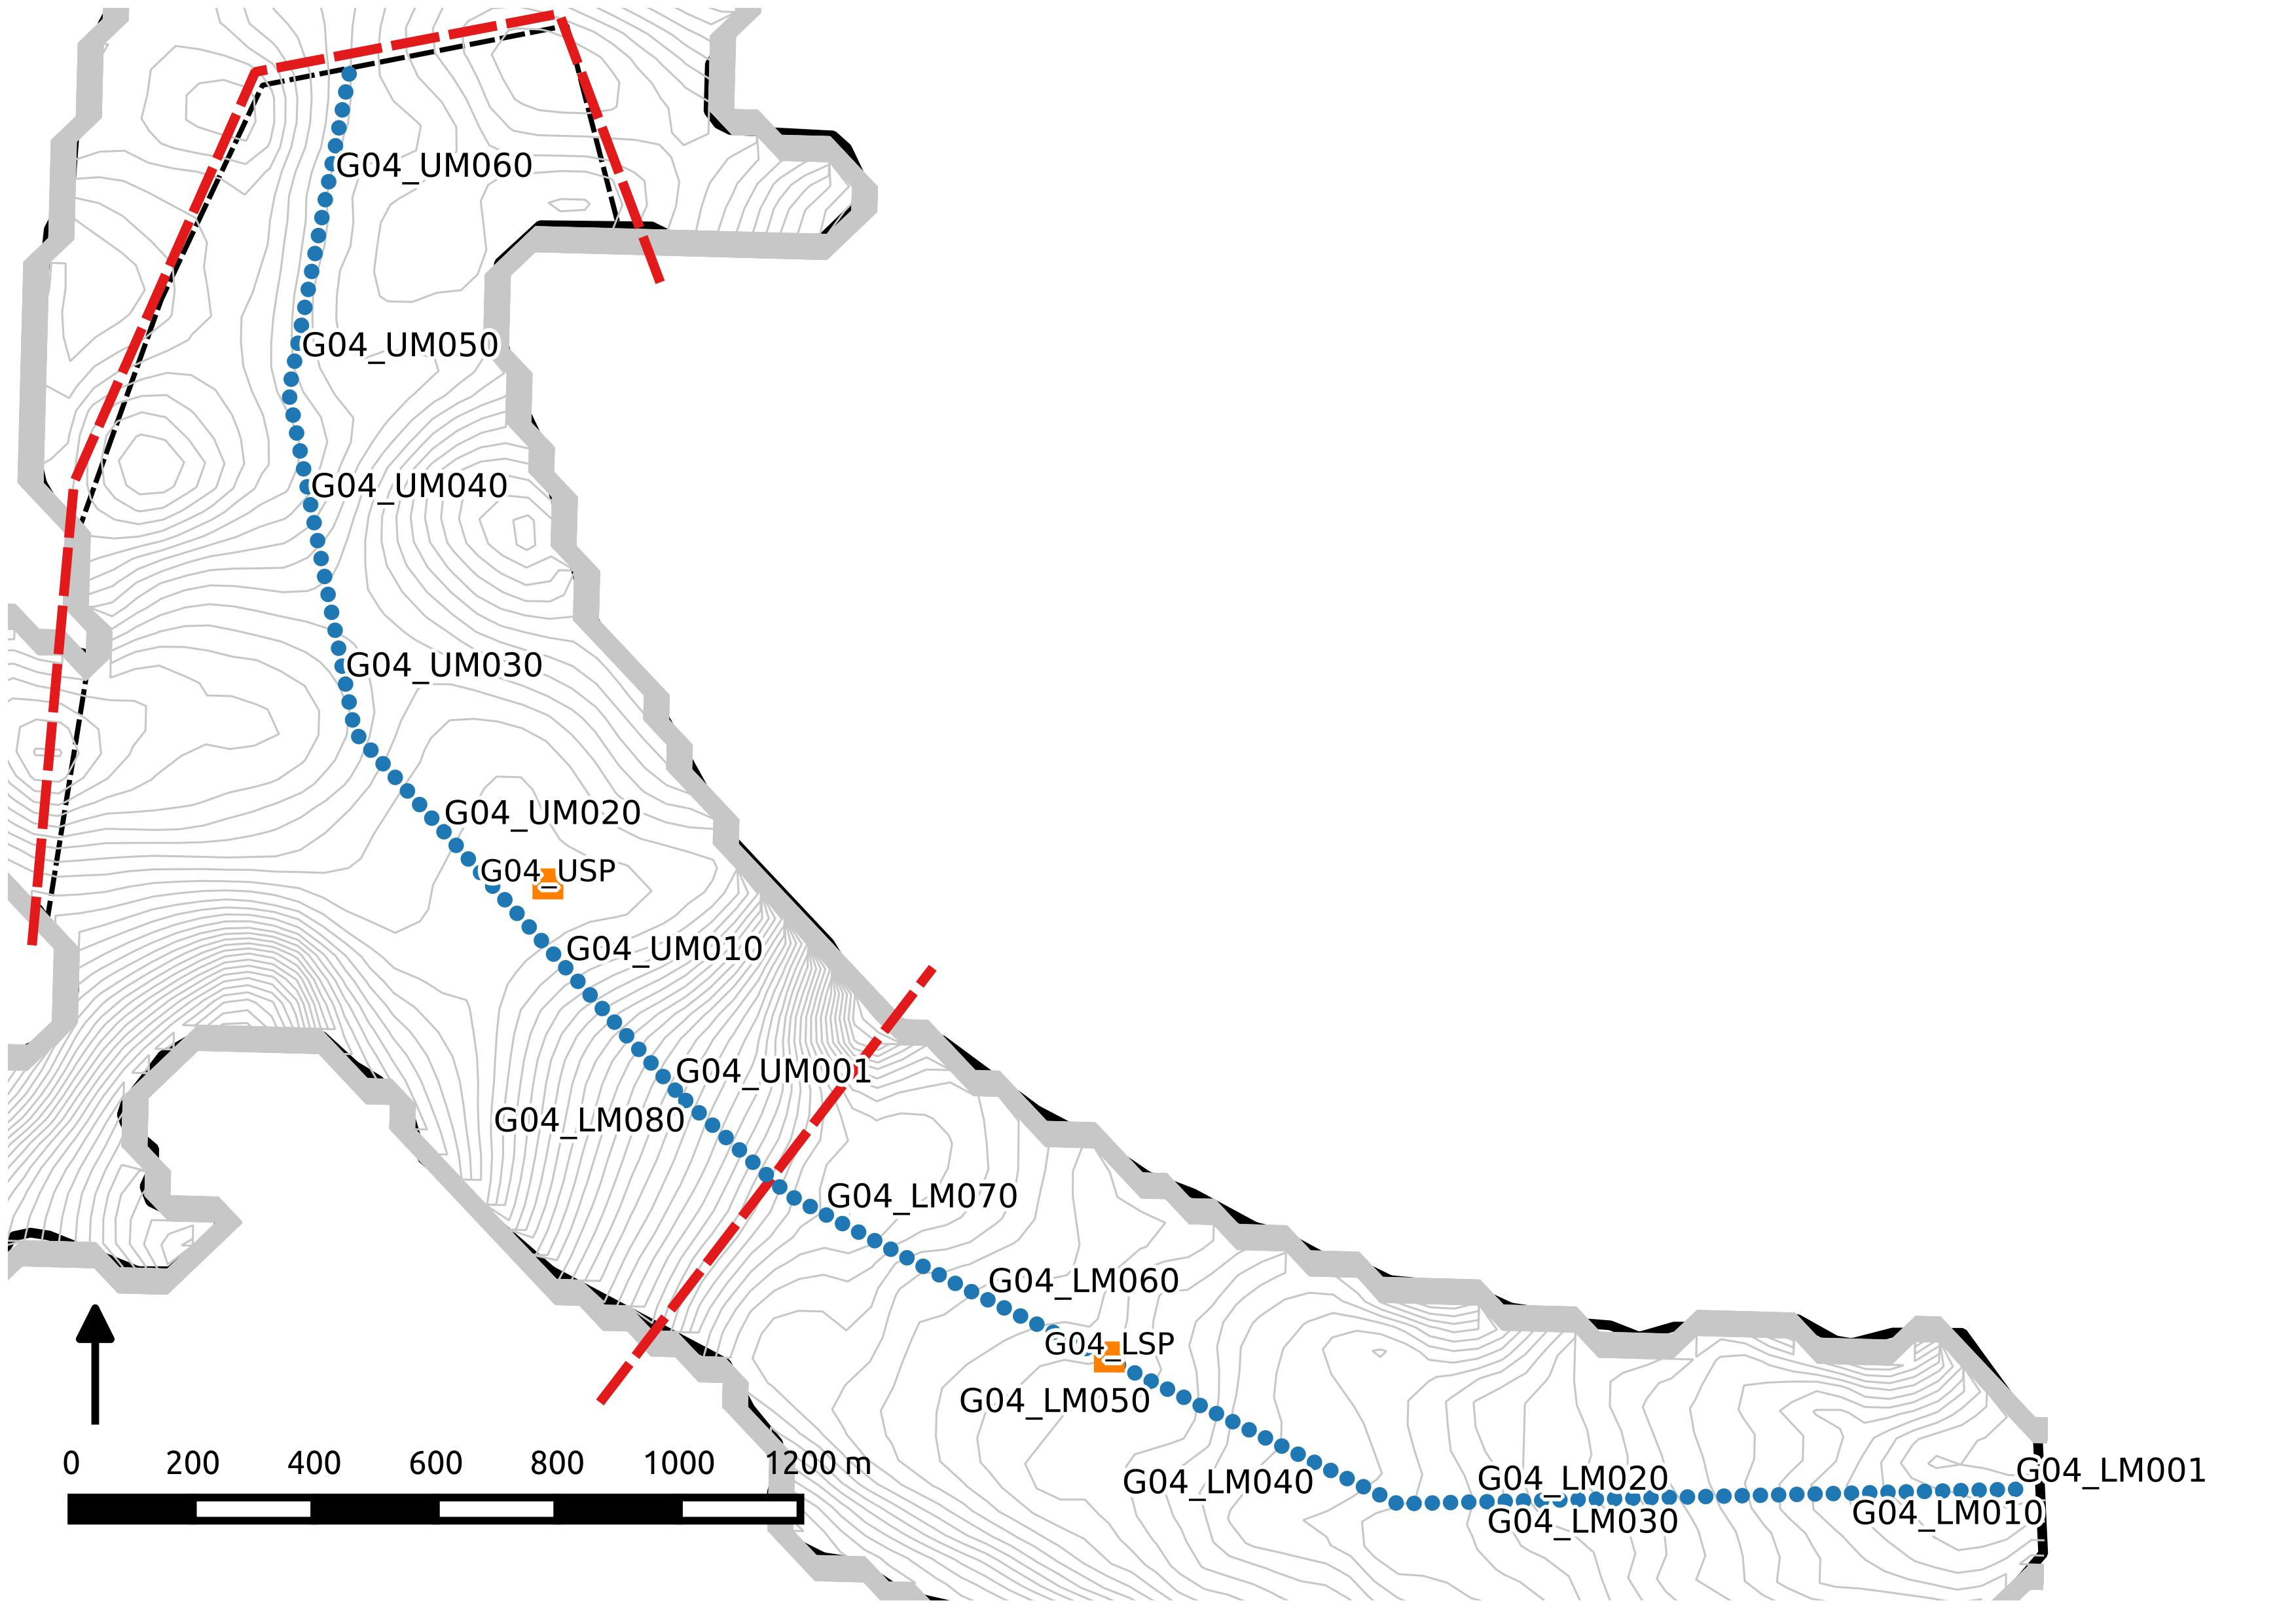
\includegraphics[height = 0.45\textheight]{G04_M.jpeg}}\\
\fbox{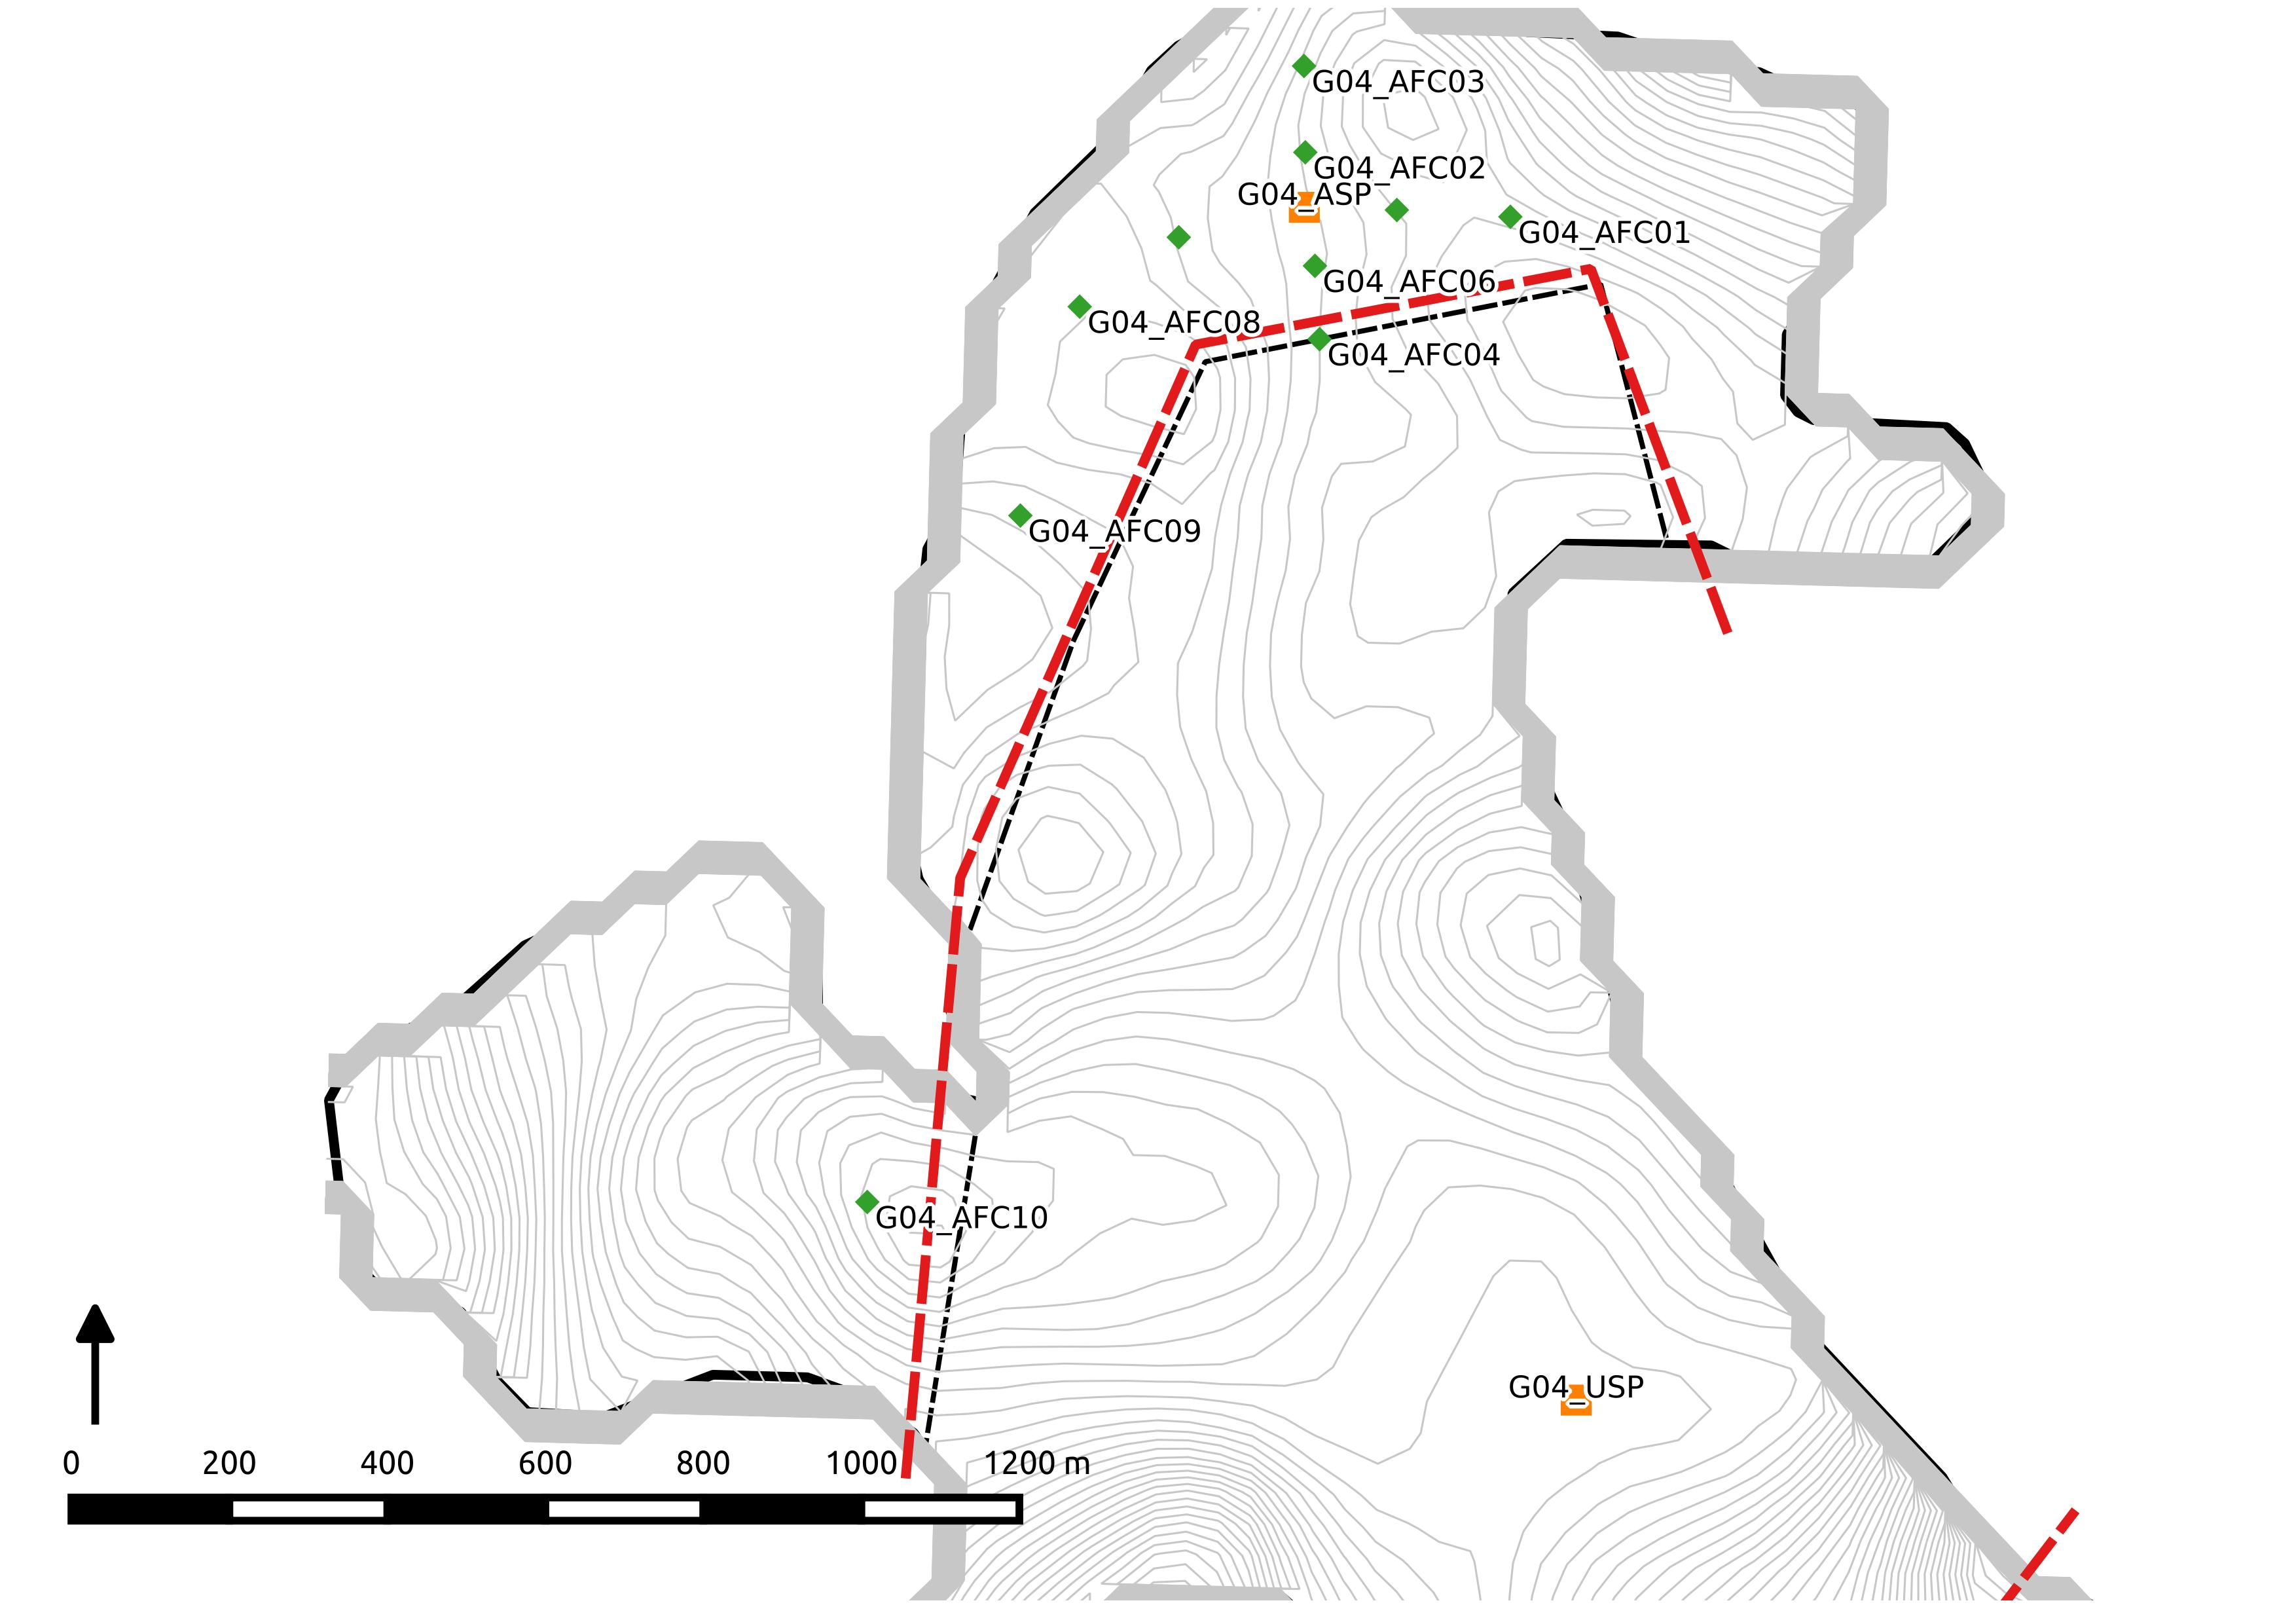
\includegraphics[height = 0.45\textheight]{G04_A.jpeg}}\\

\pagebreak
\noindent \large{\textbf{Glacier 2}}\\
\fbox{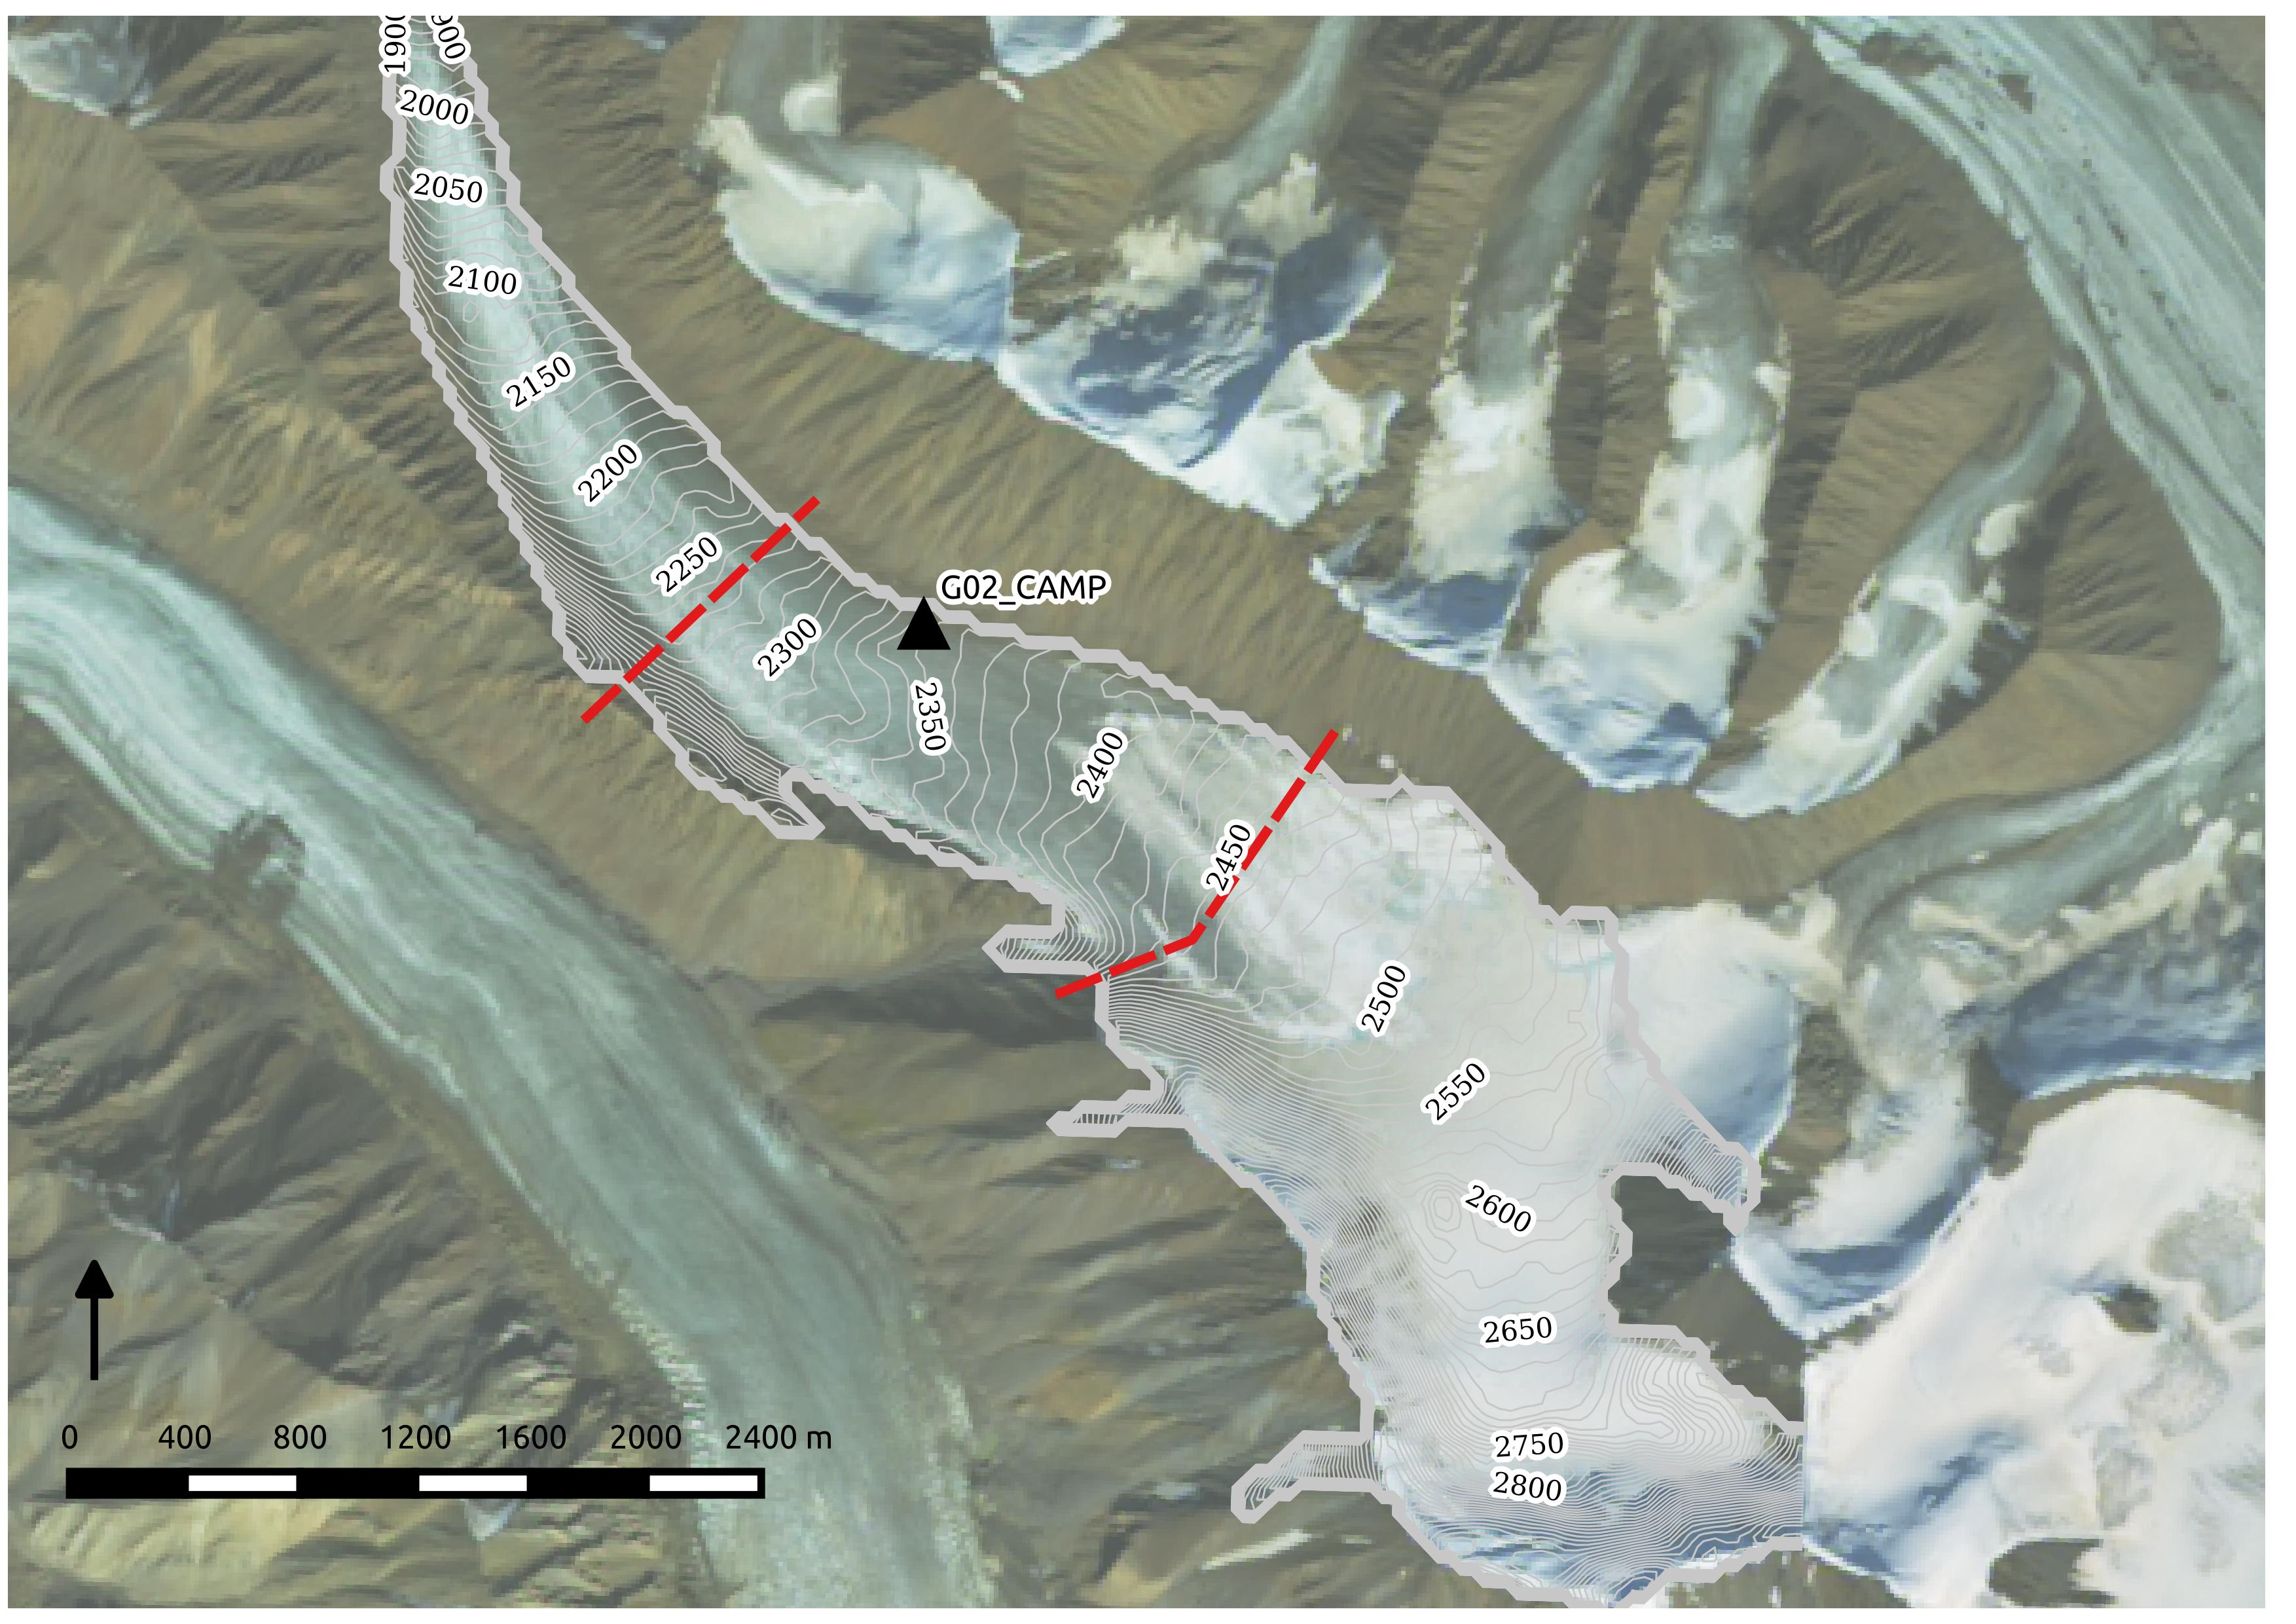
\includegraphics[height = 0.45\textheight]{G02_topo.jpeg}}\\
\fbox{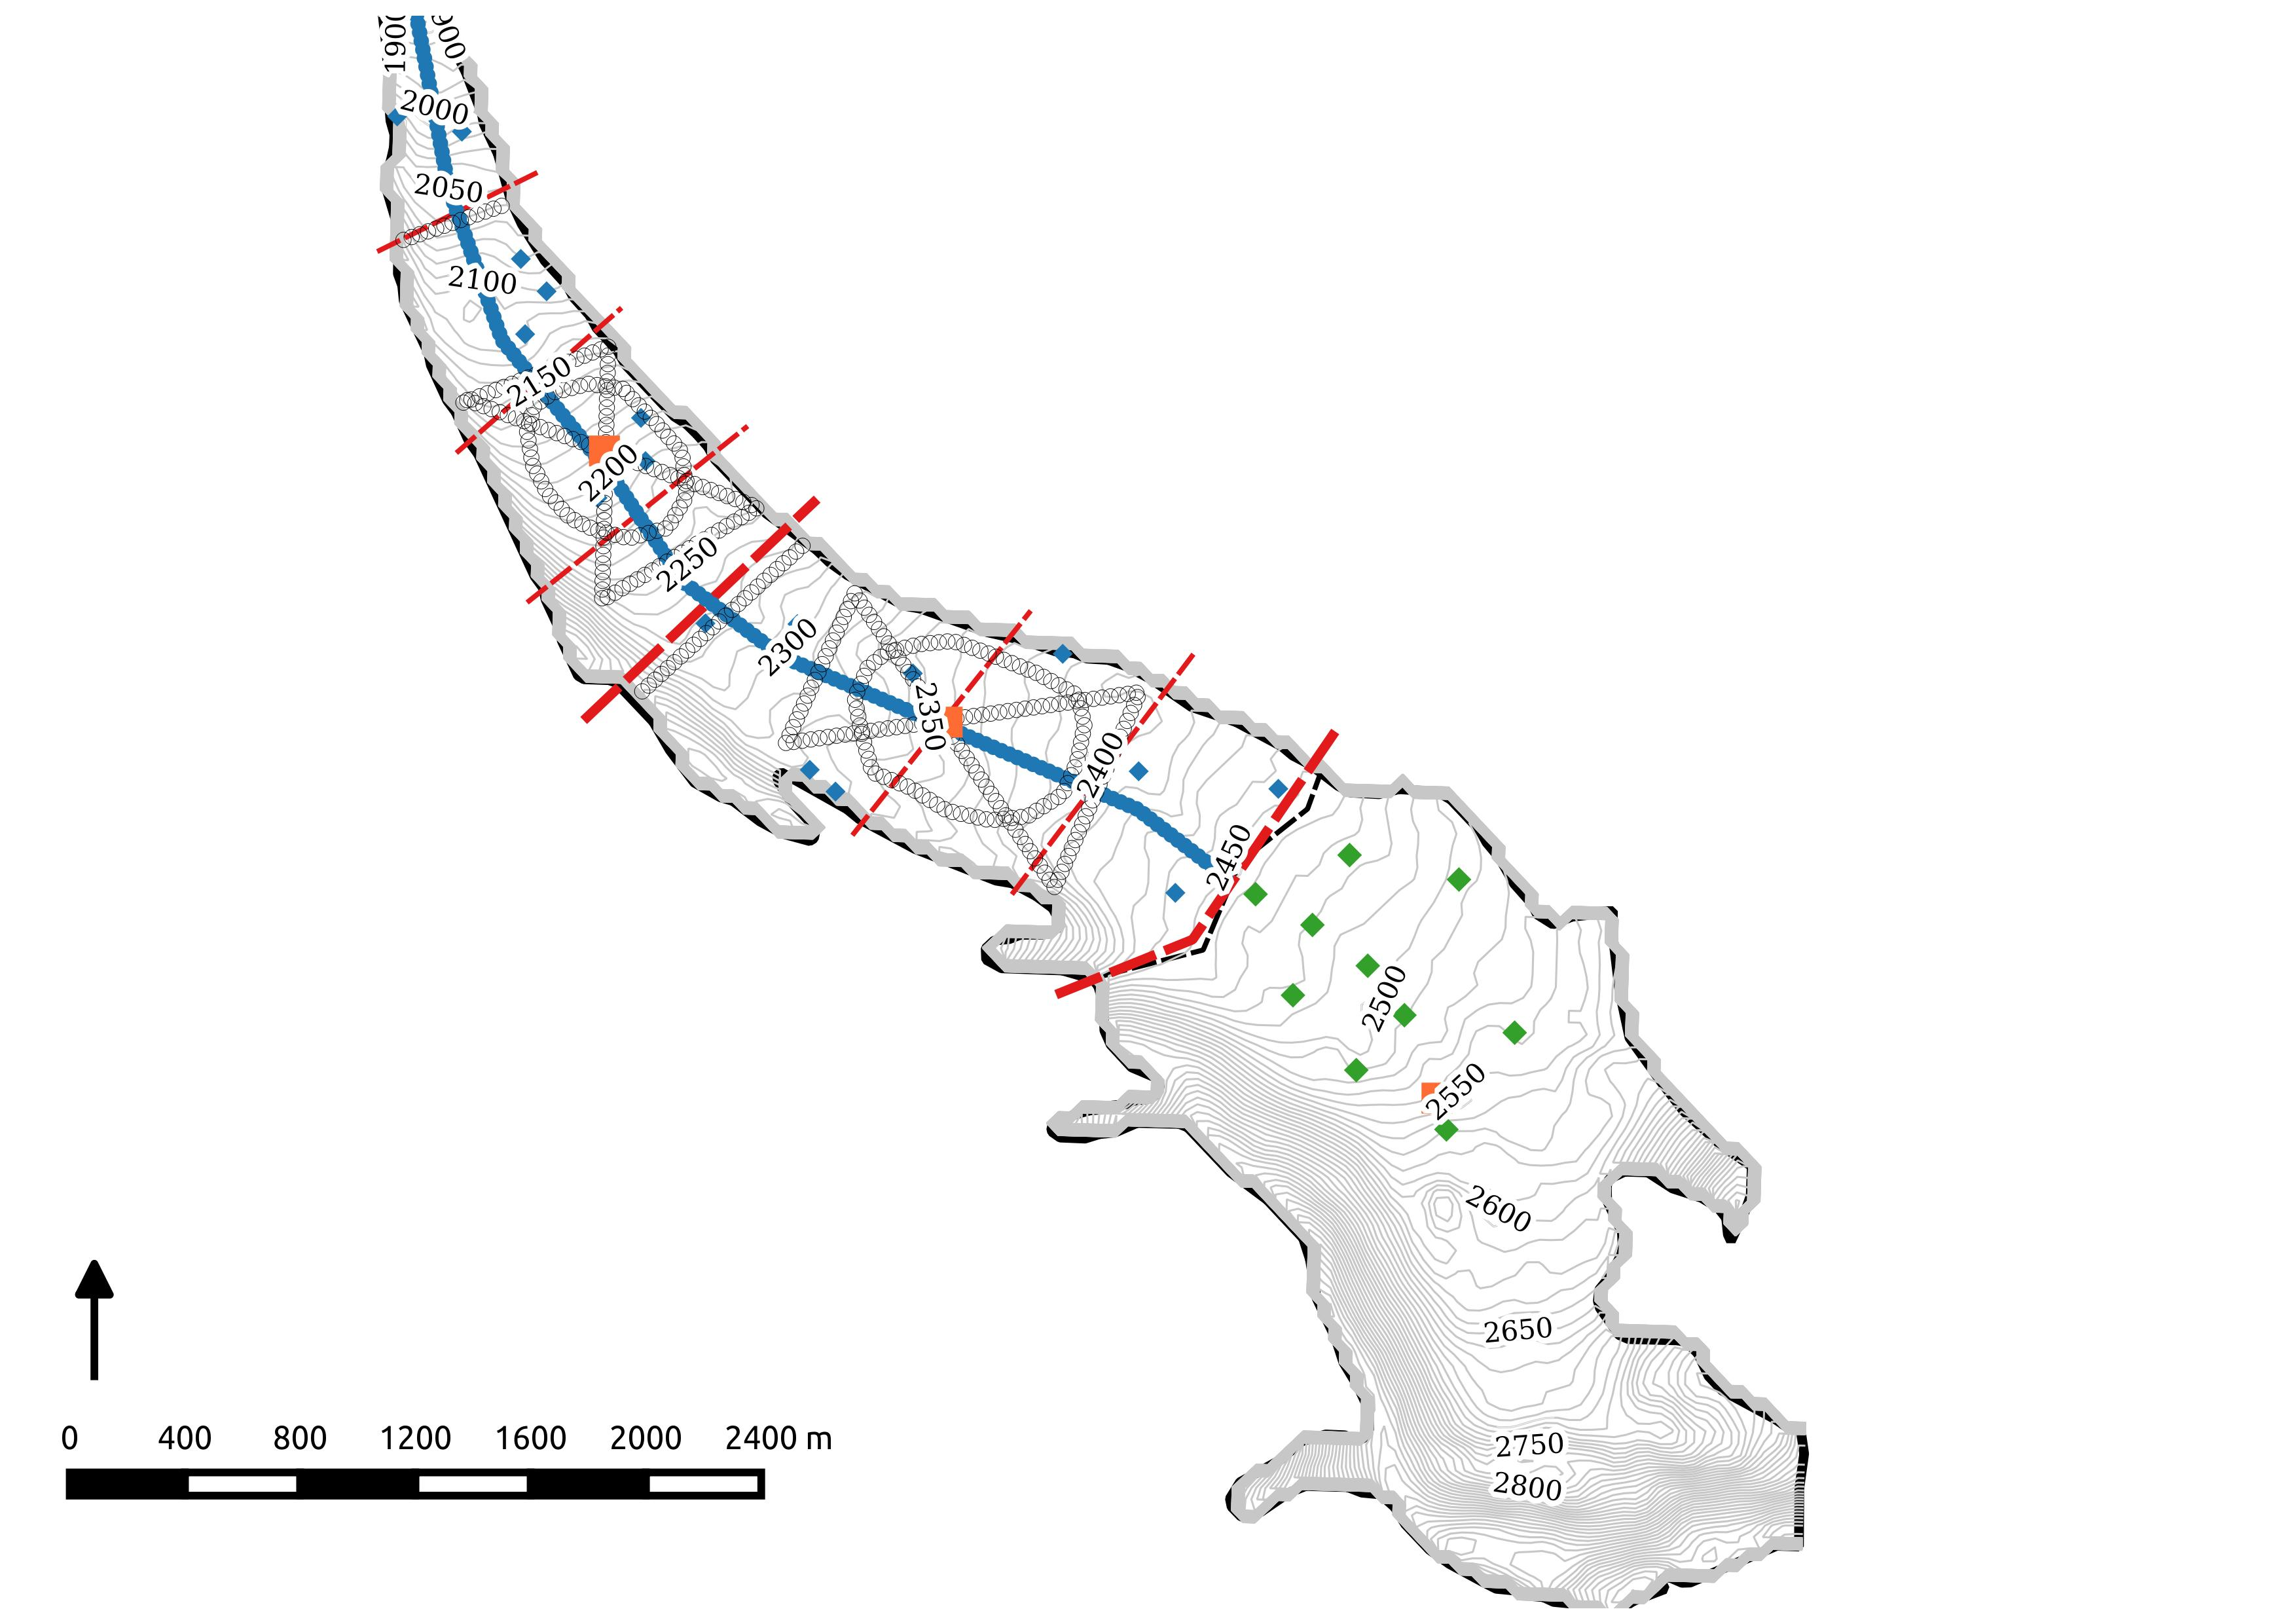
\includegraphics[height = 0.45\textheight]{G02_Overview.jpeg}}\\
\fbox{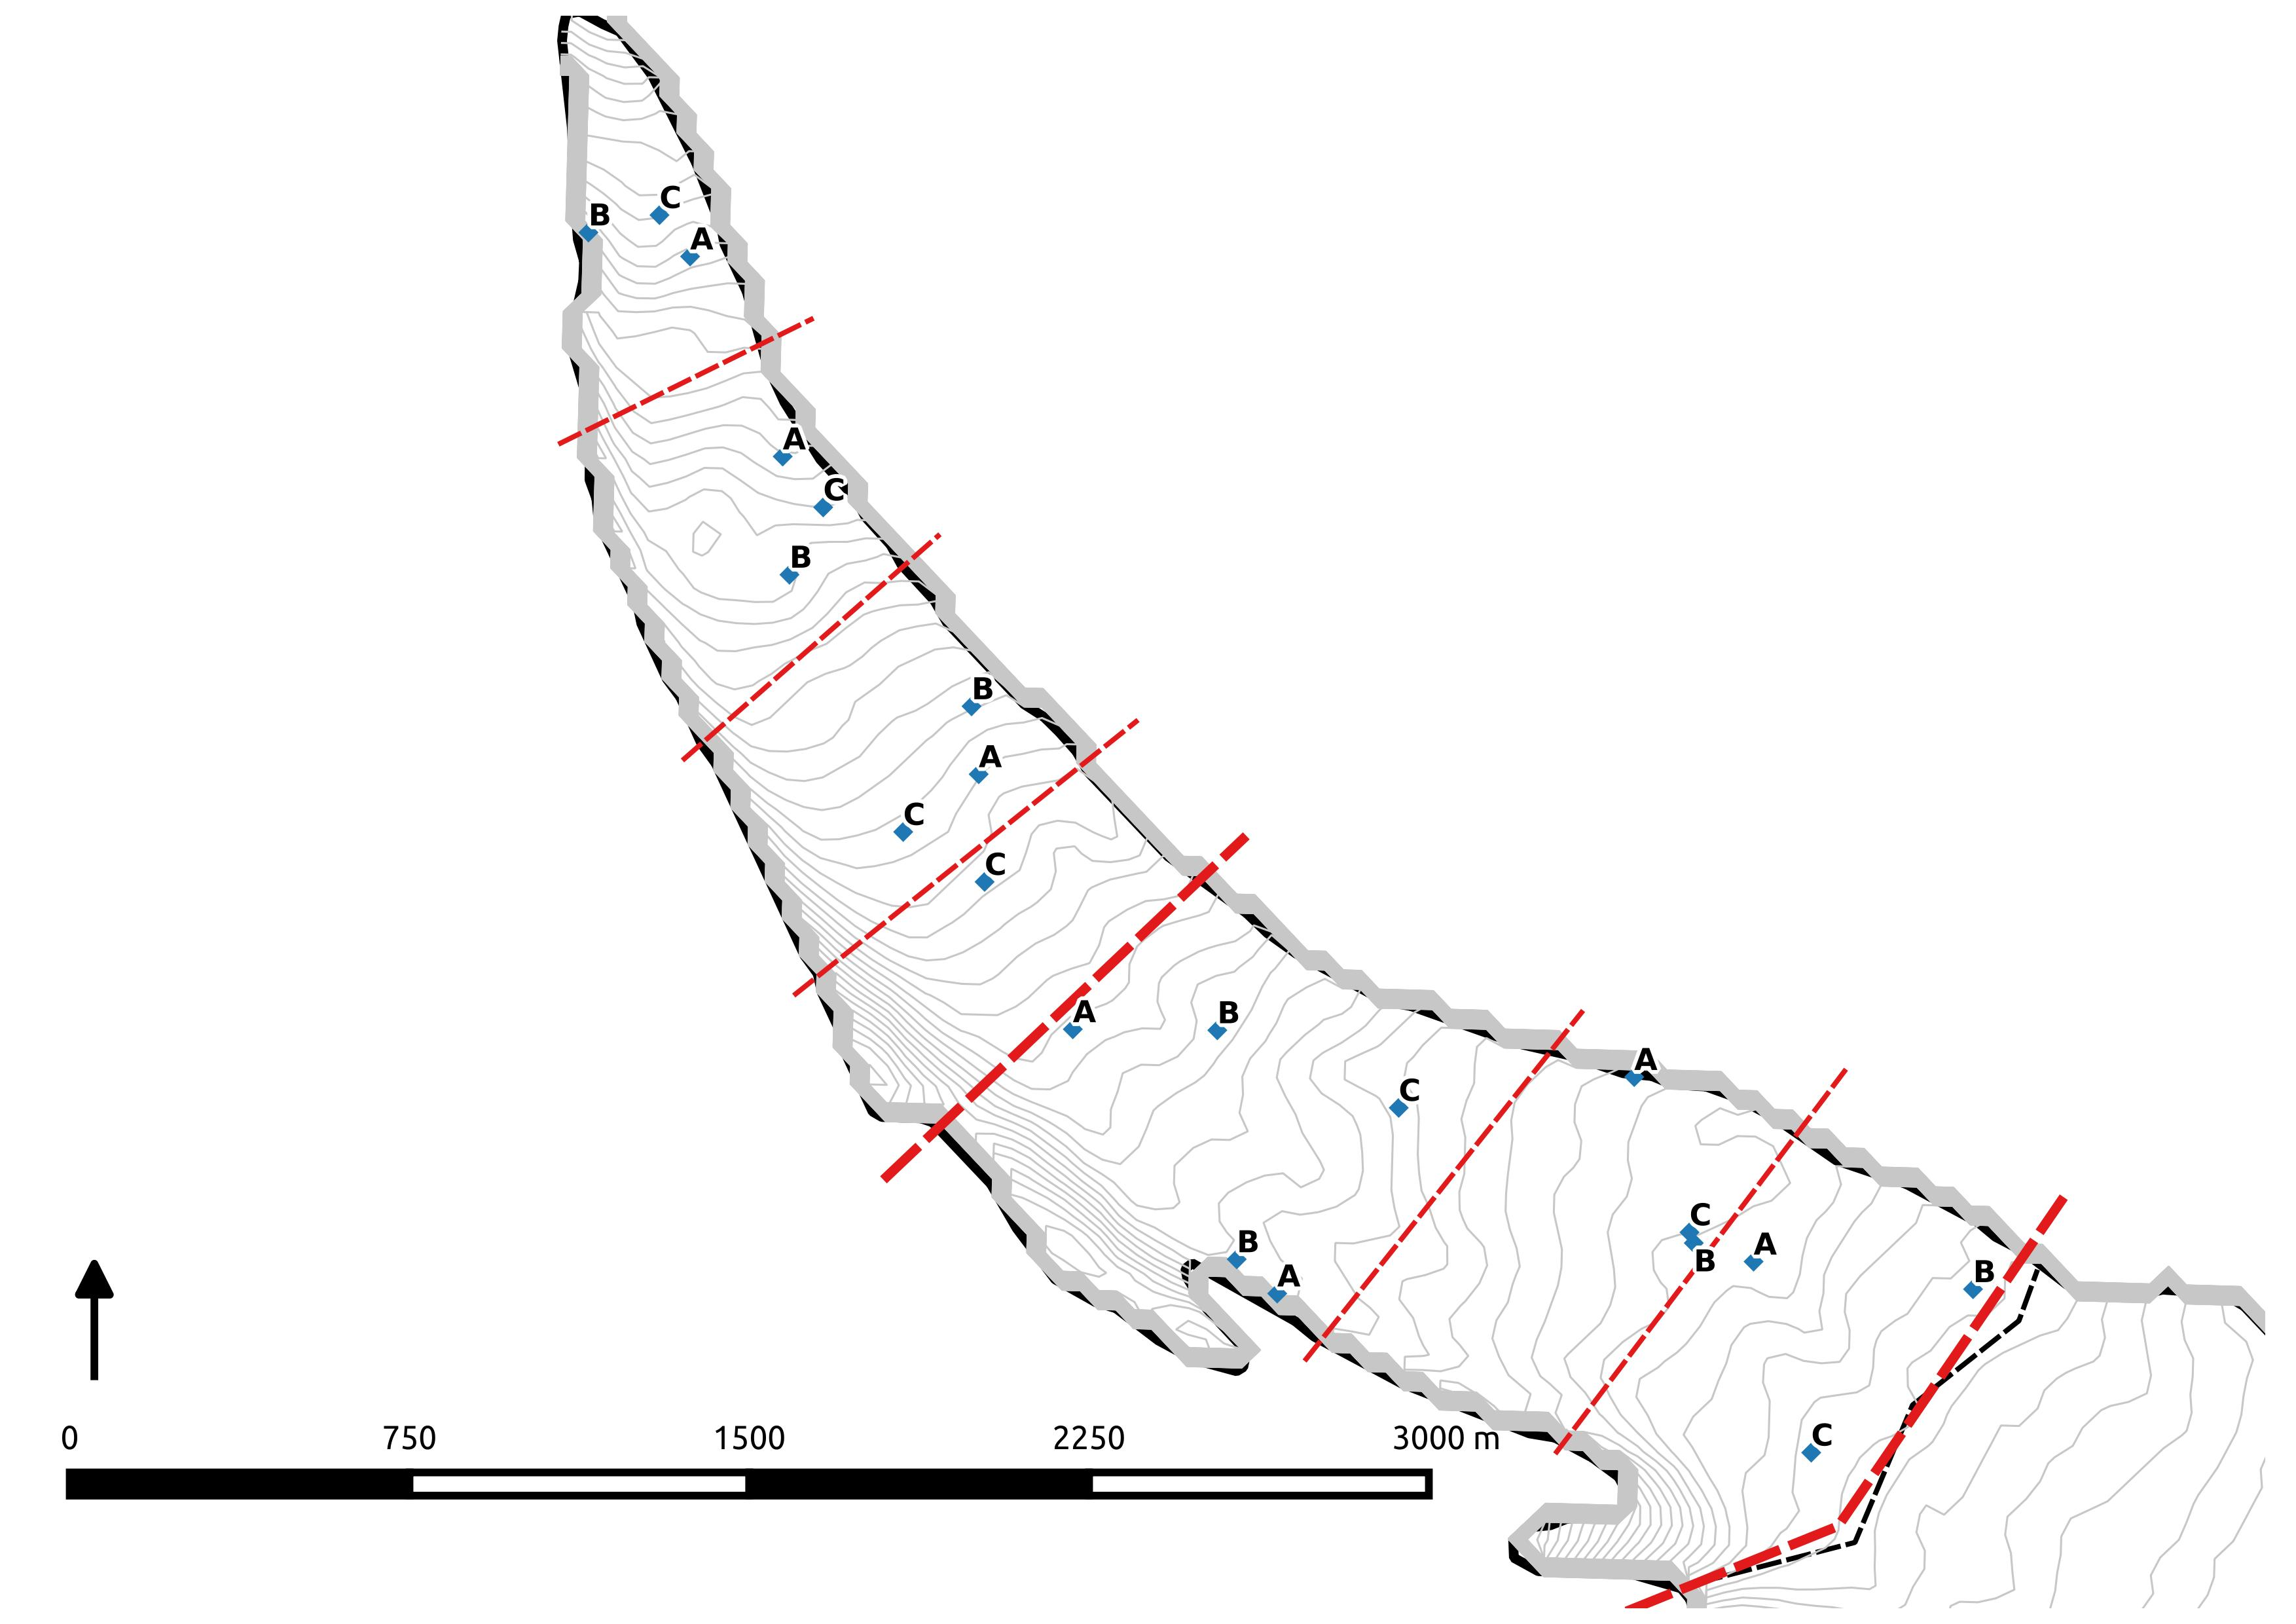
\includegraphics[height = 0.45\textheight]{G02_ZZ.jpeg}}\\
\fbox{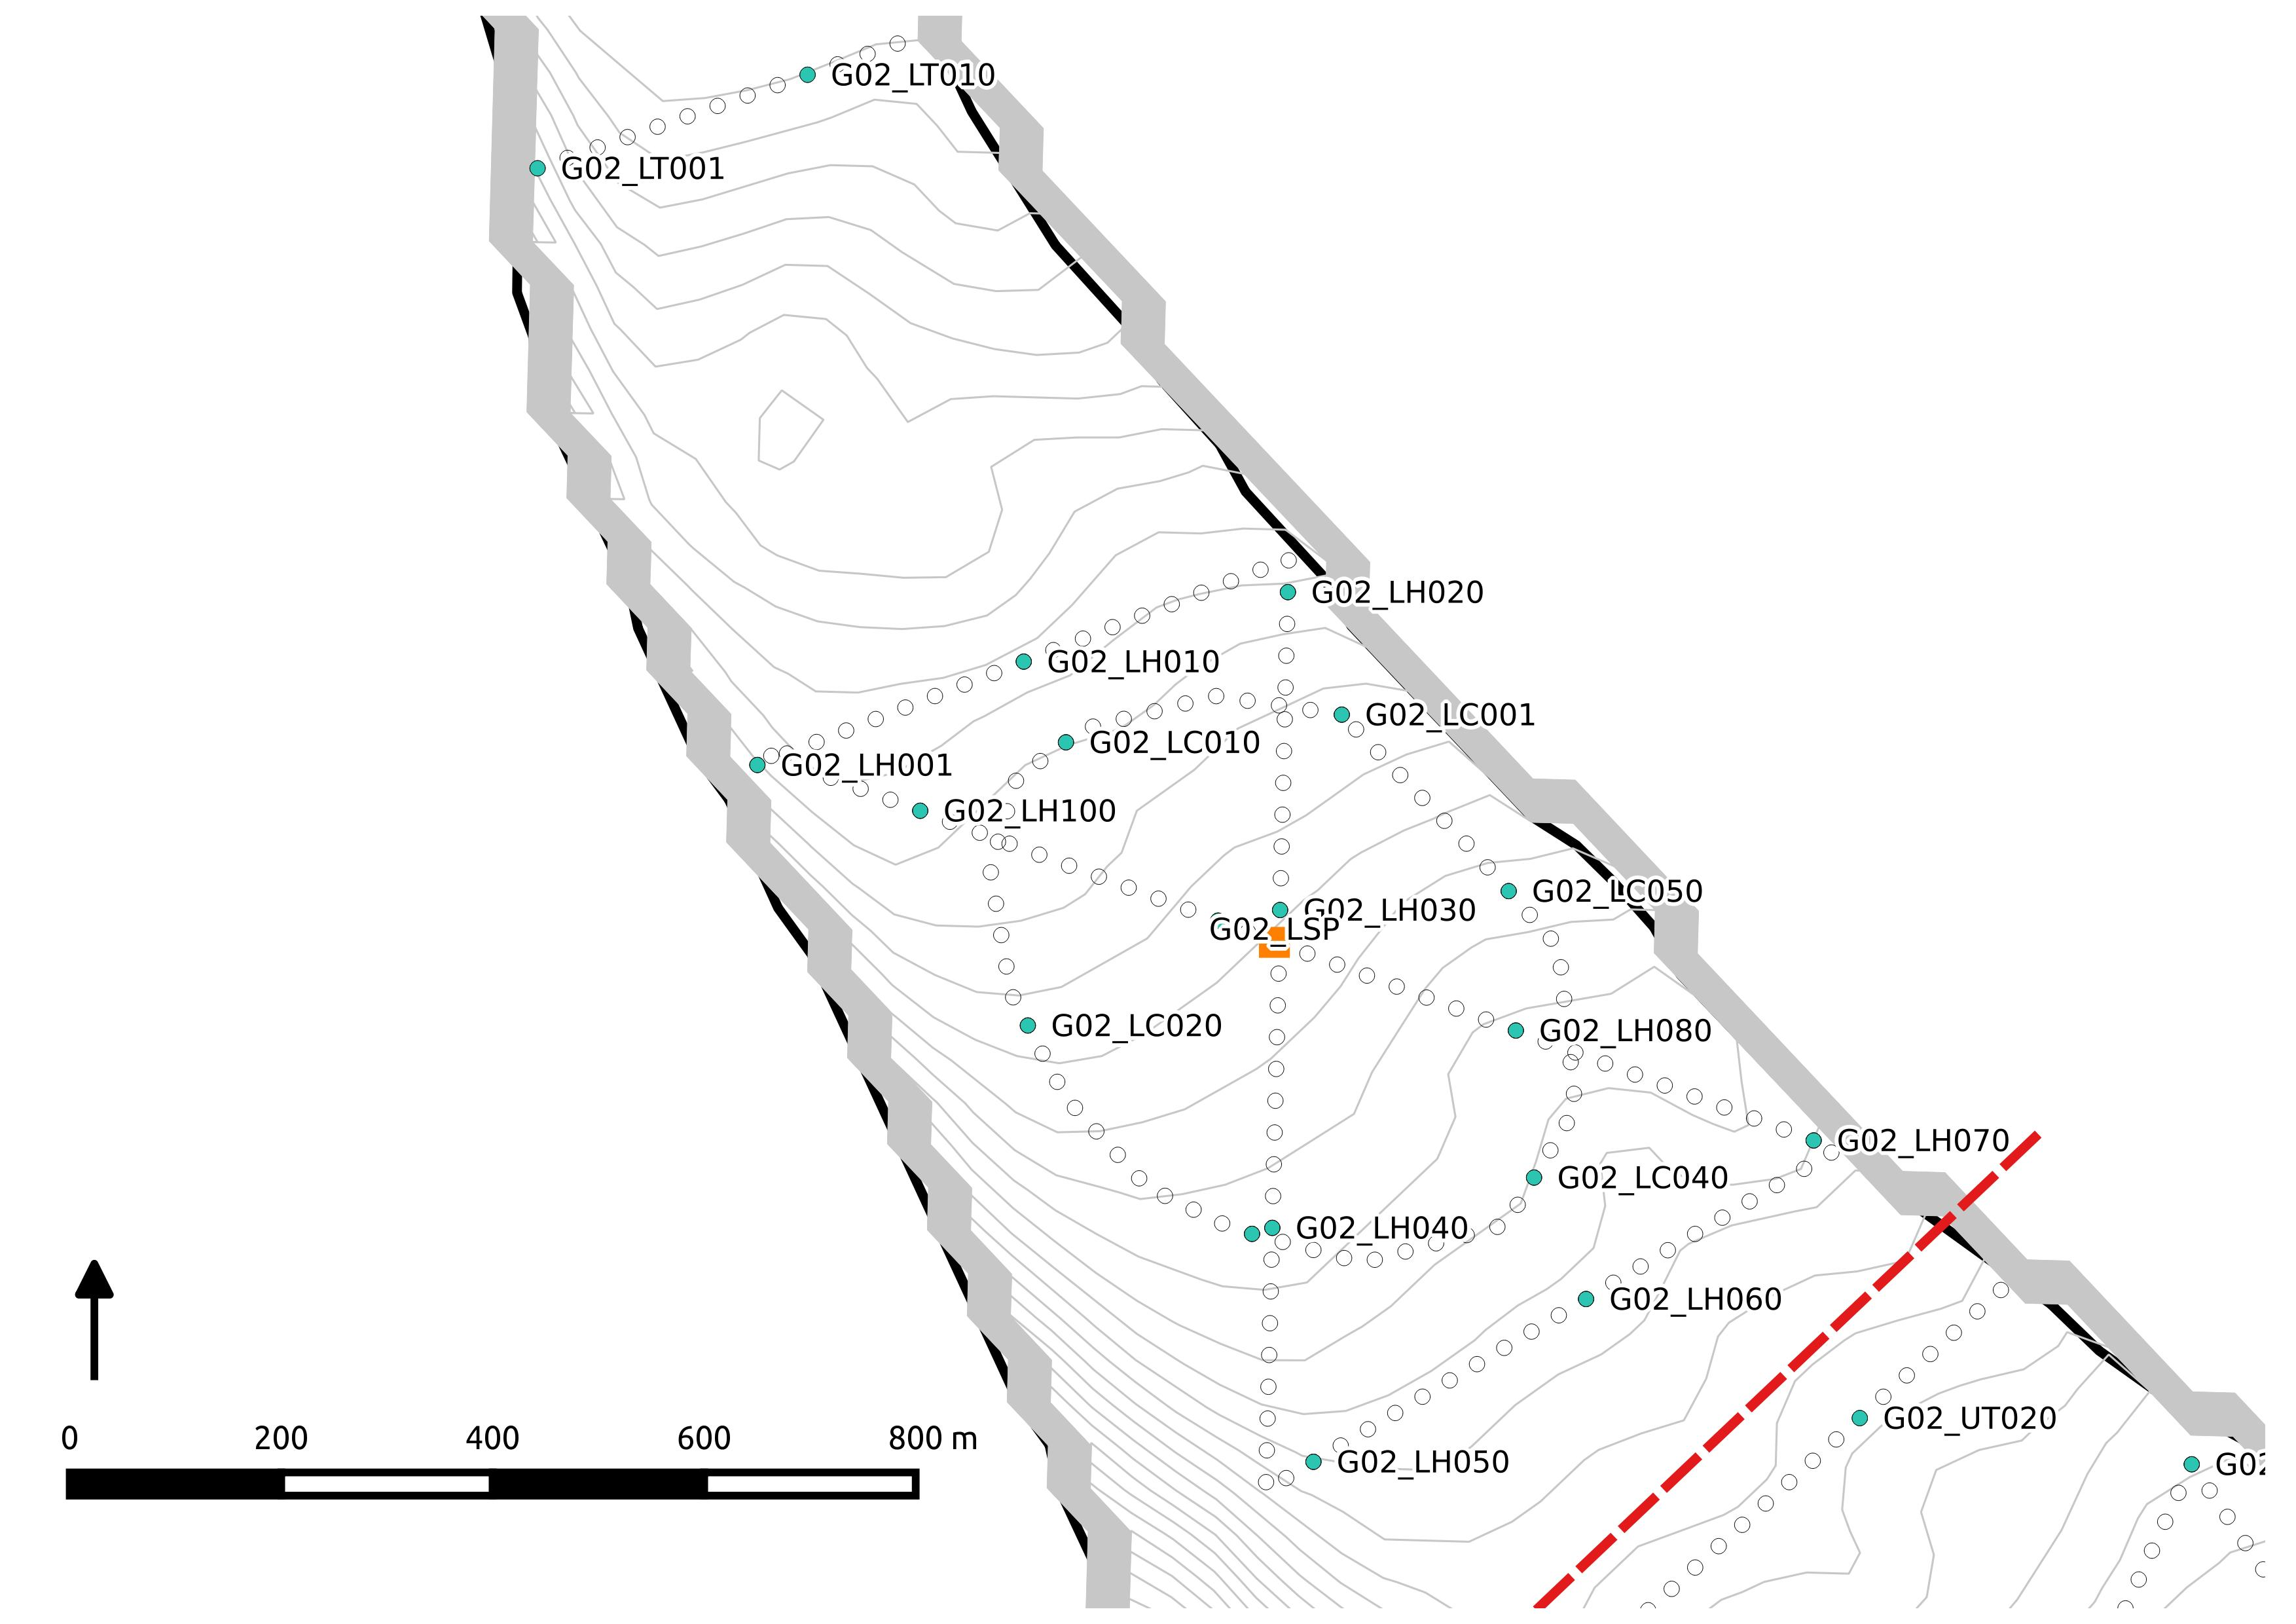
\includegraphics[height = 0.45\textheight]{G02_LH.jpeg}}\\
\fbox{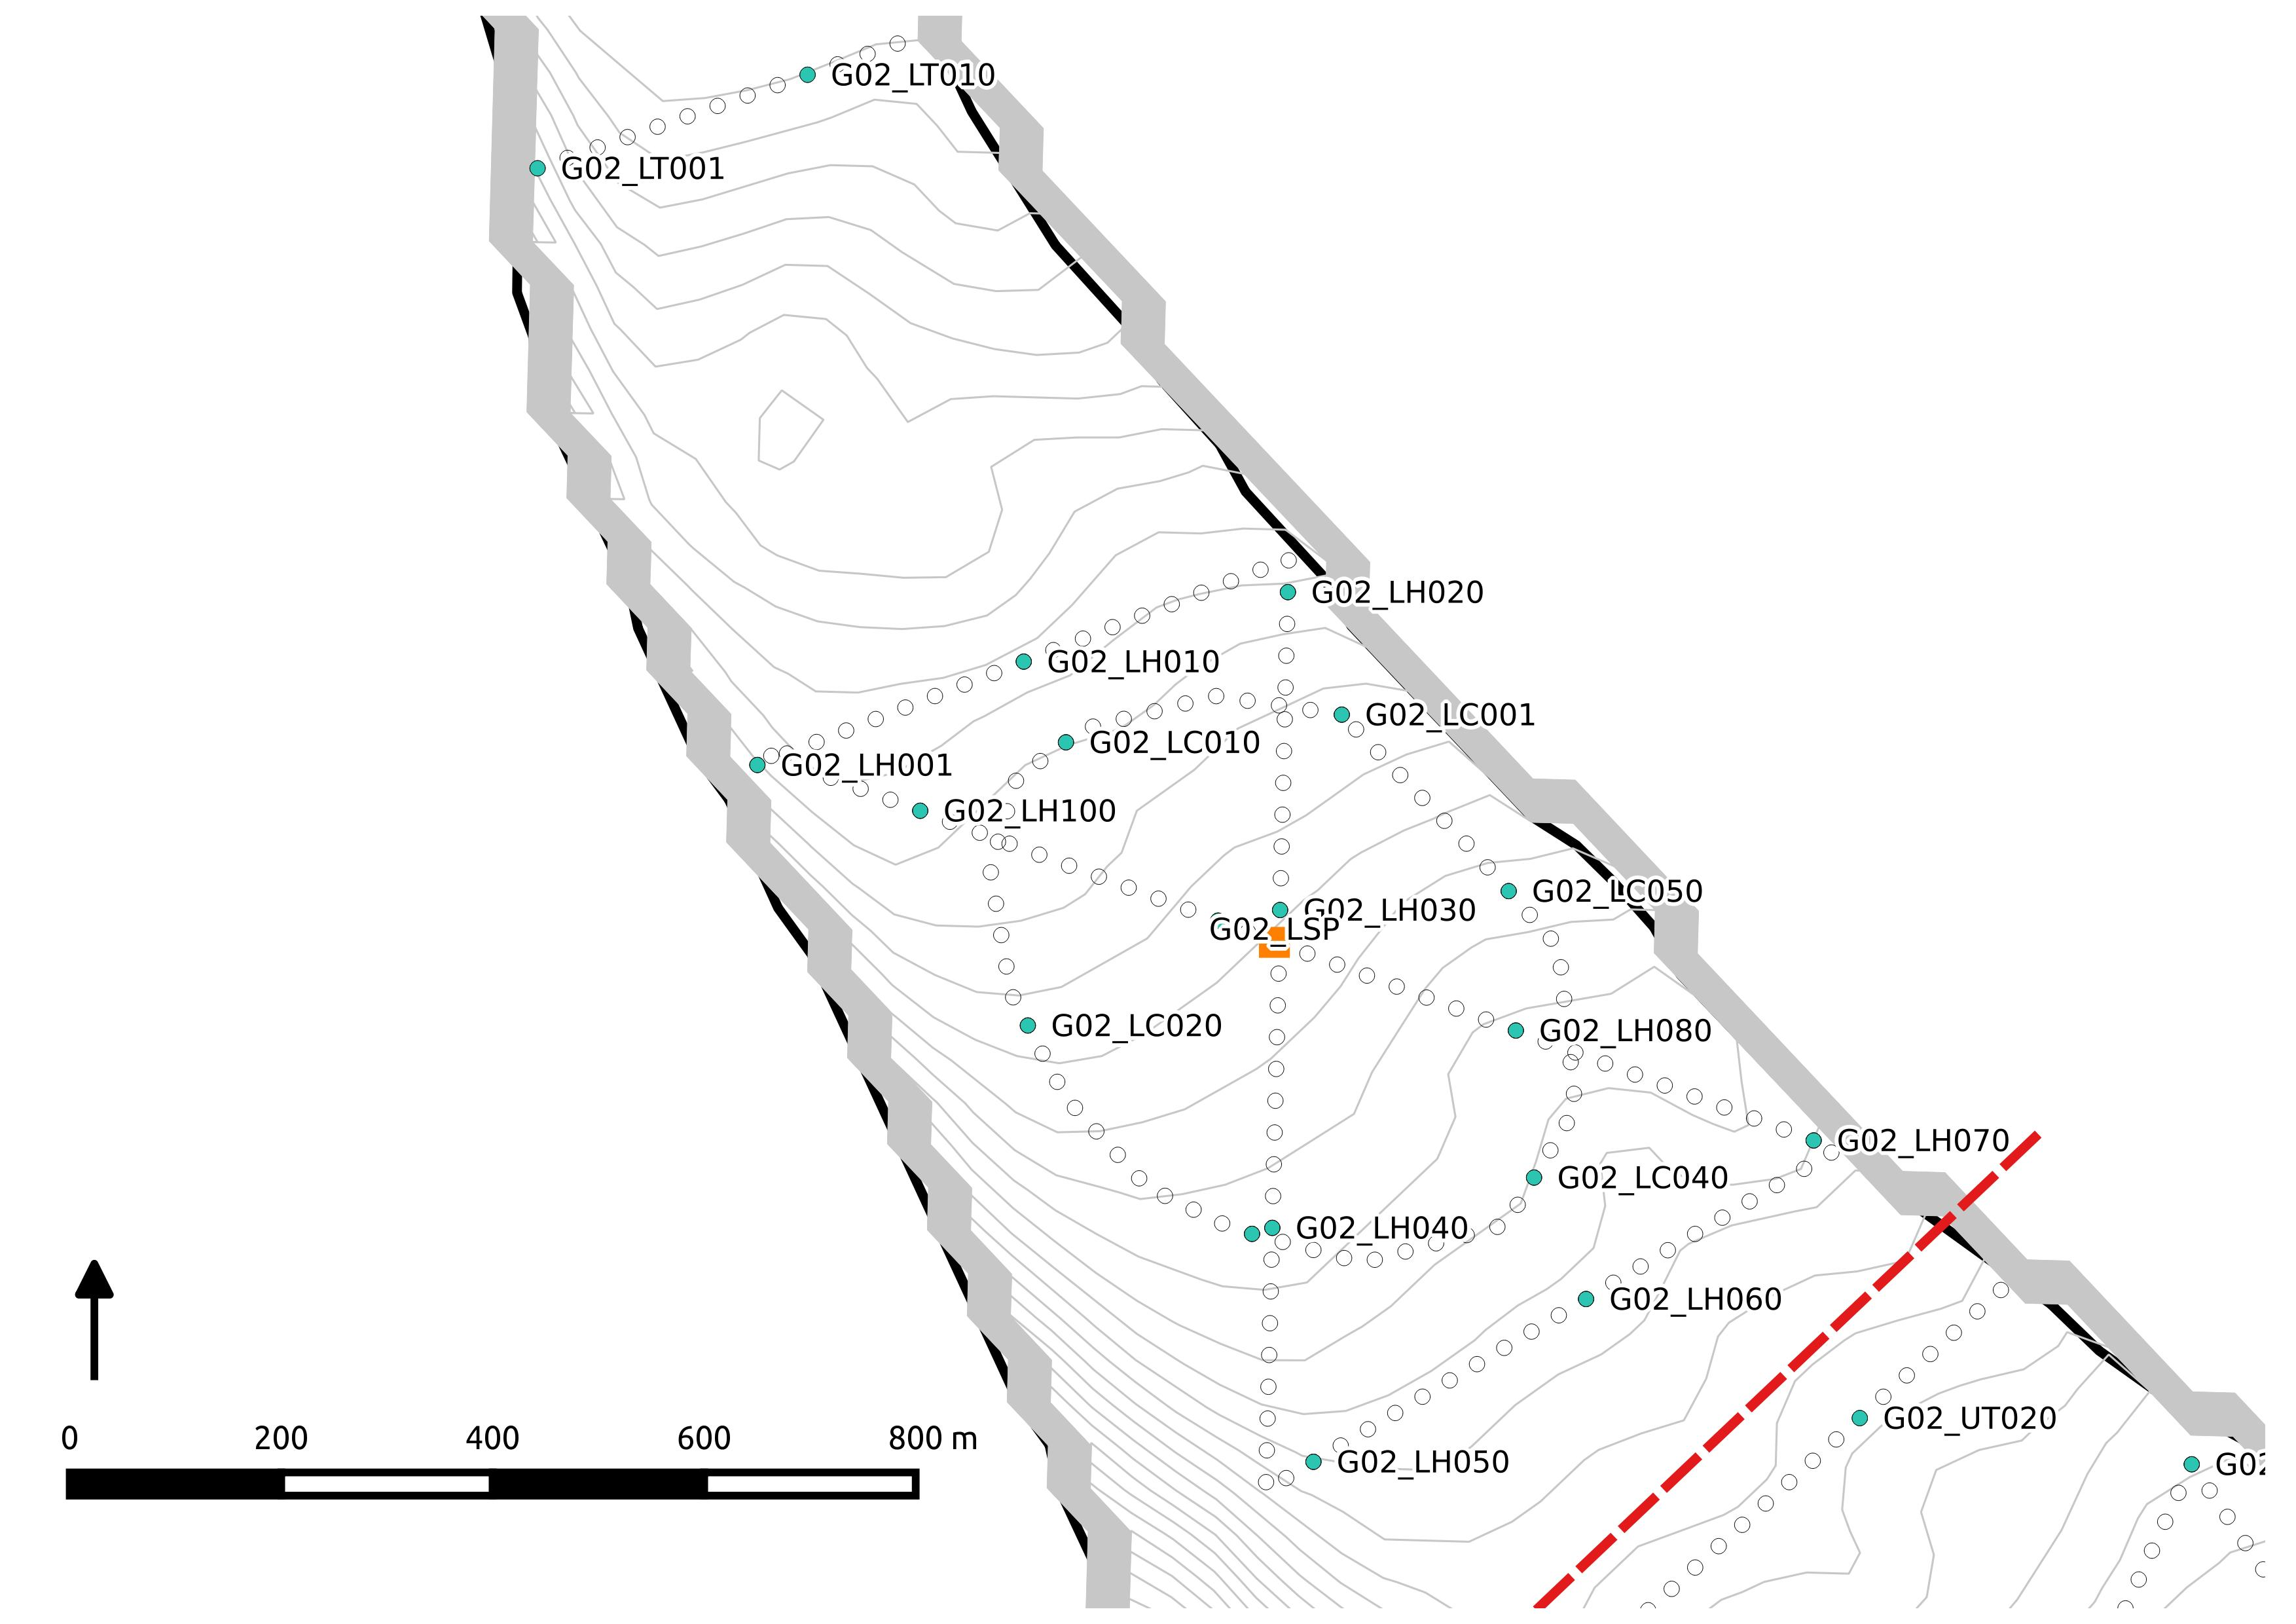
\includegraphics[height = 0.45\textheight]{G02_LH.jpeg}}\\
\fbox{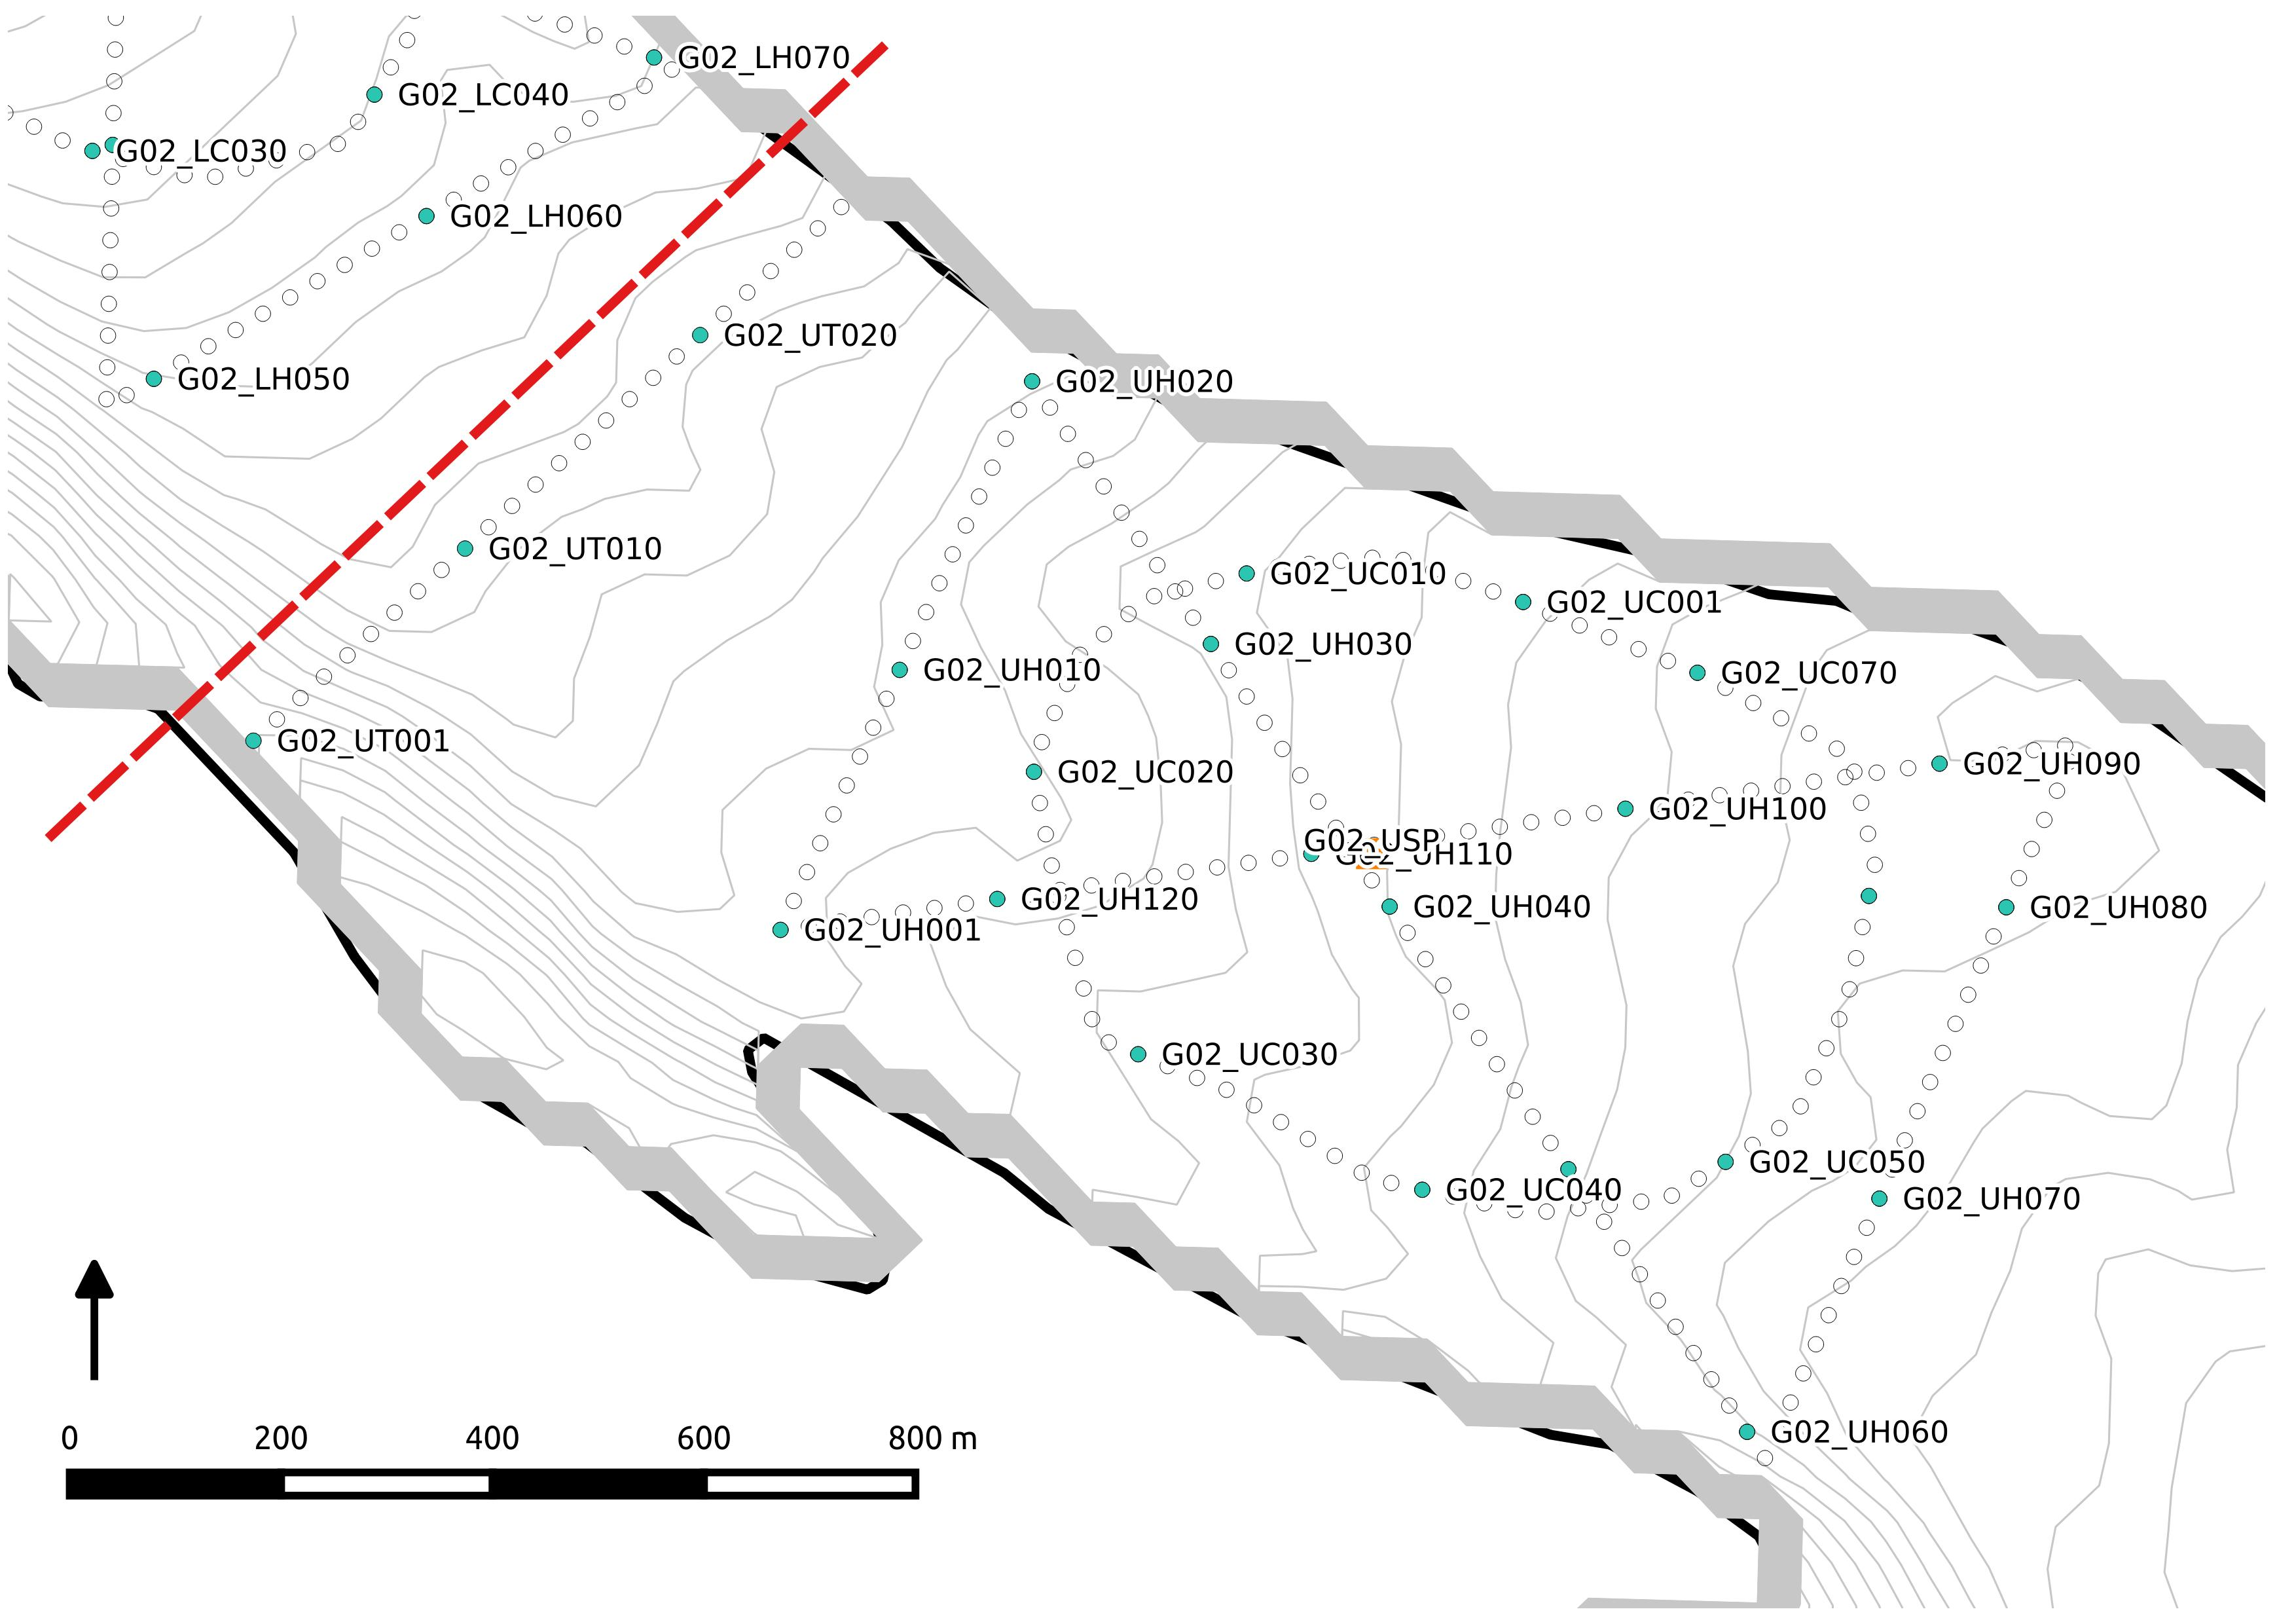
\includegraphics[height = 0.45\textheight]{G02_UH.jpeg}}\\
\fbox{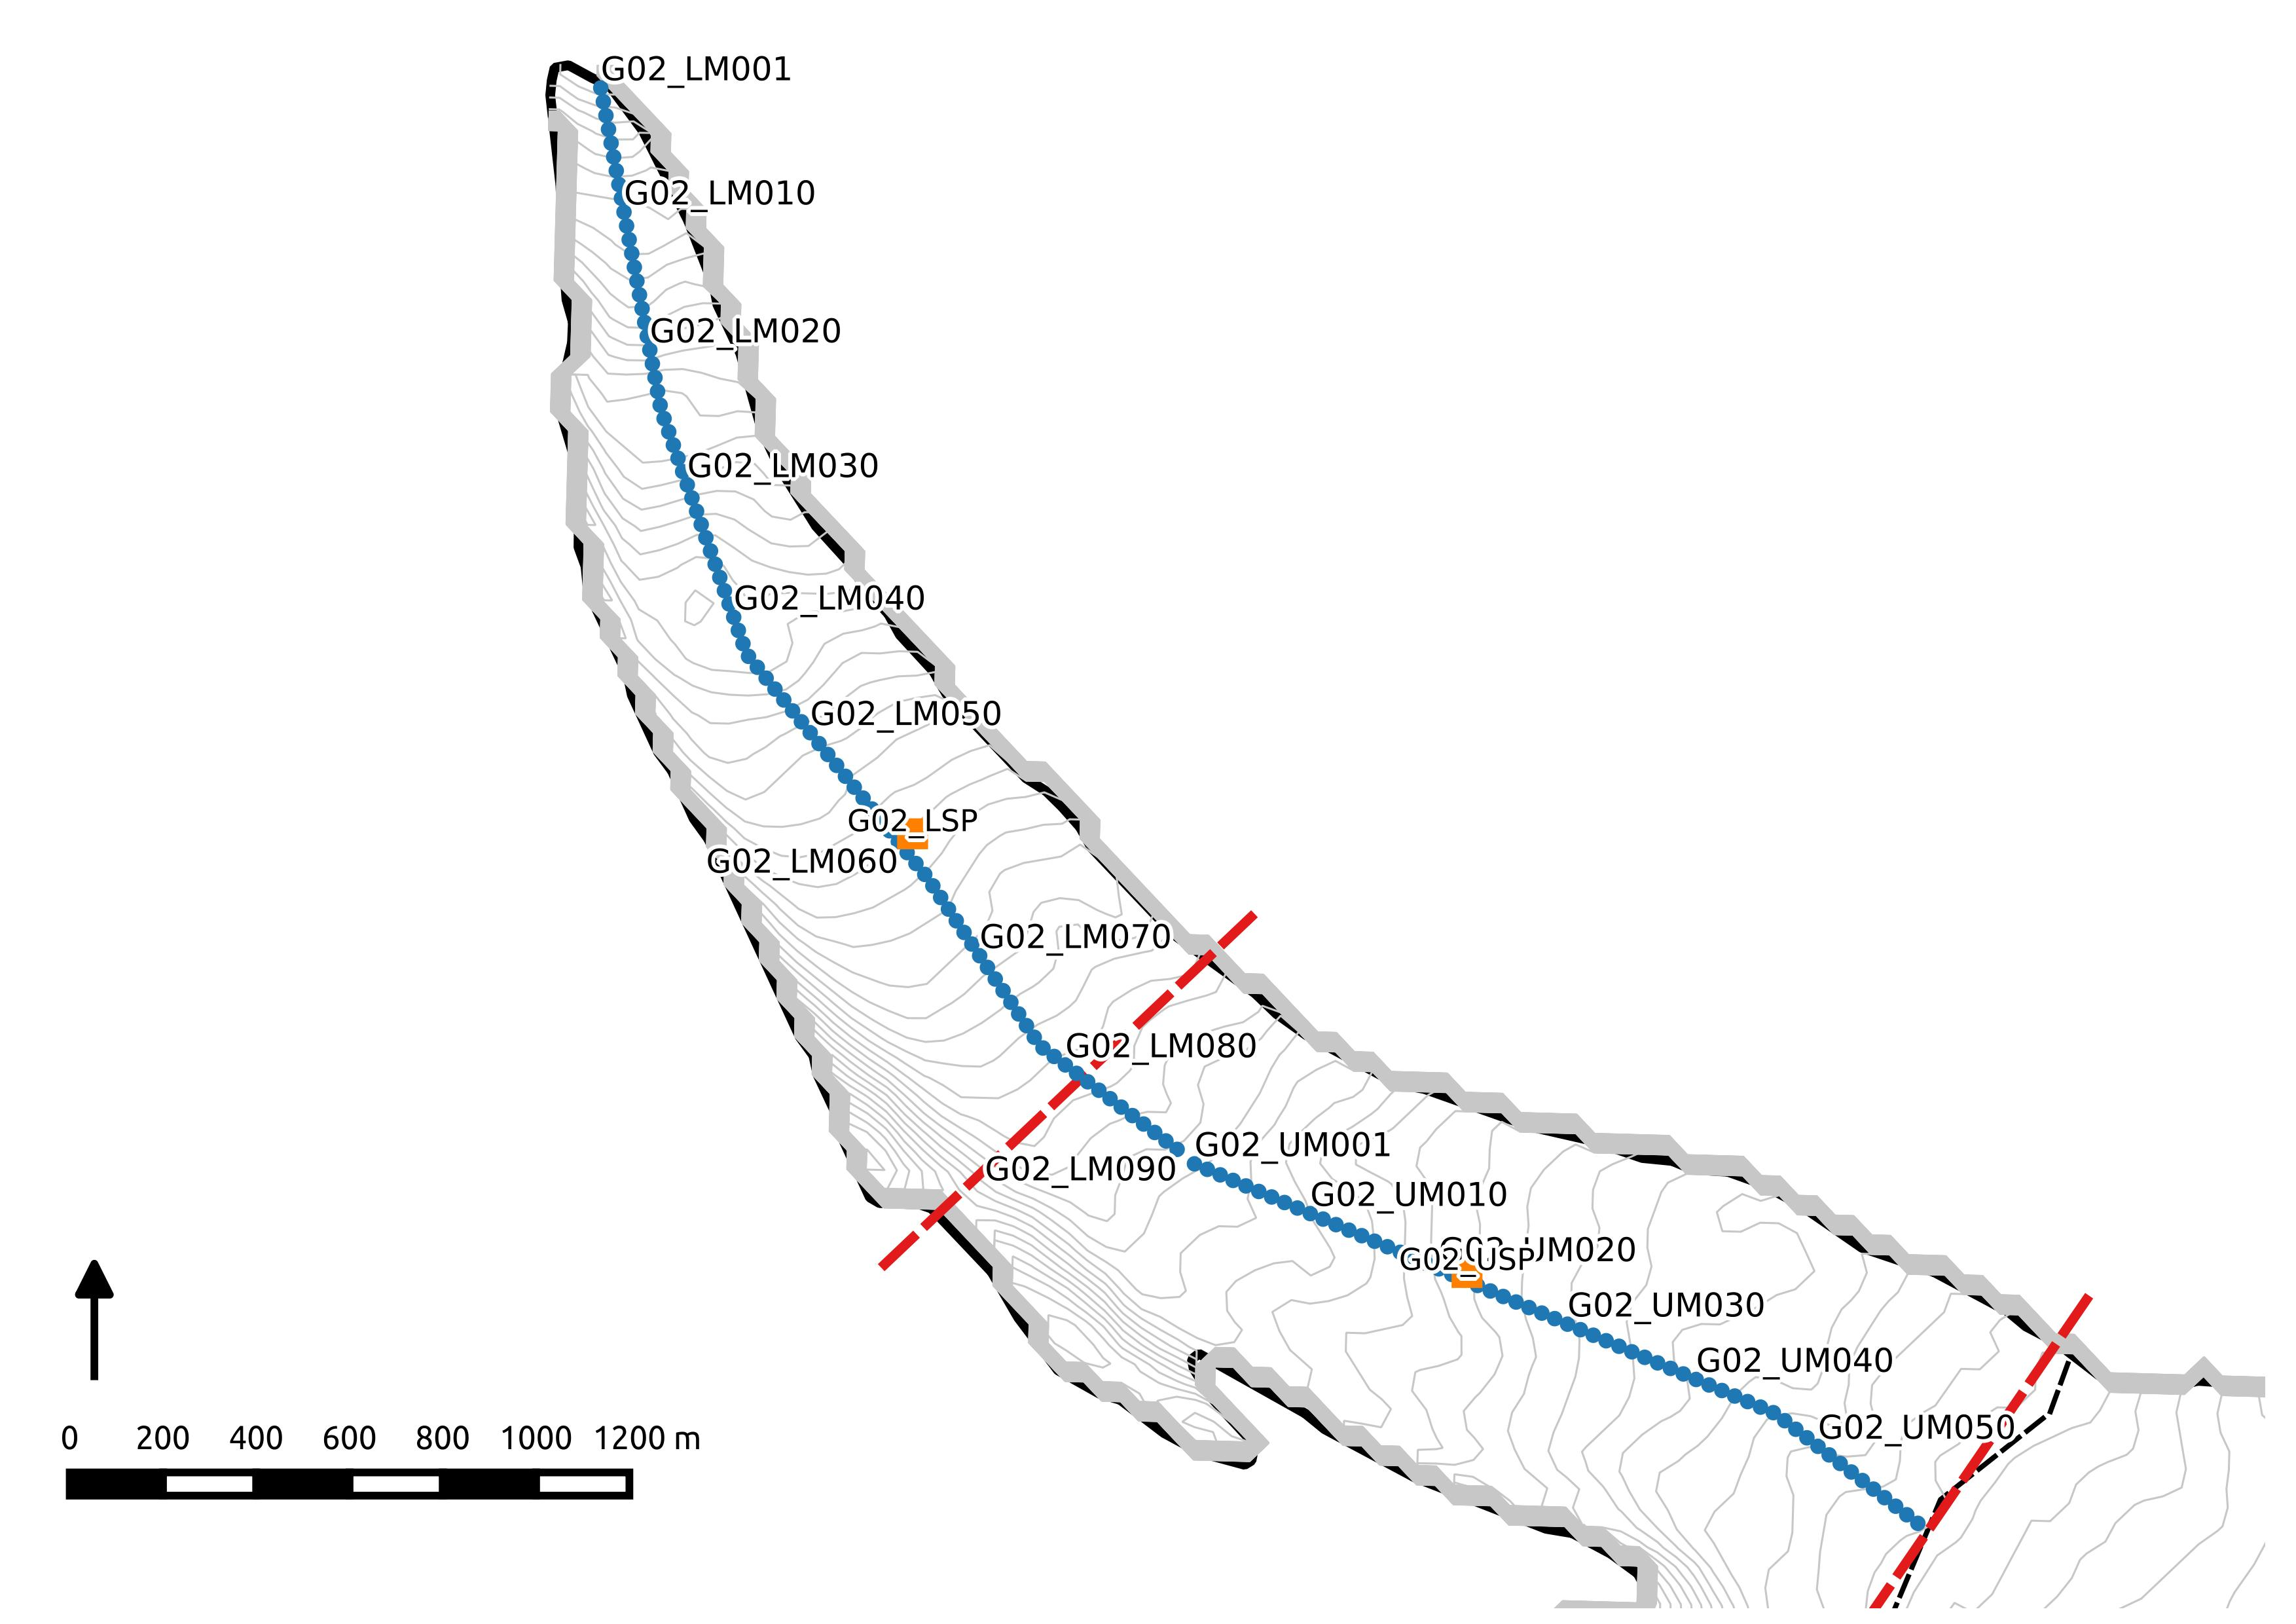
\includegraphics[height = 0.45\textheight]{G02_M.jpeg}}\\
\fbox{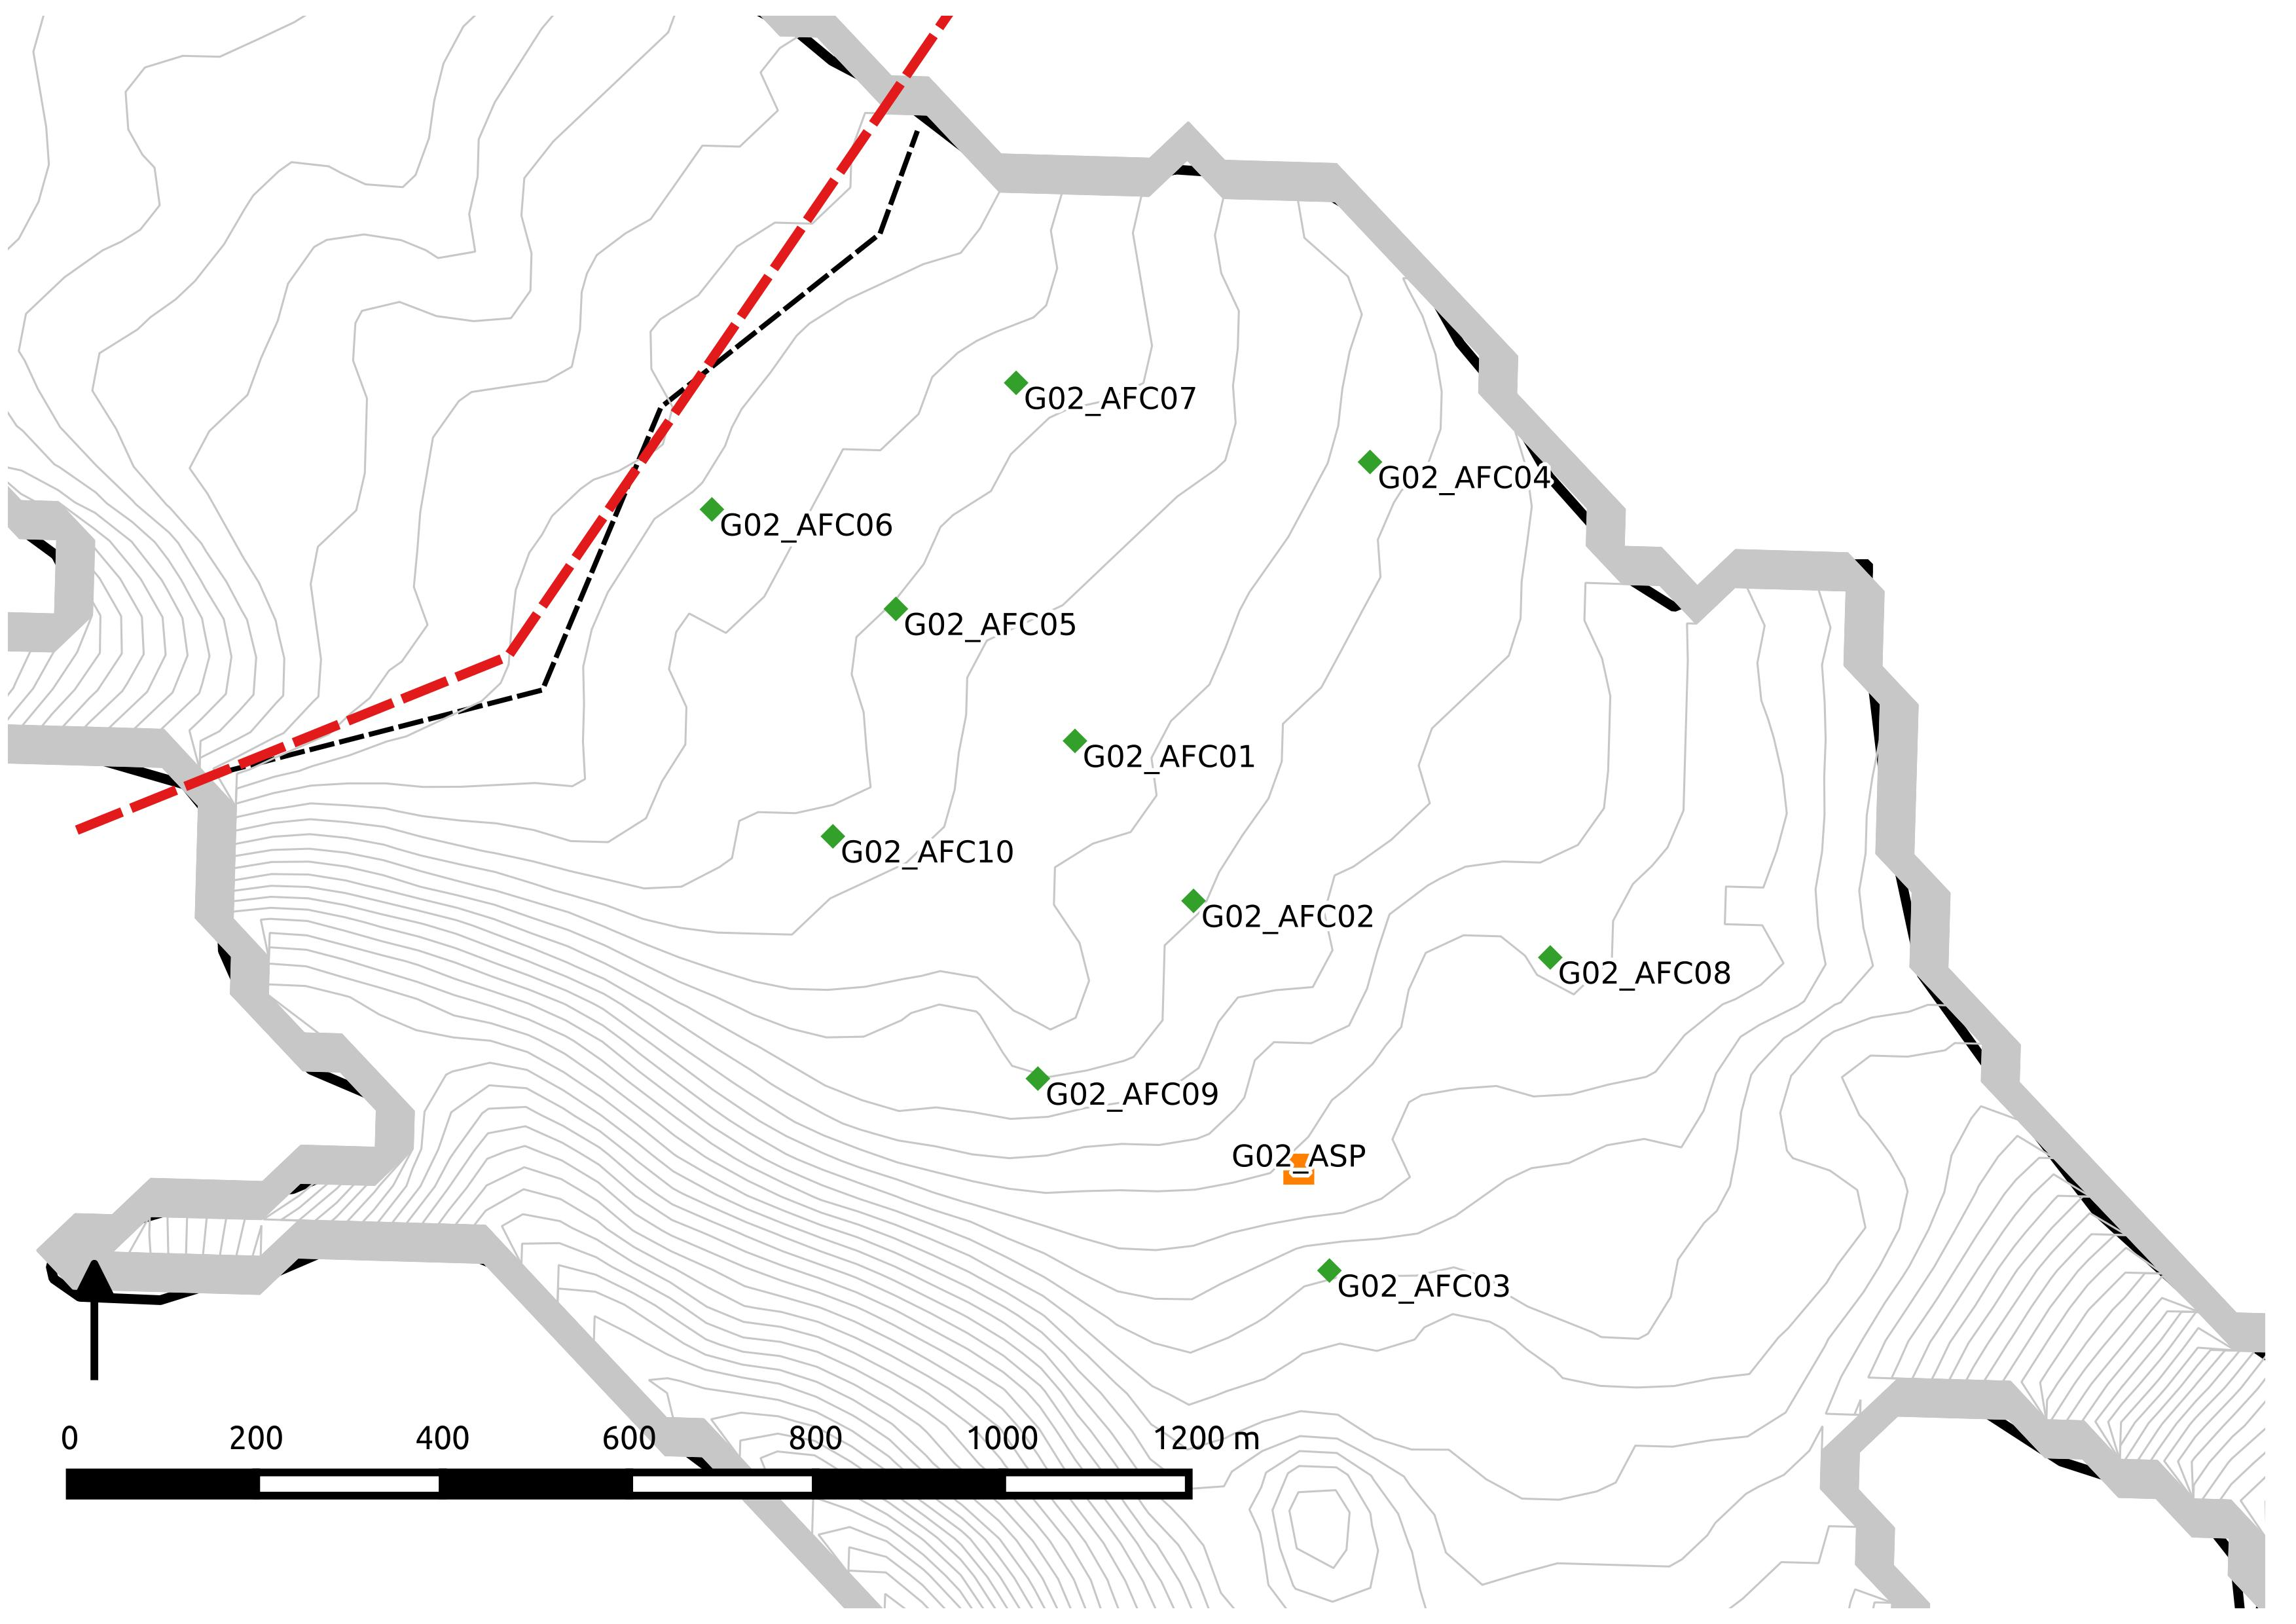
\includegraphics[height = 0.45\textheight]{G02_A.jpeg}}\\

\pagebreak
\noindent \large{\textbf{Glacier 13}}\\
\fbox{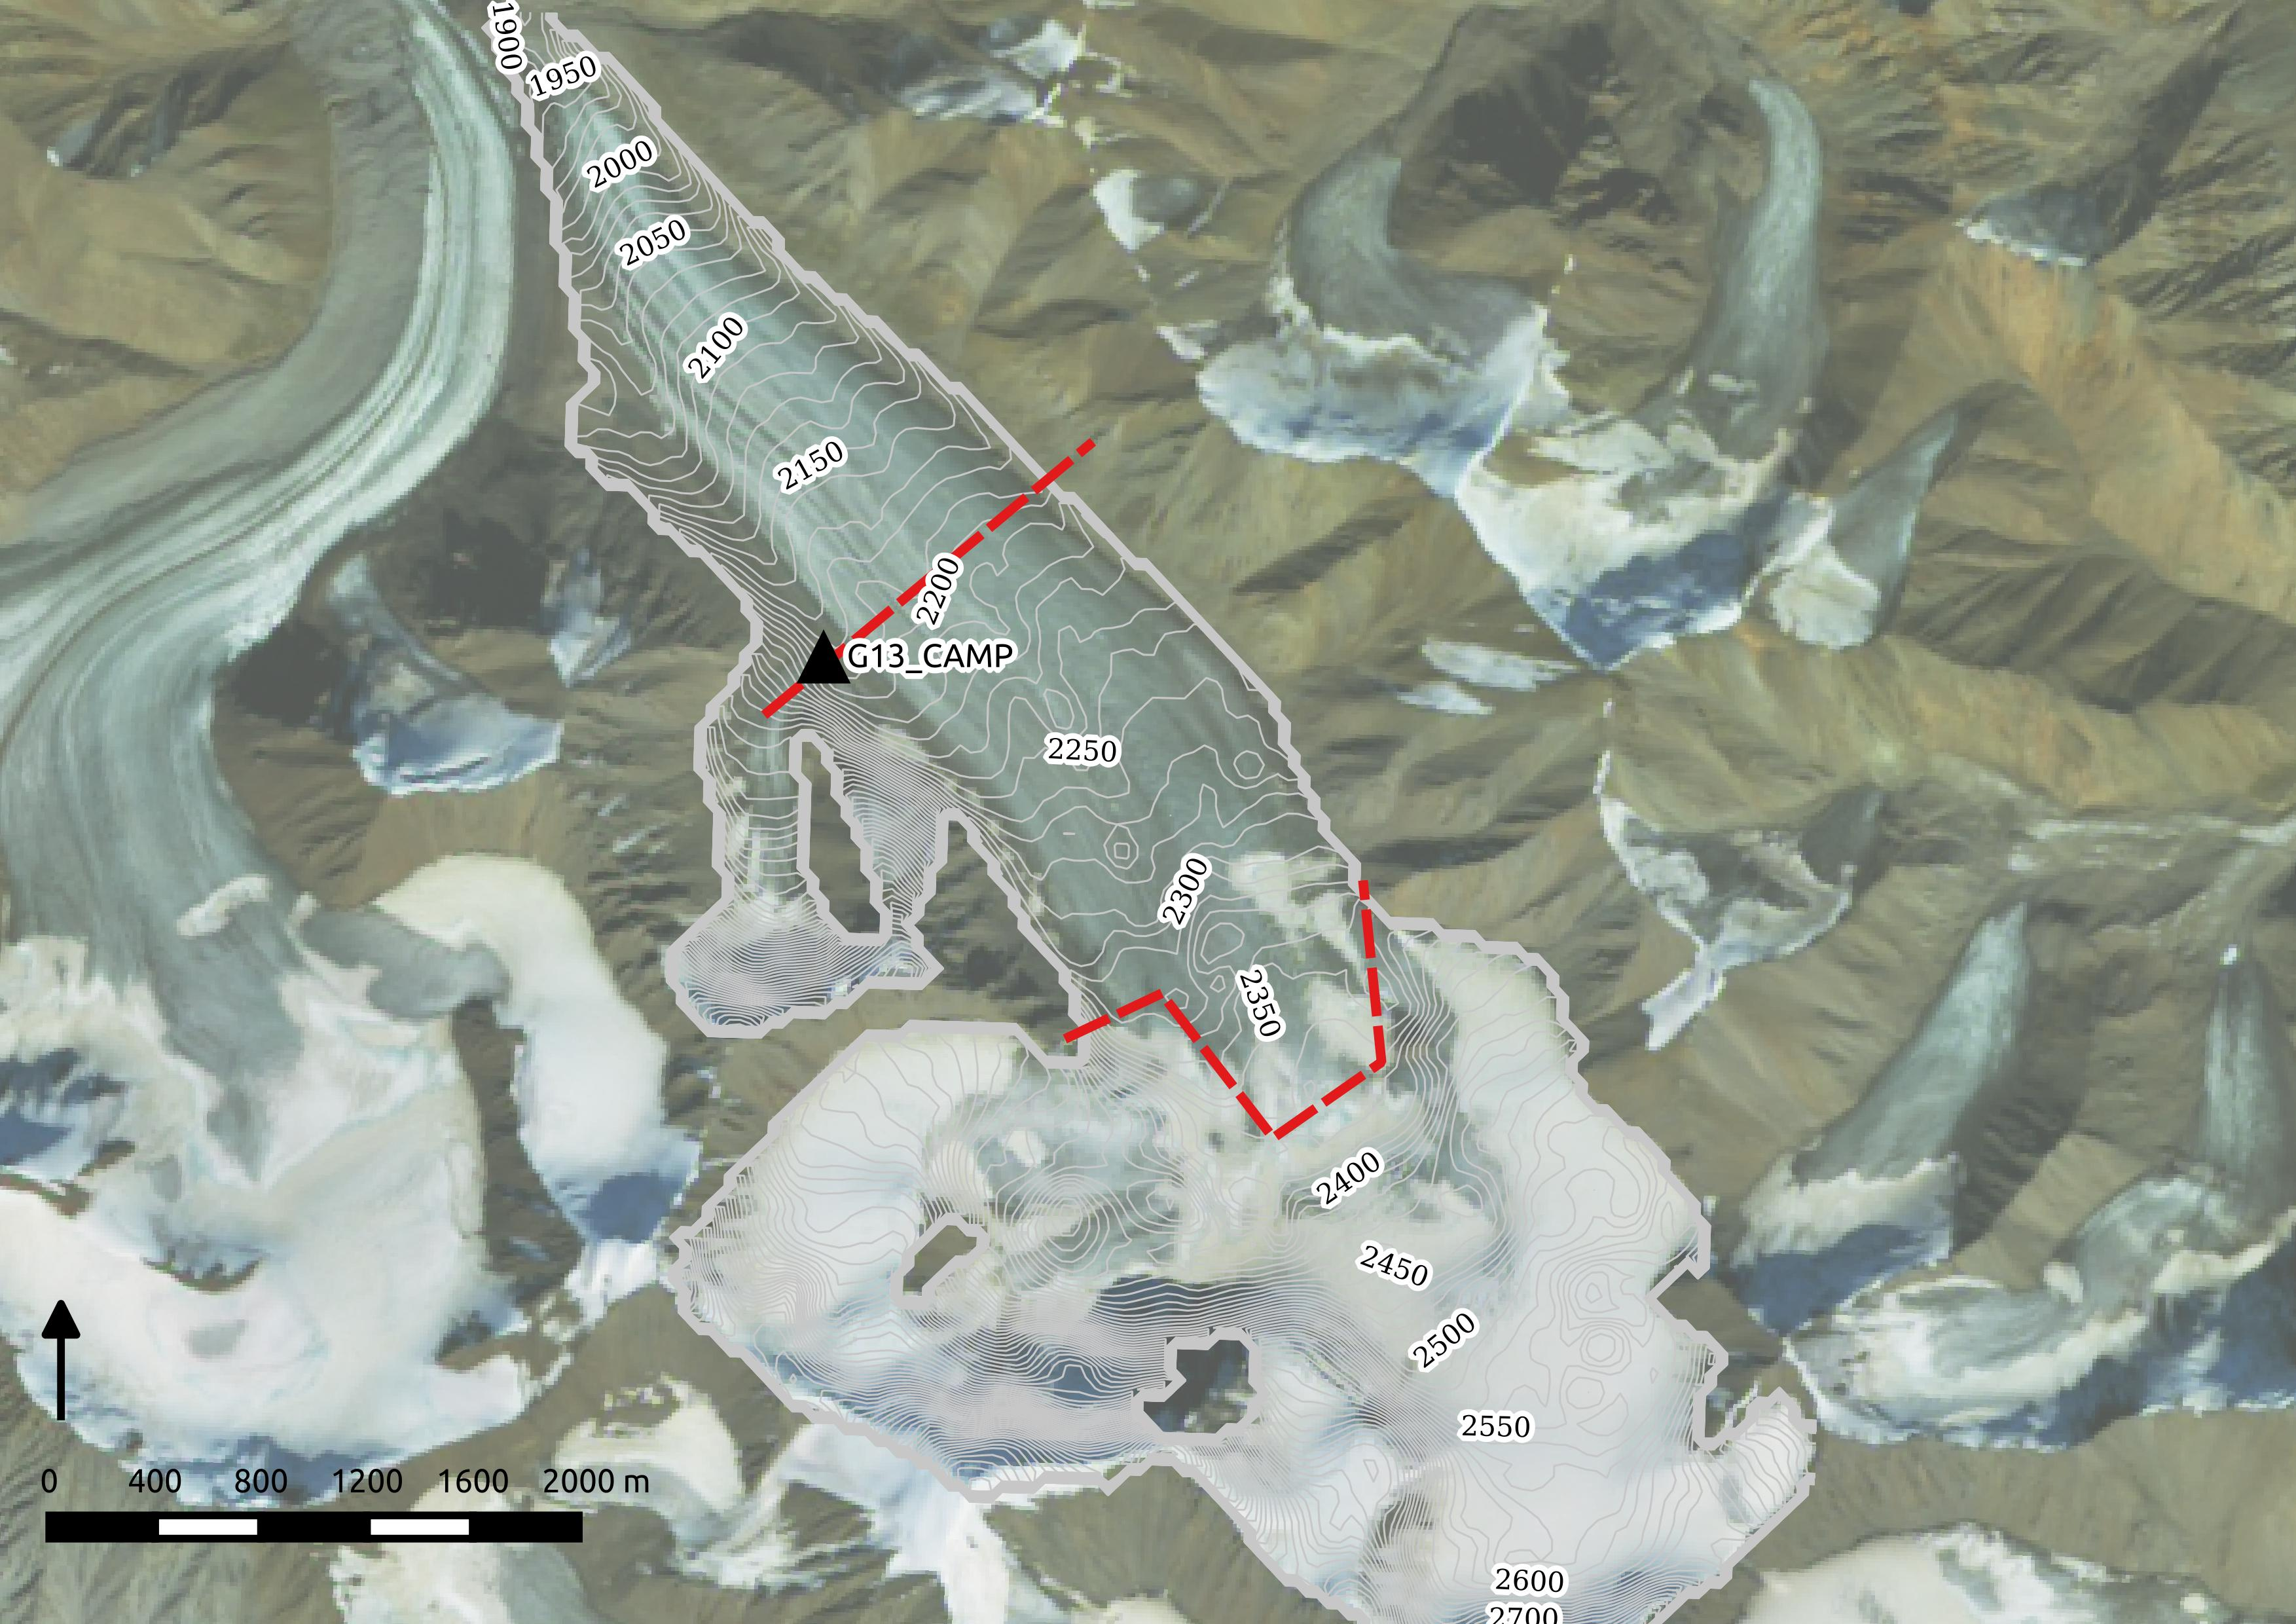
\includegraphics[height = 0.45\textheight]{G13_Topo.jpeg}}\\
\fbox{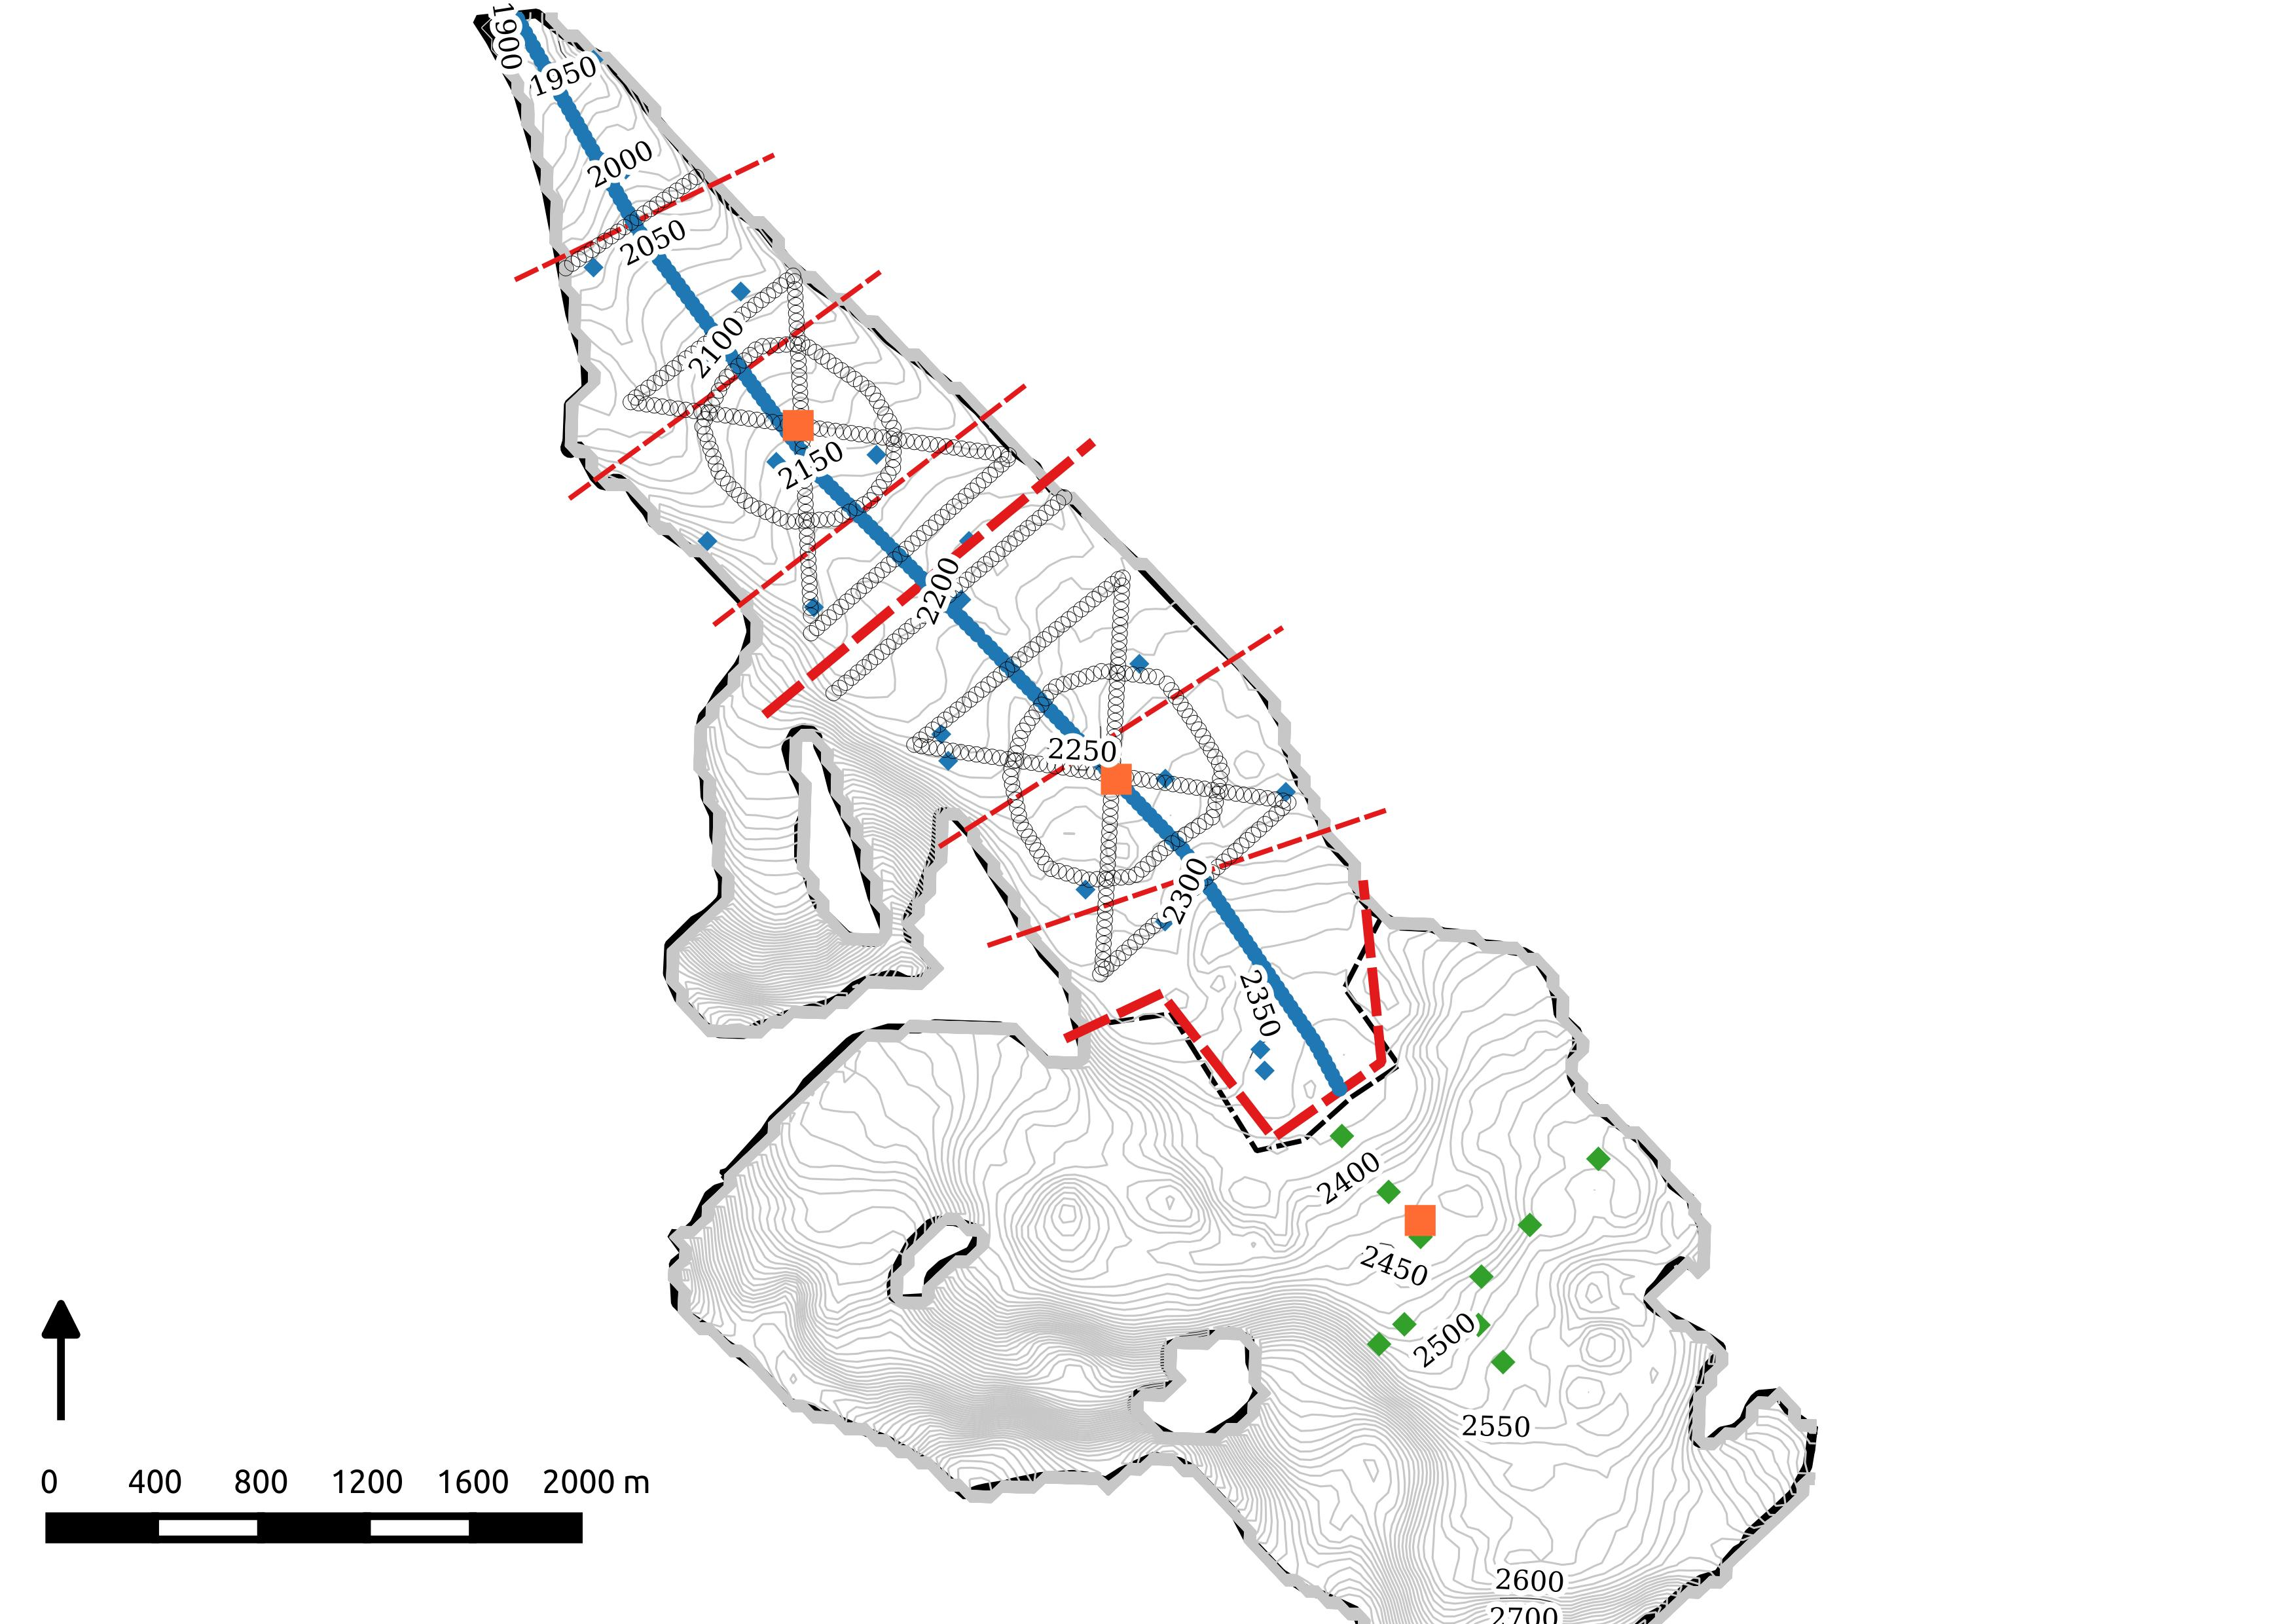
\includegraphics[height = 0.45\textheight]{G13_Overview.jpeg}}\\
\fbox{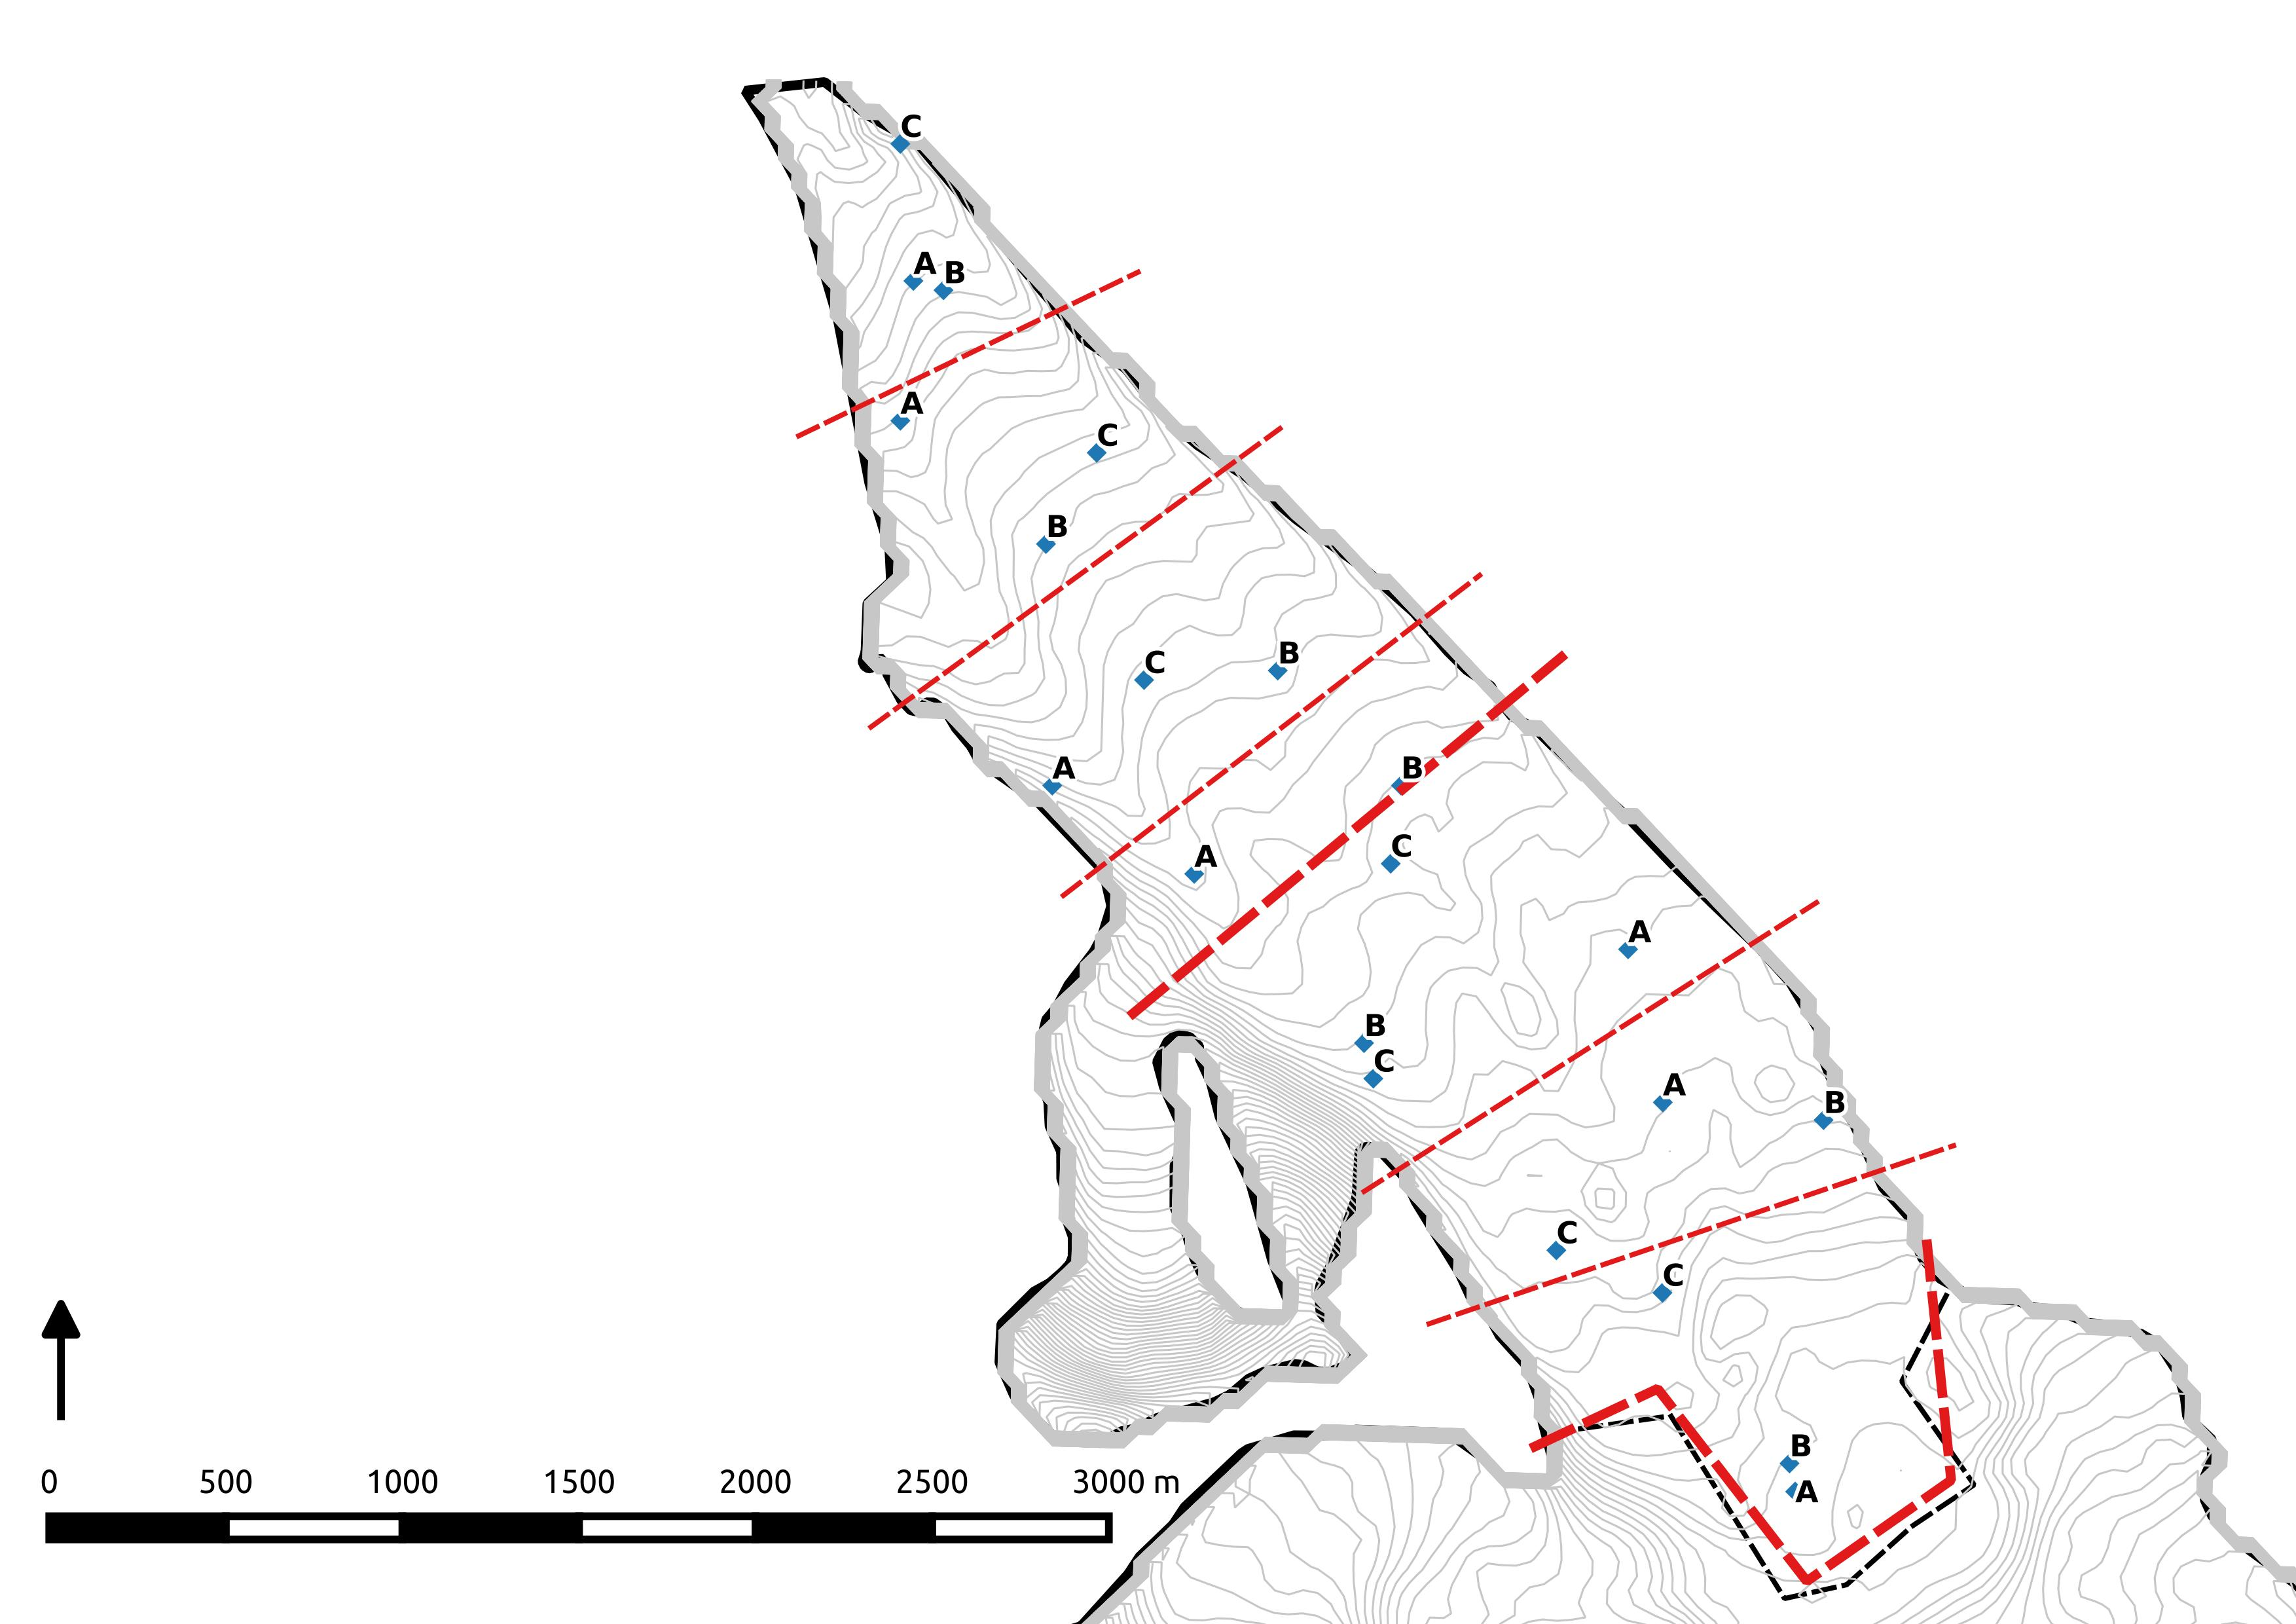
\includegraphics[height = 0.45\textheight]{G13_ZZ.jpeg}}\\
\fbox{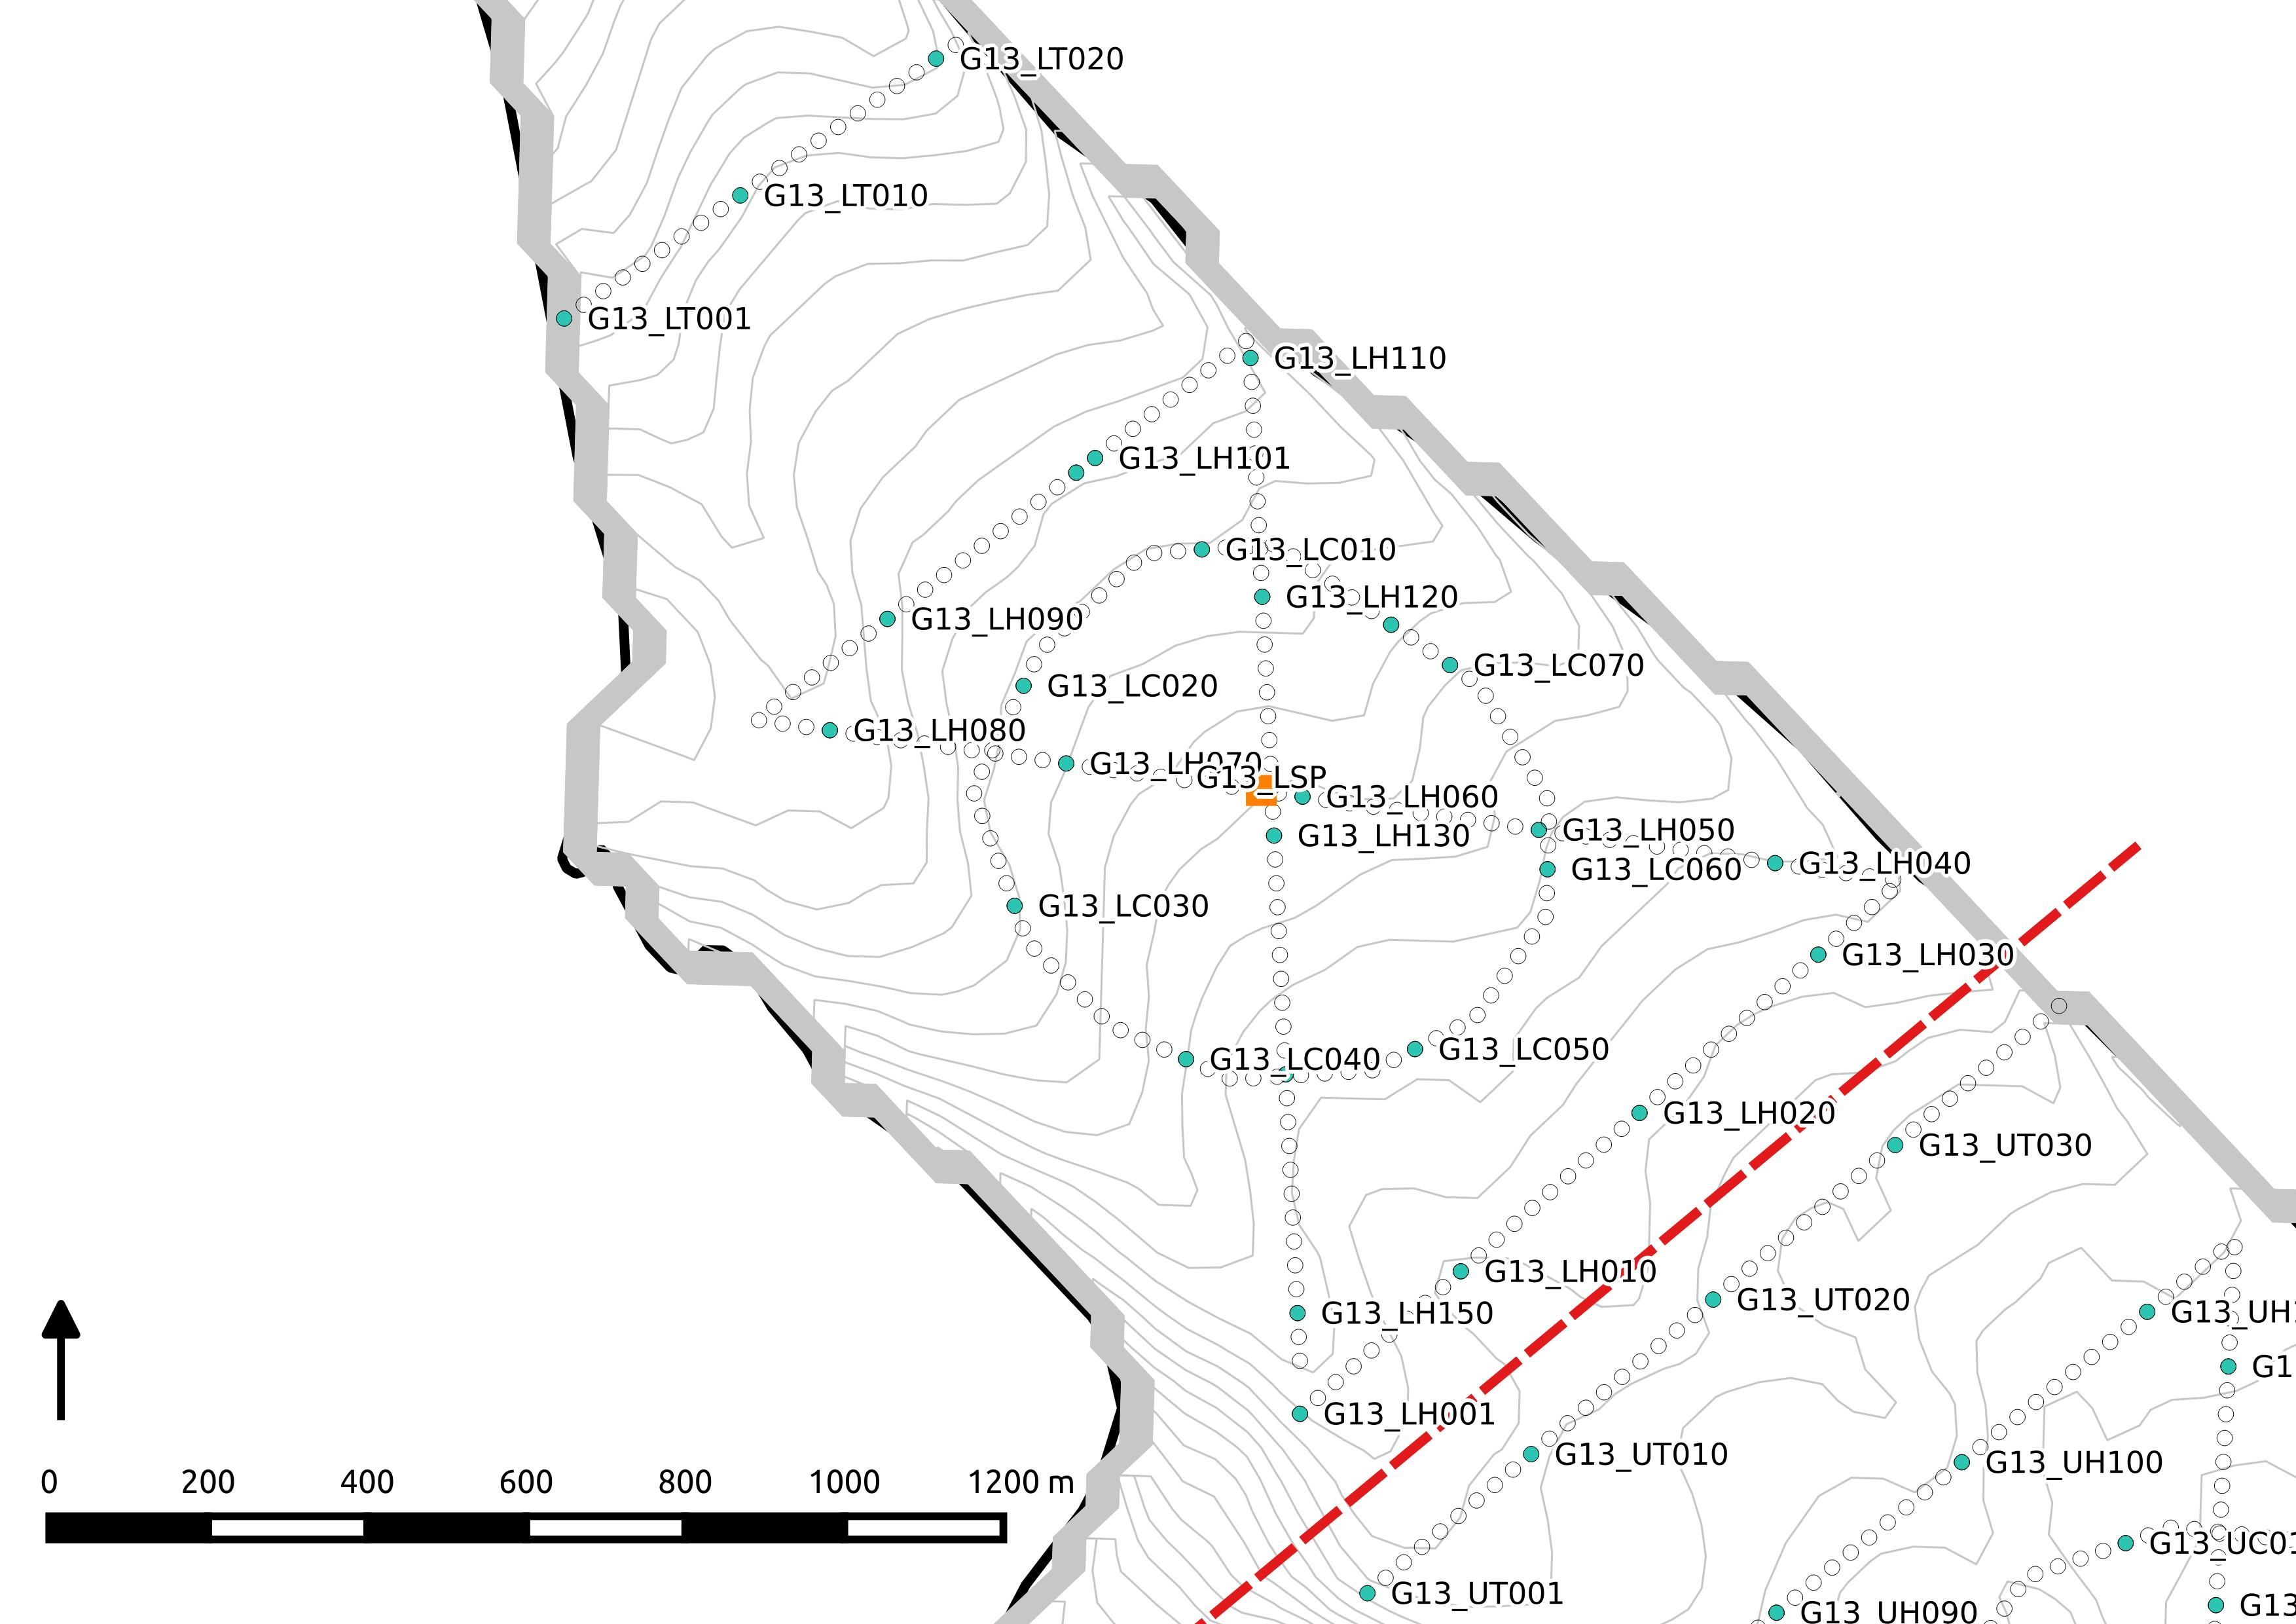
\includegraphics[height = 0.45\textheight]{G13_LH.jpeg}}\\
\fbox{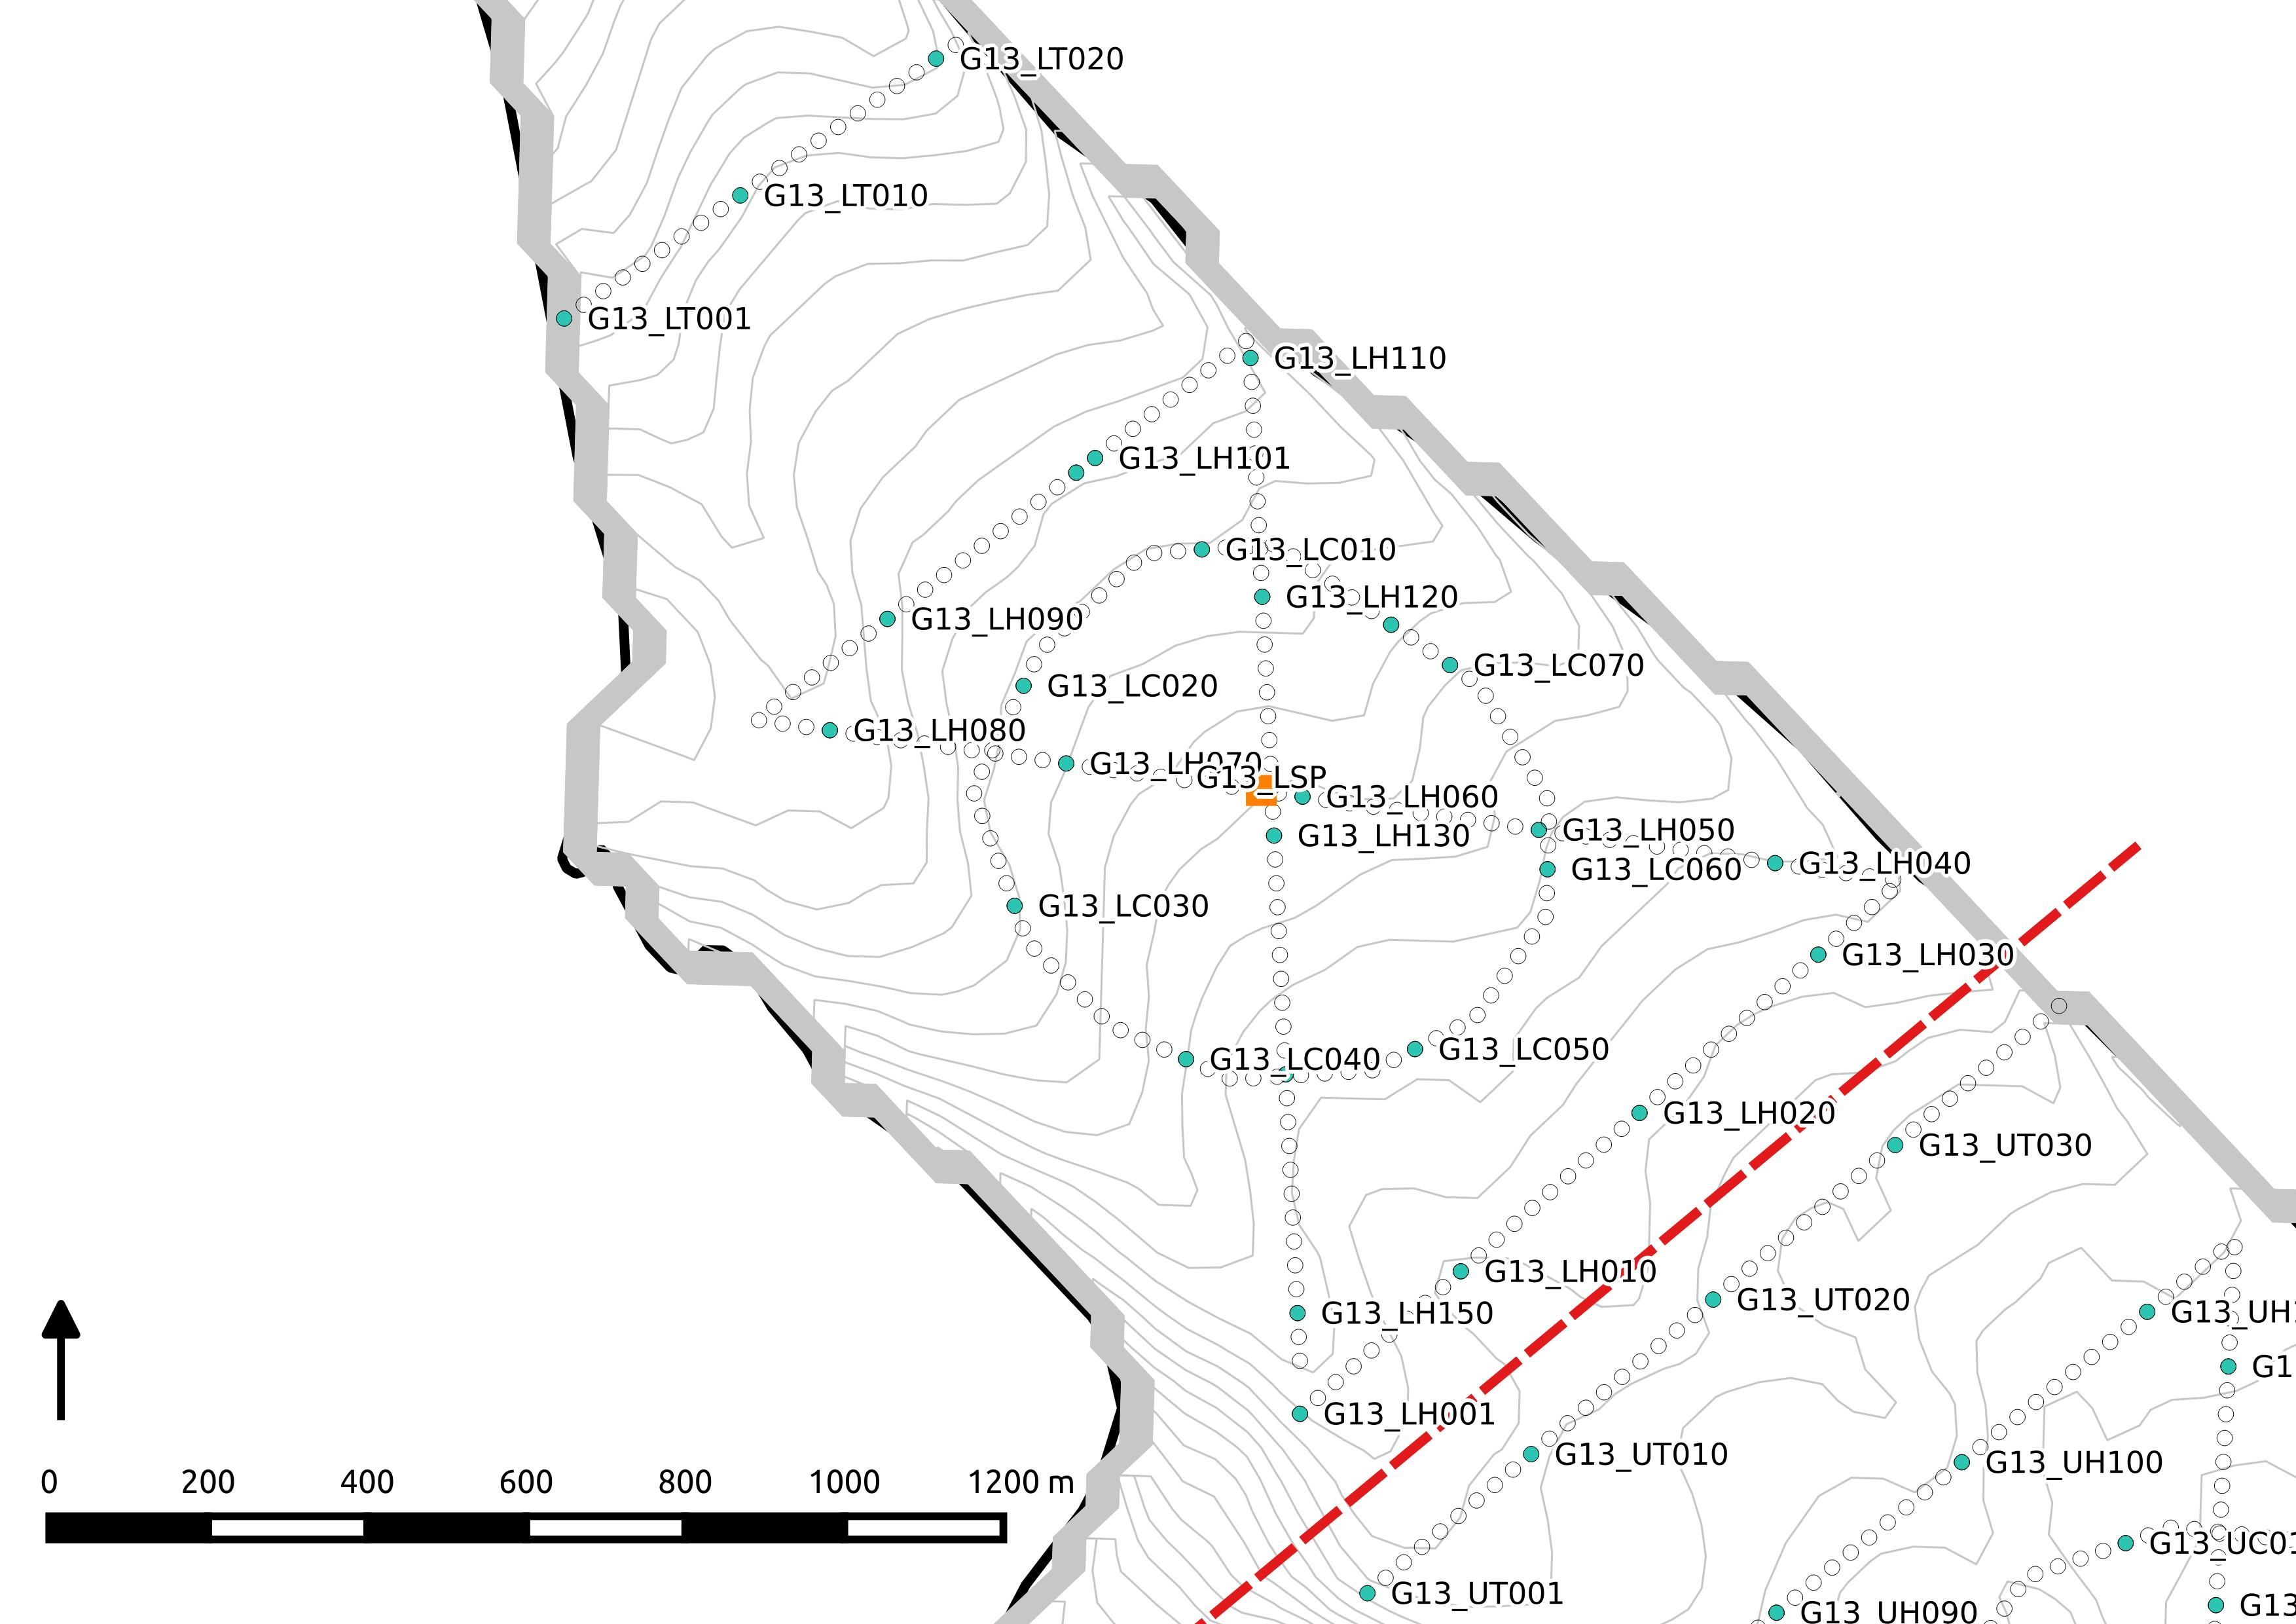
\includegraphics[height = 0.45\textheight]{G13_LH.jpeg}}\\
\fbox{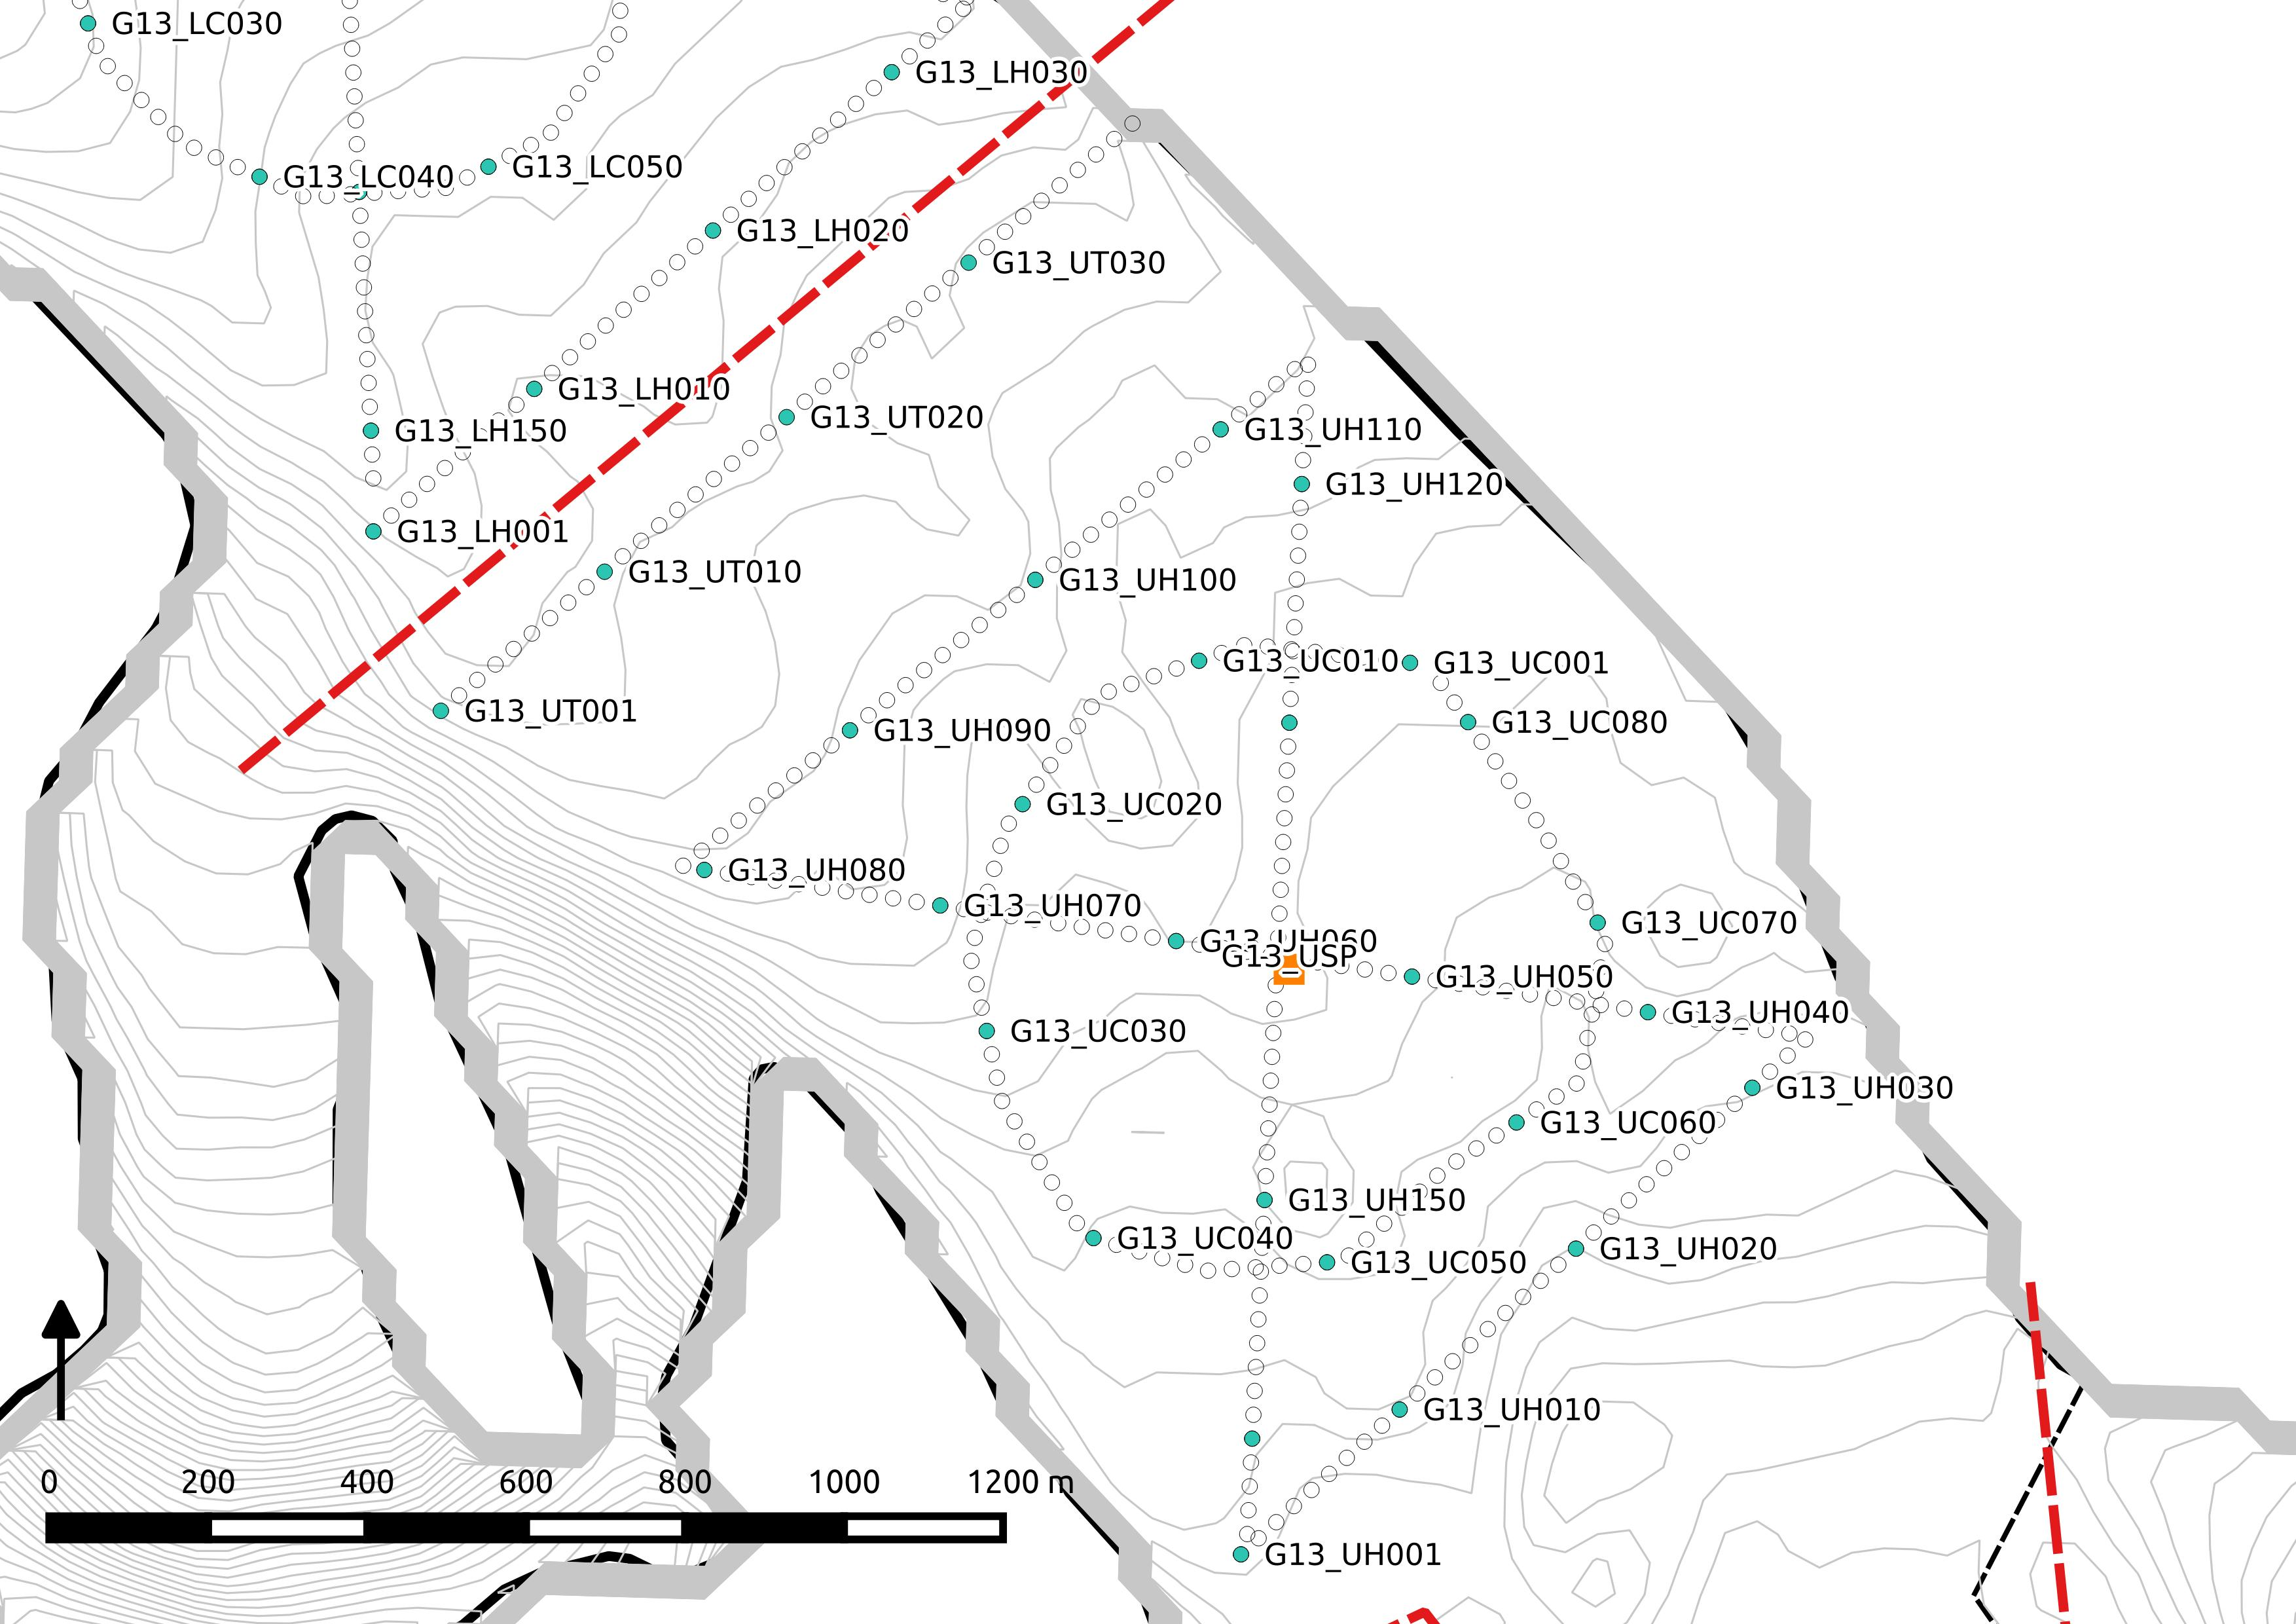
\includegraphics[height = 0.45\textheight]{G13_UH.jpeg}}\\
\fbox{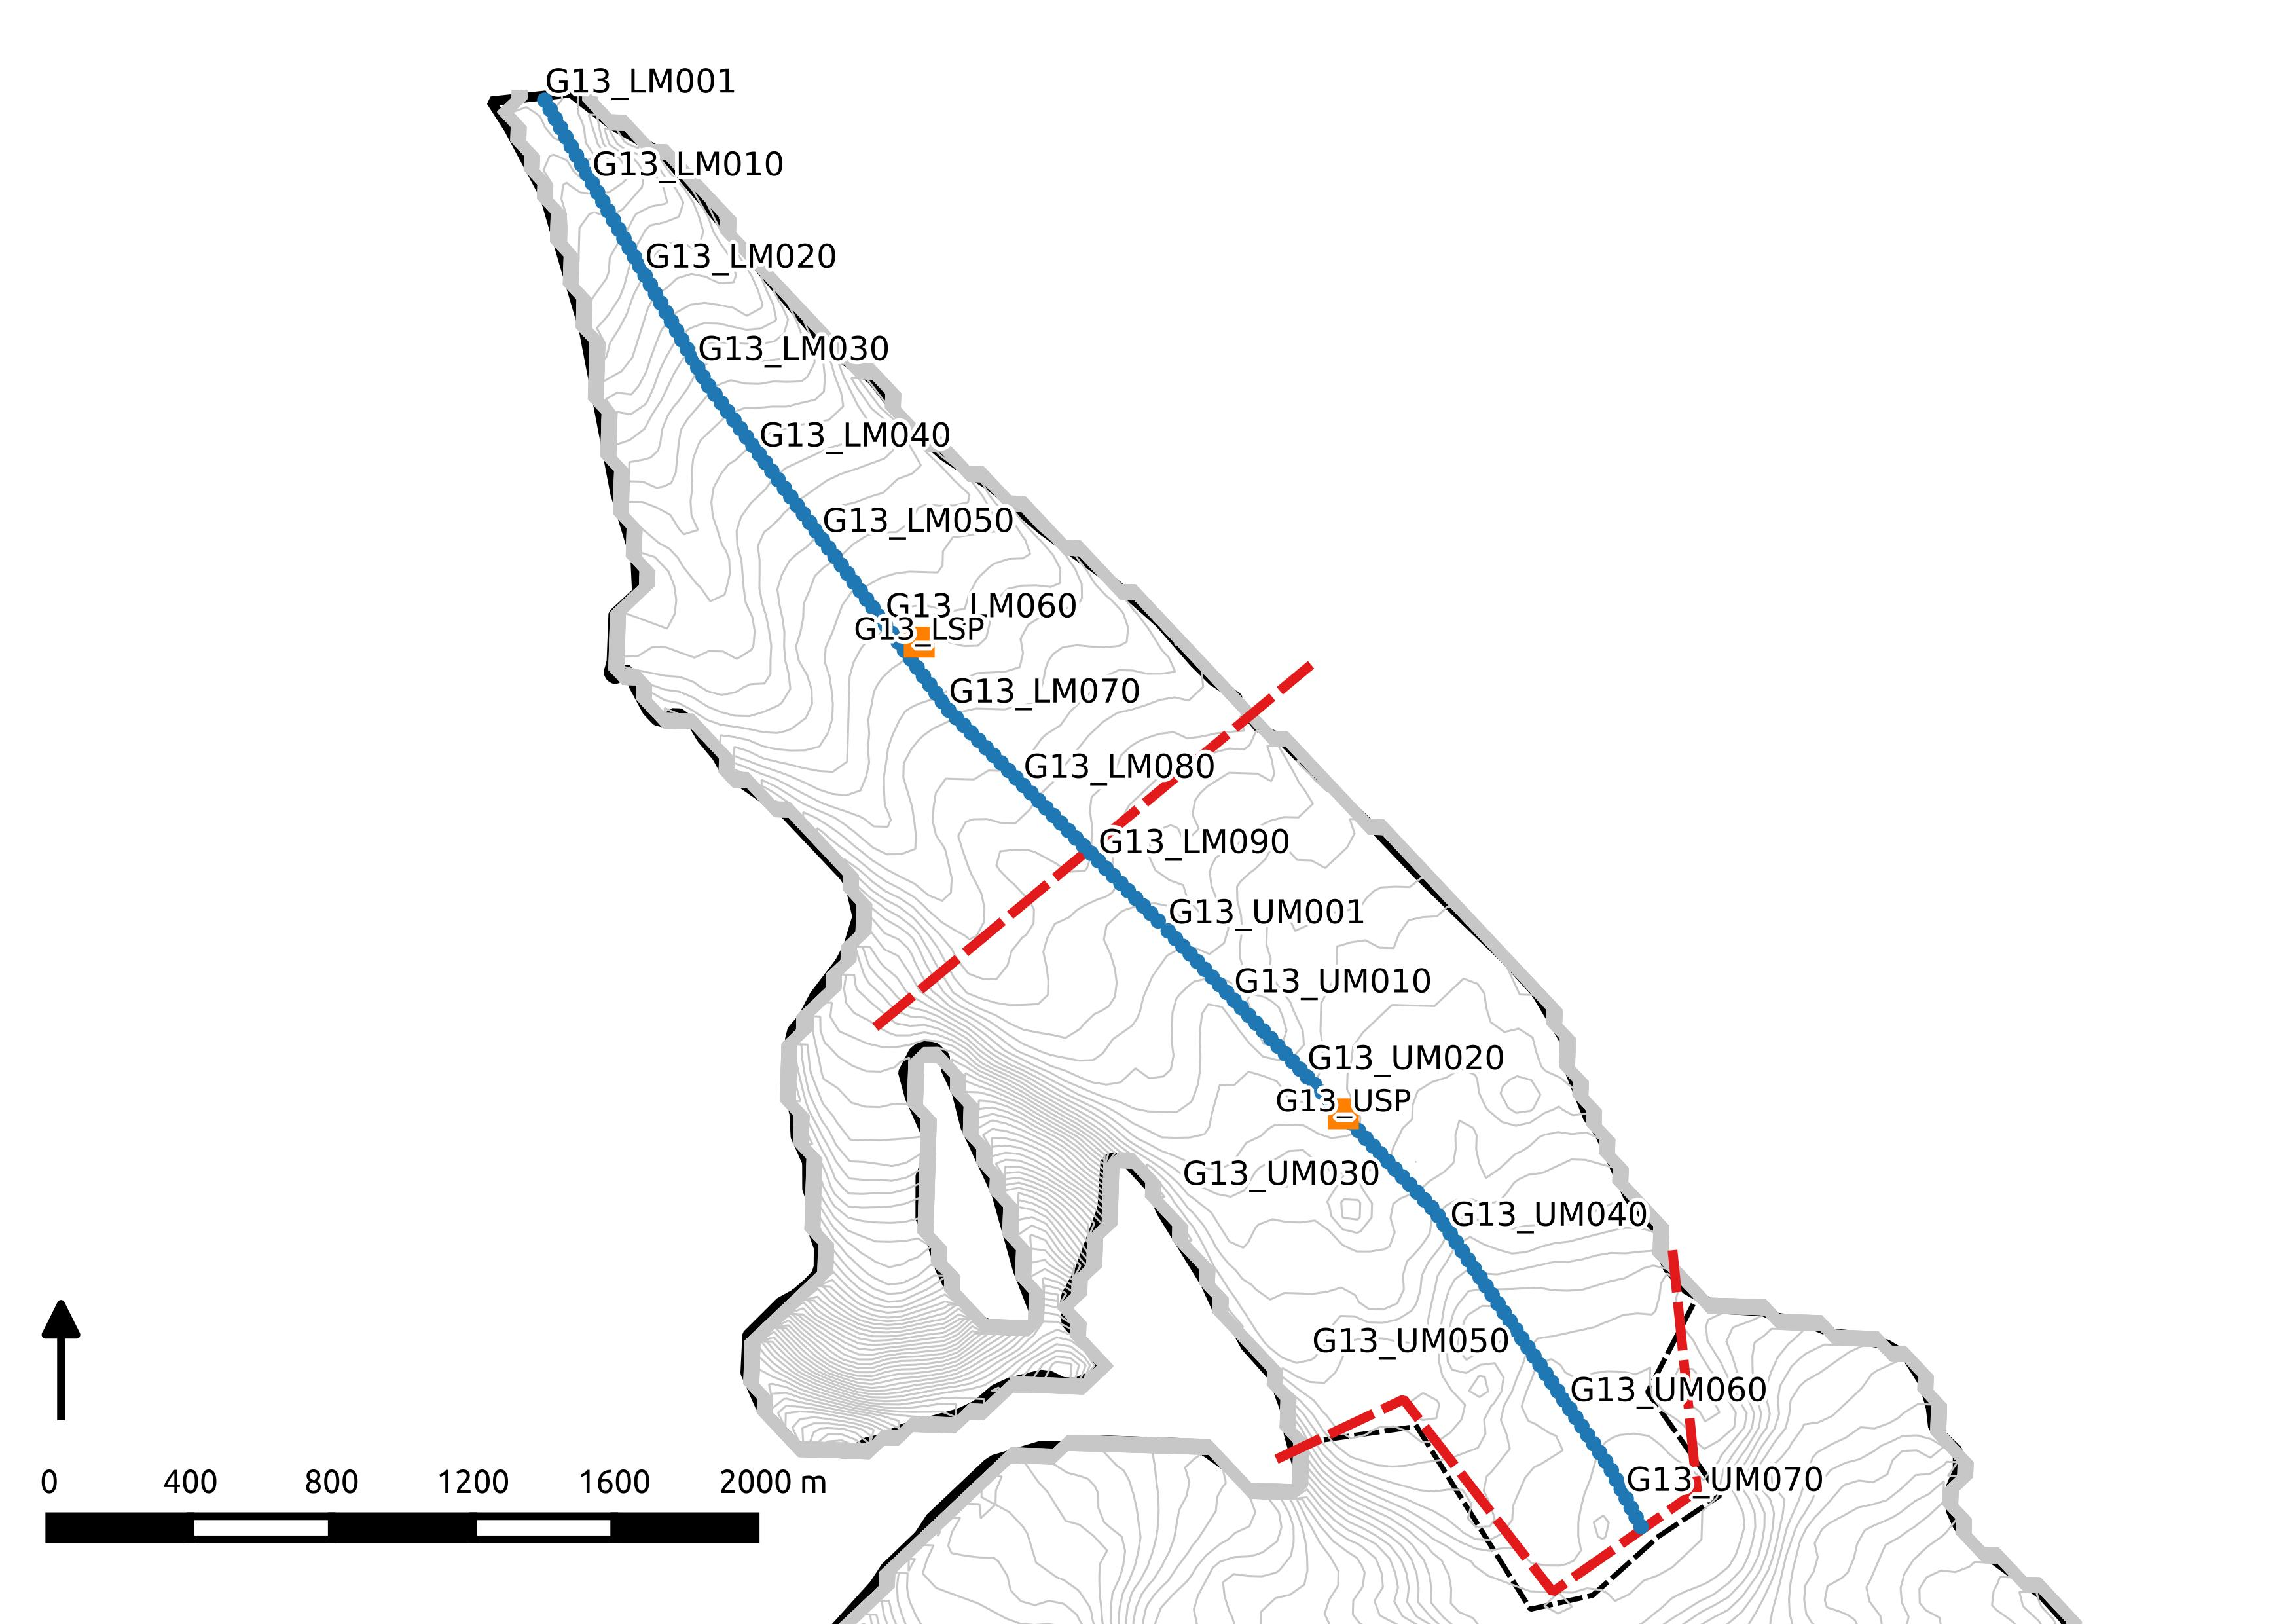
\includegraphics[height = 0.45\textheight]{G13_M.jpeg}}\\
\fbox{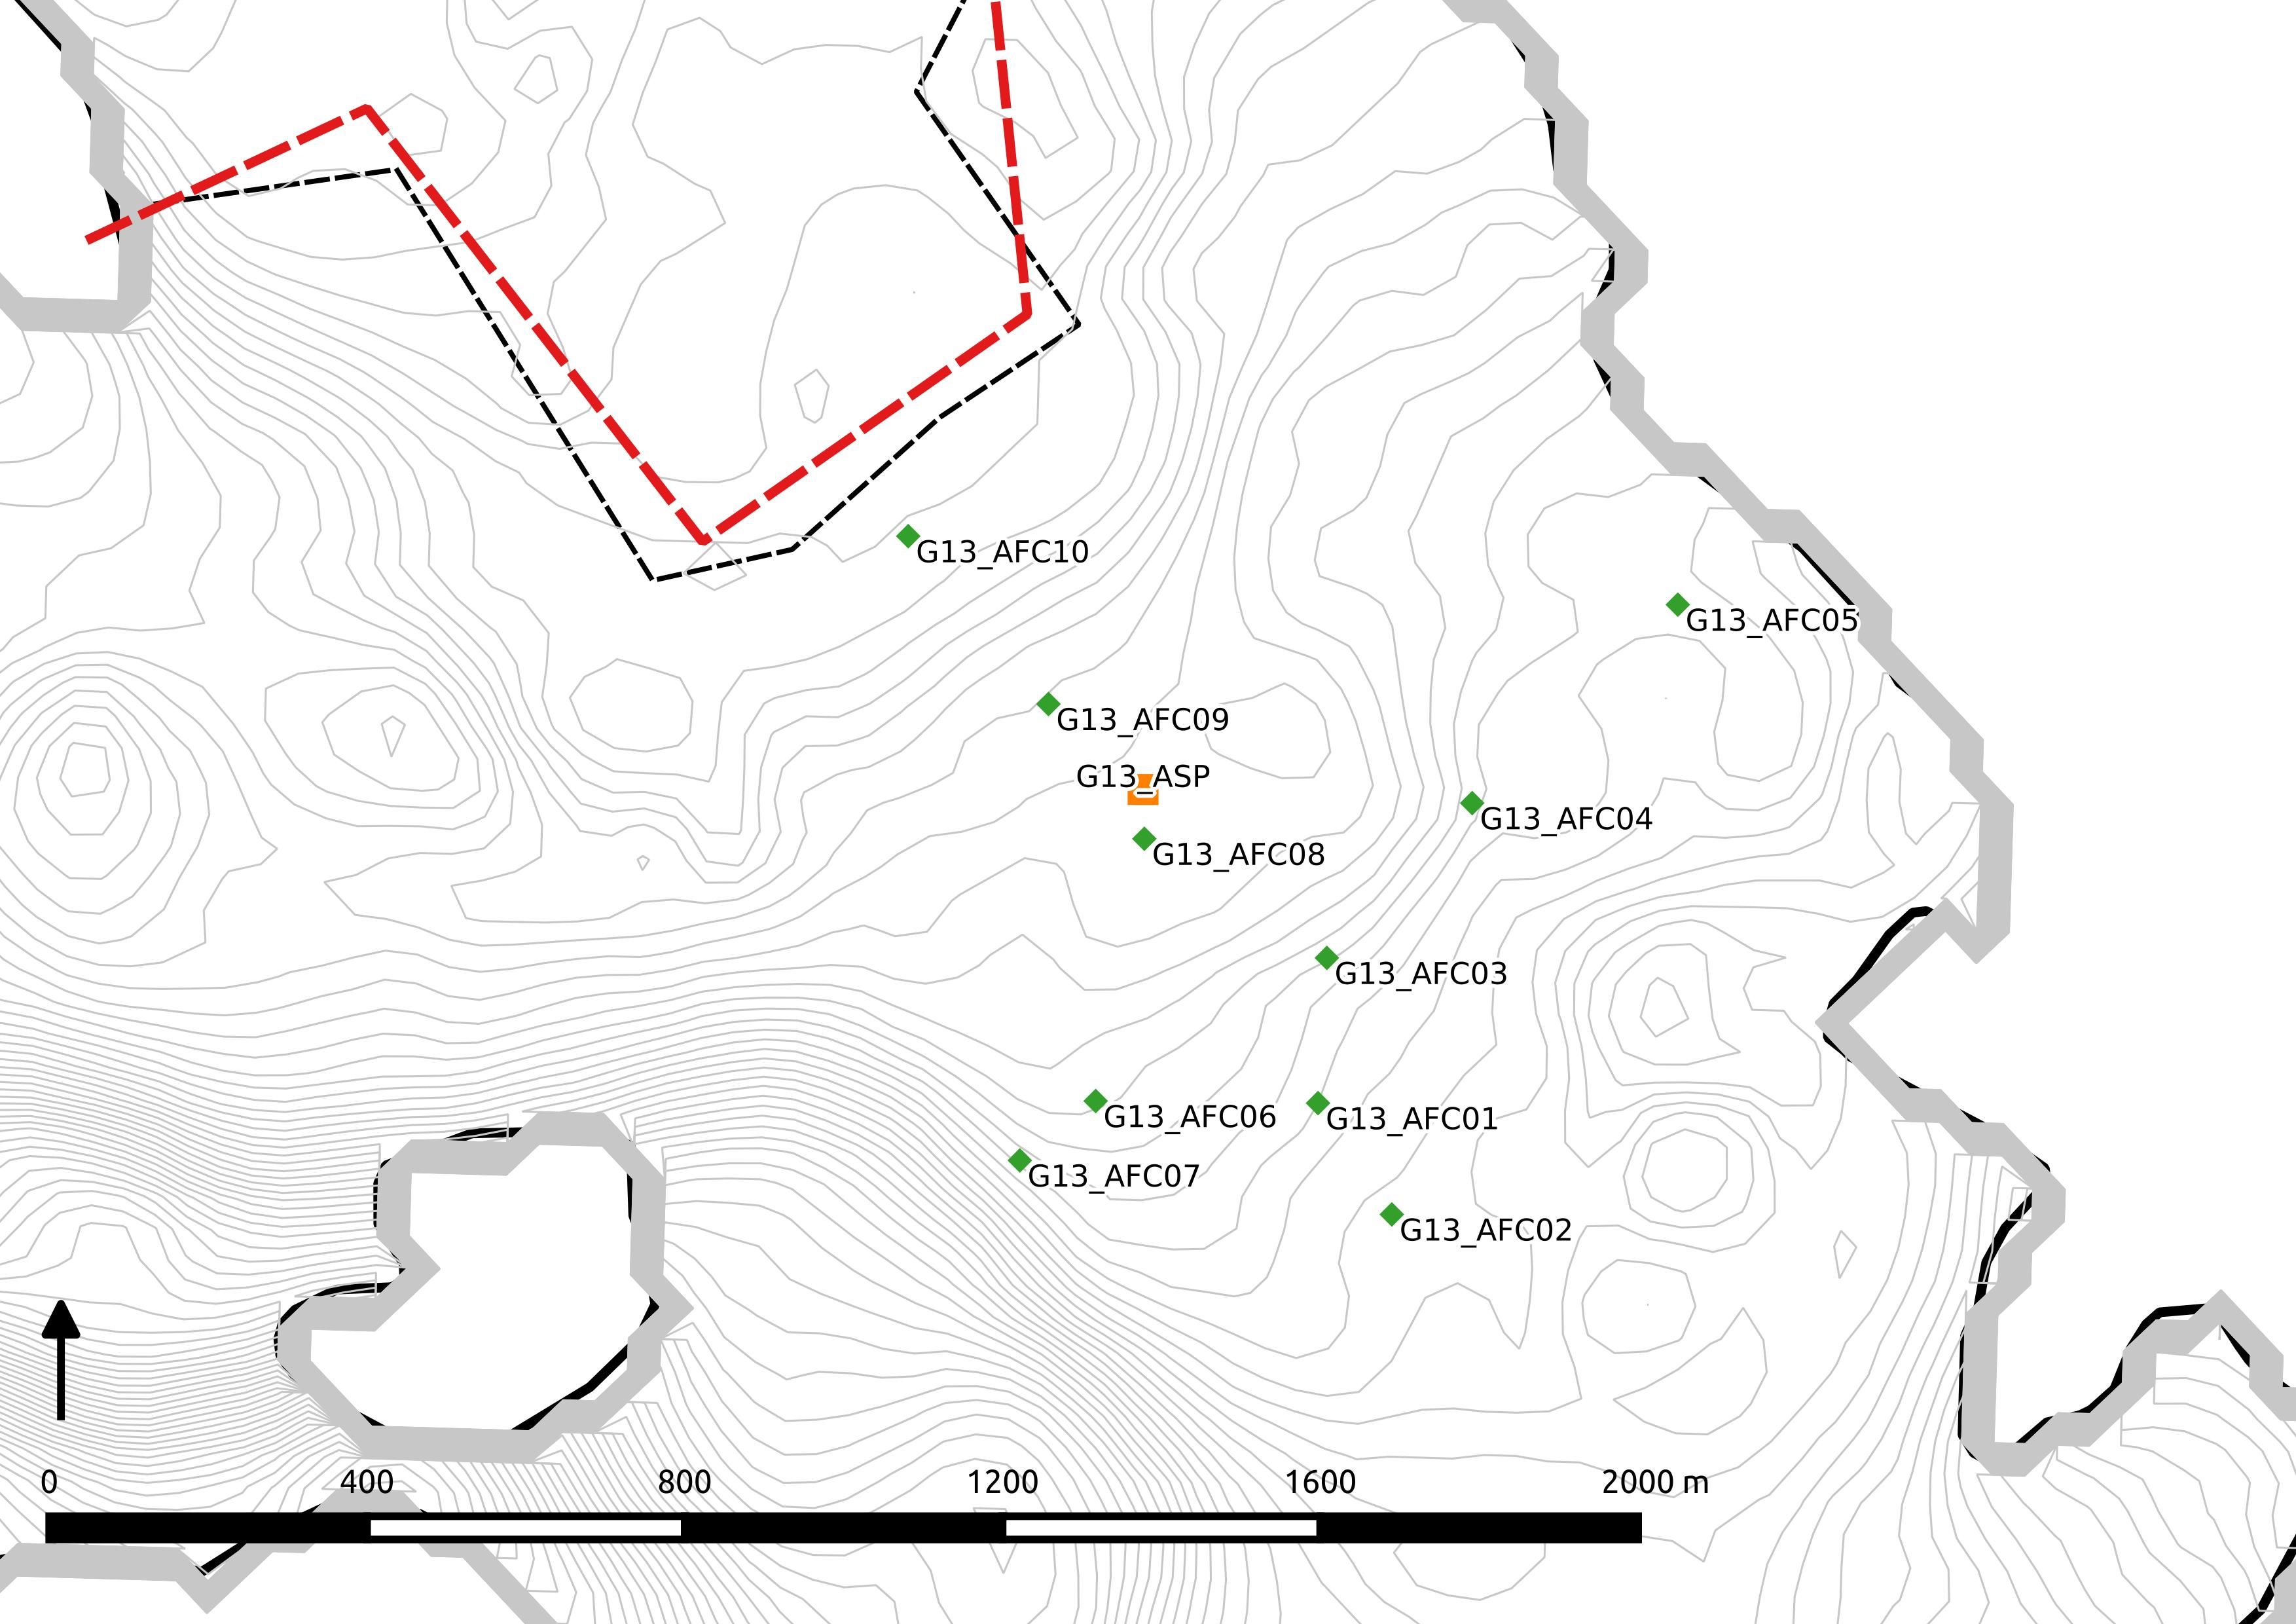
\includegraphics[height = 0.45\textheight]{G13_A.jpeg}}\\

\end{document}